\documentclass[10pt]{book}
\usepackage[utf8]{inputenc}
\usepackage{titlesec}
\usepackage{xspace}
\usepackage{microtype}
\usepackage{amssymb,amsmath,amsthm}
\newtheorem{theorem}{Theorem}
\newtheorem{lemma}{Lemma}
\usepackage{url}
\usepackage{graphicx}
\usepackage{caption}
\usepackage{subcaption}
\usepackage{enumitem}
\usepackage{hyperref}
% bold math
\usepackage{bm}
\usepackage{booktabs}
\usepackage{adjustbox}
\usepackage{array}
\usepackage{verbatim}
\usepackage{listings}
\usepackage{multicol}


% stuff like \ding for symbols
\usepackage{pifont}

\usepackage[
  natbib=true,
  style=alphabetic,
  backref=true,
  doi=false,
  isbn=false,
  maxbibnames=99,
]{biblatex}
\addbibresource{ref.bib}

\usepackage{epsfig}
\usepackage{textpos}
\usepackage{ifthen}
\usepackage{makeidx}
\usepackage{float}
\usepackage{calc}
\usepackage{vmargin}
\usepackage{letterspace}
\usepackage[pass]{geometry}

\usepackage{eurosym}
\usepackage{bytefield}
\usepackage[binary-units,detect-weight=true,detect-family=true]{siunitx}
\usepackage[usenames,dvipsnames,svgnames,table]{xcolor}
\usepackage{qrcode}
\usepackage{cryptocode}
\usepackage{tikz}
\usetikzlibrary{shapes,arrows}
\usetikzlibrary{positioning}
\usetikzlibrary{calc}
\usepackage{mdframed}
% Typography
\usepackage[sc,osf]{mathpazo}
\linespread{1.05}
\usepackage[scaled]{helvet} % ss
\usepackage{courier} % tt
\normalfont
\usepackage[T1]{fontenc}

\usepackage{pdfpages}

\author{Florian Dold \and the GNU Taler Developers}
\title{The GNU Taler System}

\begin{document}

\newcommand{\astfootnote}[1]{
\let\oldthefootnote=\thefootnote%
\setcounter{footnote}{0}%
\renewcommand{\thefootnote}{\fnsymbol{footnote}}%
\footnote{#1}%
\let\thefootnote=\oldthefootnote%
}

\frontmatter
\chapter{Abstract}
%As our society becomes more and more digitalized, an electronic version of cash
%becomes inevitable.  The design of payment systems is not just a technological
%matter, but has far-reaching sociopolitical consequences.
\begin{samepage}
We describe the design and implementation of GNU Taler, an electronic payment
system based on an extension of Chaumian online e-cash with efficient change.
In addition to anonymity for customers, it provides the novel notion of
\emph{income transparency}, which guarantees that merchants can reliably
receive a payment from an untrusted payer only when their income from the
payment is visible to tax authorities.

Income transparency is achieved by the introduction of a \emph{refresh
protocol}, which gives anonymous change for a partially spent coin without
introducing a tax evasion loophole.  In addition to income transparency, the
refresh protocol can be used to implement Camenisch-style \emph{atomic swaps}, and to
preserve anonymity in the presence of protocol \emph{aborts} and crash faults with
data loss by participants.

Furthermore, we show the provable security of our income-transparent anonymous
e-cash, which, in addition to the usual \emph{anonymity} and
\emph{unforgeability} properties of e-cash, also formally models
\emph{conservation} of funds and income transparency.

Our implementation of GNU Taler is usable by non-expert users and integrates
with the modern Web architecture.  Our payment platform addresses a range of
practical issues, such as tipping customers, providing refunds, integrating
with banks and know-your-customer (KYC) checks, as well as Web platform
security and reliability requirements.  On a single machine, we achieve
transaction rates that rival those of global, commercial credit card
processors.  We increase the robustness of the exchange---the component that
keeps bank money in escrow in exchange for e-cash---by adding an auditor
component, which verifies the correct operation of the system and allows to
detect a compromise or misbehavior of the exchange early.

Just like bank accounts have reason to exist besides bank notes, e-cash only
serves as part of a whole payment system stack.  Distributed ledgers have
recently gained immense popularity as potential replacement for parts of the
traditional financial industry.  While cryptocurrencies based on proof-of-work
such as Bitcoin have yet to scale to be useful as a replacement for established
payment systems, other more efficient systems based on blockchains with more
classical consensus algorithms might still have promising applications in the
financial industry.

We design, implement and analyze the performance of \emph{Byzantine Set Union
Consensus} (BSC), a Byzantine consensus protocol that agrees on a (super-)set
of elements at once, instead of sequentially agreeing on the individual
elements of a set.  While BSC is interesting in itself, it can also be used as
a building block for permissioned blockchains, where---just like in
Nakamoto-style consensus---whole blocks of transactions are agreed upon at once,
increasing the transaction rate.
\end{samepage}

\chapter*{Acknowledgements}

The book is based on Florian Dold's PhD thesis. We have removed the parts that
are not crucial for GNU Taler. Also, unlike the thesis, the GNU Taler project
continues to be updated, so this books is expected to be kept up-to-date with
the latest developments.  Nevertheless, Florian Dold's contribution to the
text remains fundamental.

We would like to thank Moritz Bartl for helping with the funding for Florian's
thesis and GNU Taler in general.  Bruno Haible provided generous support for
the GNU Taler team to visit meetings of the W3C's Web Payment Working Group.
We also thank Ashoka, the Tor project and the Donaukurier for their support.

This work benefits from the financial support of the Brittany Region (ARED
9174) and the Renewable Freedom Foundation (RFF).  

We thank the Bern University of Applied Sciences for continuing to host the
GNU Taler servers.

We thank to Cristina Onete and Jeff Burdges for their collaboration on the
provable security of GNU Taler.

We are grateful to the GNU project, in particular Richard Stallman, for their
support of this project.  We also thank all GNUnet developers and GNU Guix
developers, especially Hartmut Goebel, Nils Gillmann, Gabor Toth, Ludovic
Courtès and Andreas Enge.


\tableofcontents
\listoffigures
\mainmatter


\chapter{Introduction}\label{chapter:introduction}

New networking and cryptographic protocols can substantially improve
electronic online payment systems.  This book is about the design,
implementation and security analysis of GNU
Taler\footnote{\url{https://taler.net/}}, a privacy-friendly payment
system that is designed to be practical for usage as an online
(micro-)payment method, and at the same time socially and ethically
responsible.

Payment systems can generally be divided into two types: Register-based
and value-based~\cite{riksbank2017riksbank}.  A register-based system
associates value with identities (e.g., bank account balances with
customers), while a value-based system associates value with typically
anonymous, digital or physical tokens (such as cash or prepaid credit
cards).  In practice, these two types of systems are combined, as
different layers have different (and often conflicting) requirements:
the payment system used to pay for a cappuccino in a coffee shop is
most likely not suitable to buy real estate.  Value-based payment
systems typically provide more anonymity and convenience but also more
risk to consumers (as they are responsible to secure the values they
hold), while register-based systems shift risks to the payment service
provider who has to authenticate consumers and ensure the integrity of
the register.

This book explains GNU Taler, a design and implementation of a value-based
payment system, discussing in-depth how to create a practical,
privacy-preserving and secure (micro-)payment protocol that integrates nicely
with the modern web.  Our value-based payment protocol can in principle
operate on top of any existing register-based system.

GNU Taler is an official package of the GNU
project\footnote{\url{https://gnu.org/}}.  Our free software implementation is
freely available from the GNU mirrors.


\section{Design Goals for GNU Taler}

The design of payment systems shapes economies and societies
\cite{zandi2013impact,dalebrant2016monetary}.  Payment systems with high
transaction costs create an economic burden.  Predominantly cash-based
societies provide some degree of anonymity for their citizens, but can fail to
provide a sound foundation for taxation, facilitate corruption
\cite{singh2017does} and thus risk creating weak governments. On the other
hand, systems with too much surveillance eliminate personal freedom.

As the Internet has no standardized payment system, especially not one
that is capable of quickly, efficiently and securely settling small
transactions (so-called micropayments), the majority of content on the web is
financed by advertisements.  As a result, advertising (and by
implication, collecting data on users) has been a dominant business
model on the Internet.  This has not only resulted in a loss of
independence of publishers---who need to cater to the needs
of advertisers---but also in a situation where micro-targeted ads
are so wide-spread, that they have been suspected to have influenced
multiple major elections~\cite{persily2017election}.  Ads are also a
vector for malware \cite{provos2007ghost}.  Due to the prevalence of
ad blockers, ads are also not guaranteed to be a sustainable business
model.

In the world of online payments, credit cards and a sprawling number
of smaller, proprietary payment processors are currently dominant, and
market shares vary widely between different
countries~\cite{adyen2016global,paypers2016ecommerce}.  The resulting
fragmentation again increases social costs: online shops can either
choose to invest in implementing many proprietary protocols, or only
implement the most popular ones, thereby reinforcing the dominance of
a handful of proprietary payment systems.

Considering these and other social implications of payment systems, we
started the development of GNU Taler with a set of high-level design
goals that fit our social agenda.  They are ranked by the importance
we give to them, and when a trade-off must be made, the one that
supports the more highly ranked goal is preferred:

% what about micropayments -> part of 'efficient'
\begin{enumerate}
  \item \textbf{GNU Taler must be implemented as free software.}

    Free refers to ``free as in free speech'', as opposed to ``free as in free beer''.
    More specifically, the four essential freedoms of free software
    \cite{stallman2002essays} must be respected, namely users must have the
    freedom to (1) run the software, (2) study and modify it, (3) redistribute
    copies, and (4) distribute copies of the modified version.

    For merchants this prevents vendor lock-in, as another payment provider can
    take over, should the current one provide inadequate quality of service.
    As the software of
    the payment provider itself is free, smaller or disadvantaged countries or
    organizations can run the payment system without being controlled by a
    foreign company.  Customers benefit from this freedom, as the wallet
    software can be made to run on a variety of platforms, and user-hostile
    features such as tracking or telemetry could easily be removed from
    wallet software.

    This rules out the mandatory usage of specialized
    hardware such as smart cards or other hardware security modules, as the
    software they run cannot be modified by the user.  These components can,
    however, be voluntarily used by merchants, customers or payment processors
    to increase their operational security.

  \item \textbf{GNU Taler must protect the privacy of buyers.}\label{item:privacy}

    Privacy should be guaranteed via technical measures, as opposed to mere
    policies.  Especially with micropayments for online content, a
    disproportionate amount of rather private data about buyers would be revealed, if
    the payment system does not have privacy protections.

%Especially if a payment system is to be used for microtransactions for online
%content, the privacy of buyers becomes important: if micropayments were more
%commonplace, the transaction data could be used to collect extremely detailed
%profiles of users.  Unfortunately practically no commercially used payment
%system has strong anonymity guarantees.
    
    In legislations with data protection regulations (such as the recently introduced GDPR in Europe \cite{voigt2017eu}),
    merchants benefit from this as well, as no data breach of customers can happen if this information
    is, by design, not collected in the first place.  Obviously some private data, such as the shipping
    address for a physical delivery, must still be collected according to business needs.

    The security of the payment systems also benefits from this, as the model
    shifts from authentication of customers to mere authorization of payments.
    This approach rules out whole classes of attacks such as phishing \cite{garera2007framework} or credit
    card fraud \cite{sahin2010overview}.

  \item \textbf{GNU Taler must enable the state to tax income and crack down on
    illegal business activities.}

    % FIXME: provide broader ethical justification!
    As a payment system must still be legal to operate and use, it must comply
    with these requirements.  Furthermore, we consider levying of taxes as
    beneficial to society.

  \item \textbf{GNU Taler must prevent payment fraud.}

    This imposes requirements on the security of the system, as well as on the
    general design, as payment fraud can also happen through misleading user
    interface design or the lack of cryptographic evidence for certain
    processes.

  \item \textbf{GNU Taler must only disclose the minimal amount of information
    necessary.}

    The reason behind this goal is similar to (\ref{item:privacy}).  The
    privacy of buyers is given priority, but other parties such as merchants
    still benefit from it, for example, by keeping details about the merchant's financials
    hidden from competitors.


  \item \textbf{GNU Taler must be usable.}

    Specifically it must be usable for non-expert customers.  Usability also
    applies to the integration with merchants, and informs choices about the
    architecture, such as encapsulating procedures that require cryptographic
    operations into an isolated component with a simple API.

  \item \textbf{GNU Taler must be efficient.}

    % FIXME: provide broader ethical justification (environmental impact,
    % social cost, opportunity cost of lack of micropayments)
    Approaches such as proof-of-work are ruled out by this requirement.  Efficiency is
    necessary for GNU Taler to be used for micropayments.

  \item \textbf{GNU Taler must avoid single points of failure.}

    While the design we present later is rather centralized, avoiding single
    points of failure is still a goal.  This manifests in architectural choices such as
    the isolation of certain components, and auditing procedures.

  \item \textbf{GNU Taler must foster competition.}

    It must be relatively easy for competitors to join the systems.  While the
    barriers for this in traditional financial systems are rather high, the
    technical burden for new competitors to join must be minimized. Another
    design choice that supports this is to split the whole system into smaller
    components that can be operated, developed and improved upon independently,
    instead of having one completely monolithic system.

\end{enumerate}



\section{Features of Value-based Payment Systems}\label{sec:intro:features}

There are many different possible features that have been proposed for
value-based (sometimes called token-based) payment systems in the past.  While we
will discuss existing work on e-cash in more detail in
Section~\ref{sec:related-work:e-cash}, we will begin by a brief
summary of the possible features that value-based payment systems
could provide, and clarify which high-level features we chose to adopt
for GNU Taler.

% EXPLAIN:  in traditional (online) e-cash, spending is never
% bound to a contract identifier

%\subsubsection*{Different signature schemes and zero-knowledge proofs}
%Since Chaum's original blind signature scheme based on RSA, many variations
%using other cryptographic primitives have been developed.  Some newer e-cash
%schemes do not use blind signatures, but rely on zero-knowledge proofs instead.
%
%In GNU Taler, we opt for an RSA-based blind signature scheme, due to the low
%complexity, relatively clear security assumptions and small number of
%communication rounds compared to other protocols.

\subsection{Offline vs Online Payments}

Anonymous digital cash schemes since Chaum~\cite{chaum1983blind} were frequently designed to allow
the merchant to be offline during the transaction, by providing a means to
deanonymize customers involved in double-spending, typically by encoding the
customer's identity into their coins in a way that makes it only possible to
decode the identity with two spending transcripts.

This approach is problematic in practice, as customers that restore a wallet
from backup might accidentally double-spend and would then face punishment for
it.  Enforcing punishment for double-spenders can be rather difficult as well,
since the double-spender might have signed up with a false identity or might
already have fled to another country, and a large number of merchants might already
have been defrauded with the same coins.

Should the issuer of e-cash be compromised, an attacker could issue coins that
fail to identify a culprit or even blame somebody else when they are
double-spent.  In an offline e-cash system, the detection of such an event is
greatly delayed compared to systems with online spending, which can immediately
detect when more coins are spent than were issued.

Thus, in GNU Taler, we decided that all coins must be immediately
deposited online during a purchase.  Only either a merchant or a customer
needs to be online, since one of the two can forward messages to the
payment service provider for the other.

\subsection{Change and Divisibility}

Customers  do not always have the right set of coins available to exactly cover
the amount to be paid to a merchant.  With physical cash, the store would
give the customer change.  For e-cash, the situation is more complex, as
the customer would have to make sure that the change has not already been
spent, does not violate their anonymity and the merchant does not have a
digital ``copy'' of the change tokens that the merchant can spend before the customer.  Note
that it would be unwise to always withdraw the correct amount of e-cash
directly before a purchase, as it creates a temporal correlation between the
non-anonymous withdrawal event and the spending event.

Most modern e-cash schemes instead deal with exact spending  by providing
\emph{divisibility} of coins, where the customer can decide to only spend part
of a coin.  A significant chunk of the e-cash literature has been concerned
with developing schemes that allow the individual, divided parts of a coin to
be unlinkable (thus preserving anonymity) and to optimize the storage costs for
wallets and the communication cost of withdrawals.

The current state of the art for divisible e-cash~\cite{pointcheval2017cut}
achieves constant-time withdrawal and wallet storage cost for coins that can be
split into an arbitrary but fixed (as a system parameter) number of pieces.  A
continuous ``chunk'' of the smallest pieces of a coin can be spent with
constant-time communication complexity.

While this sounds attractive in theory, these results are mostly of academic
interest, as the storage and/or computational complexity for the party that is
checking for double spending of coins remains enormous:  each smallest piece of
every coin needs to be recorded and checked individually.  When paying
$\$10.00$ with a coin that supports division into cent pieces, $1000$
individual coin pieces must be checked for double spending and recorded,
possibliy in compressed form to trade storage costs for more computation.

For GNU Taler, we use a rather simple and practical approach, made possible by
requiring participants to be online during spending:  coins can be fractionally
spent without having divisible, unlinkable parts. The remaining value on a coin
that was spend (and thus revealed) can be used to withdraw fresh, unlinkable
coins.  The protocol to obtain change takes additional measures to ensure that
it cannot be misused to facilitate untaxed transactions.  Giving change for
e-cash has been proposed before \cite{brickell1995trustee,tracz2001fair}, but
to the best of our knowledge, the idea of income-transparent change is novel.

\subsection{Anonymity Control}

Some proposed e-cash protocols contain mechanisms to allow selective
deanonymization of transactions for scenarios involving crime
\cite{sander1999escrow}, specifically blackmailing and tax evasion.

Unfortunately this does not really work as a countermeasure against
blackmailing in practice.  As noted in the paper that initially described such
a mechanism for blind signatures \cite{stadler1995fair}, a blackmailer could
simply request to be paid directly with plain, blindly signed coins, and
thereby completely circumvent the threat of revocable anonymity.

GNU Taler provides \emph{income transparency} as a measure against tax evasion.
We furthermore describe a different approach in a blackmailing scenario in
Section~\ref{sec:design:blackmailing}, which we believe is more practical in
dissuading blackmailers in practice.

\subsection{User Suspension}

Anonymous user suspension \cite{au2011electronic} has been proposed as
another mechanism to punish users suspected in illicit activities by
preventing then from making further transactions until the suspension is
lifted.  Anonymous suspension is based on transactions; the user
involved in a particular transaction is suspended, but their identity is not
revealed.

While the approach is interesting, it is not practical, as it requires
a single permanent key pair to be associated with each user.  If a
user claims they lost their private key and requests a new key pair,
their suspension would be effectively lifted. Suspending users from a
dominant payment system is also socially problematic, as excluding
them from most commercial activities would likely be a
disproportionate and cruel punishment.

\subsection{Transferability}

Transferability is a feature of certain e-cash systems that allows
transfer of e-cash between two parties without breaking anonymity
properties \cite{fuchsbauer2009transferable}.  Contemporary systems
that offer this type of disintermediation attract criminal
activity~\cite{richet2016extortion}.

GNU Taler specifically provides roughly the \emph{opposite} of this property,
namely \emph{income transparency}, to guarantee that e-cash is not easily
abused for tax evasion.  Mutually trusting users, however, can share ownership
of a coin.

\subsection{Atomic Swaps}

Atomic swaps (often called ``fair exchange'' in the e-cash literature) are a
feature of some e-cash systems that allows e-cash
to be exchanged against some service or (digital) product, with a trusted third
party ensuring that the payee receives the payment if and only if they correctly
provided the merchandise.

GNU Taler supports Camenisch-style atomic swaps~\cite{camenisch2007endorsed},
as explained in Section~\ref{sec:security:atomic-swaps}.

\subsection{Refunds}

GNU Taler allows merchants to provide refunds to customers during a limited
time after the coins for the payment were deposited.  The merchant signs a
statement that effectively allows the customer to reclaim a previously spent
coin.  Customers can request anonymous change for the reclaimed amount.

While this is a rather simple extension, we are not aware of any other e-cash
system that supports refunds.


\section{User Experience and Performance} \label{sec:intro:ux}

For adoption of a payment system, the user experience is critical. Thus,
before diving into {\em how} GNU Taler is implemented, we begin by 
showing how GNU Taler {\em looks} from the perspective of an end user in the
context of web payments, in a desktop browser (Chromium).

To use GNU Taler, the user must first install a browser extension
(Figure~\ref{fig:ux:install-prompt}).  Once installed, the user can
open a pop-up window by clicking on the Taler logo, to see the
initially empty wallet balance (Figure~\ref{fig:ux:installed}).

The customer logs into their online bank---a simple demo bank in our case--to
withdraw digital cash from their bank account into their wallet (Figures~%
\ref{fig:ux:bank-login} and~\ref{fig:ux:bank-profile}).  Our demo uses
\textsc{Kudos} as an imaginary currency.  Before the user is asked to confirm,
they are given the option to view details about or change the default exchange
provider, the GNU Taler payment service provider (Figure~\ref{fig:ux:select-exchange}).

With a real bank, a second factor (such as a mobile TAN) would now be requested
from the user.  Our demo instead asks the user to solve a simple CAPTCHA
(Figure~\ref{fig:ux:pin-tan}).  The amount withdrawn---minus withdrawal
fees---is now available as e-cash in the wallet (Figure~%
\ref{fig:ux:withdraw-done}).

The customer can now go to an online shop to spend their digital cash.  We've
implemented a shop that sells single chapters from Richard Stallman's essay
collection ``Free Software, Free Society'' \cite{stallman2002essays} (Figure~%
\ref{fig:ux:essay-landing}).  The user selects an essay, and is then
immediately presented with a confirmation page rendered by the wallet (Figure~\ref{fig:ux:essay-pay}).
After paying, the user can immediately read the article (Figure~\ref{fig:ux:essay-done}).

Our benchmarks, discussed in Chapter \ref{chapter:implementation} show that a
single machine can support around 1000 payments per second, and our
implementation is easily amenable to further scaling.

The extra computation required in the customer's wallet is in the order of a
few hundred milliseconds even on typical mobile or tablet devices, and thus
barely noticeable.

\begin{figure}
\centering
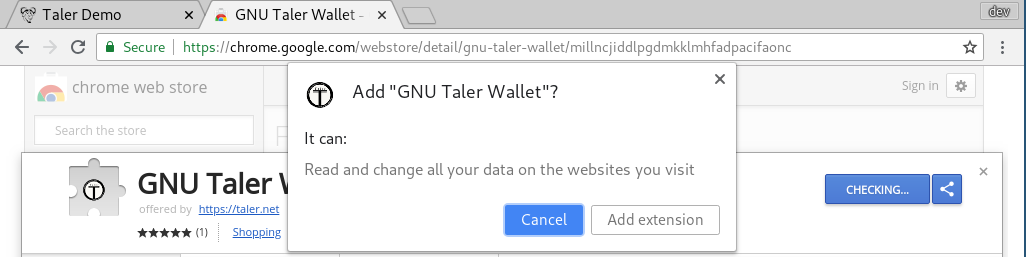
\includegraphics[width=\textwidth]{taler-screenshots/wallet-install-prompt.png}
\caption{The user is prompted to install the wallet.}
\label{fig:ux:install-prompt}
\end{figure}

\begin{figure}
\centering
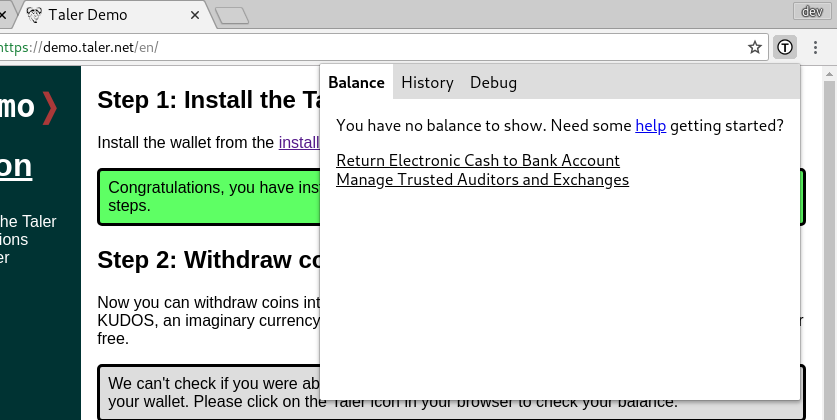
\includegraphics[width=\textwidth]{taler-screenshots/wallet-installed.png}
\caption{The wallet popup shows an empty balance.}
\label{fig:ux:installed}
\end{figure}

\begin{figure}
\centering
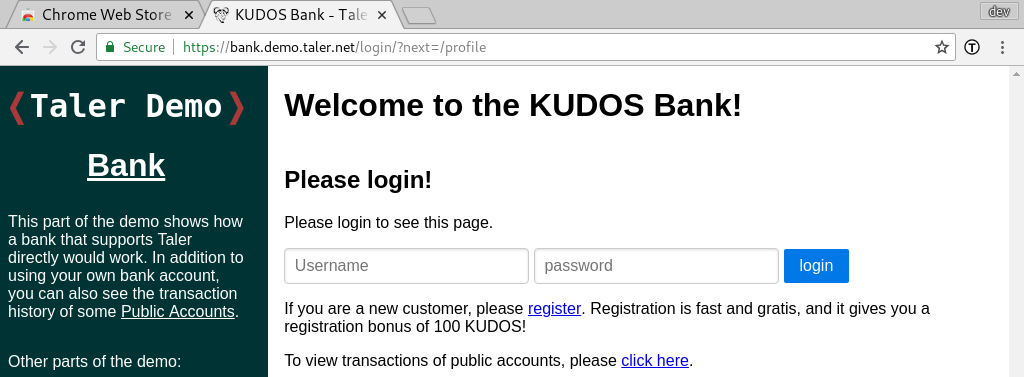
\includegraphics[width=\textwidth]{taler-screenshots/bank-login.png}
\caption{The bank asks for login details.}
\label{fig:ux:bank-login}
\end{figure}

\begin{figure}
\centering
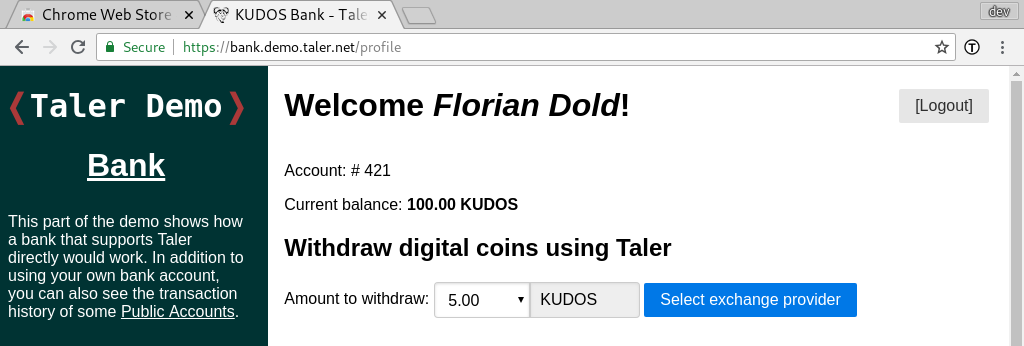
\includegraphics[width=\textwidth]{taler-screenshots/bank-profile.png}
\caption{Account page of the demo bank.}
\label{fig:ux:bank-profile}
\end{figure}

\begin{figure}
\centering
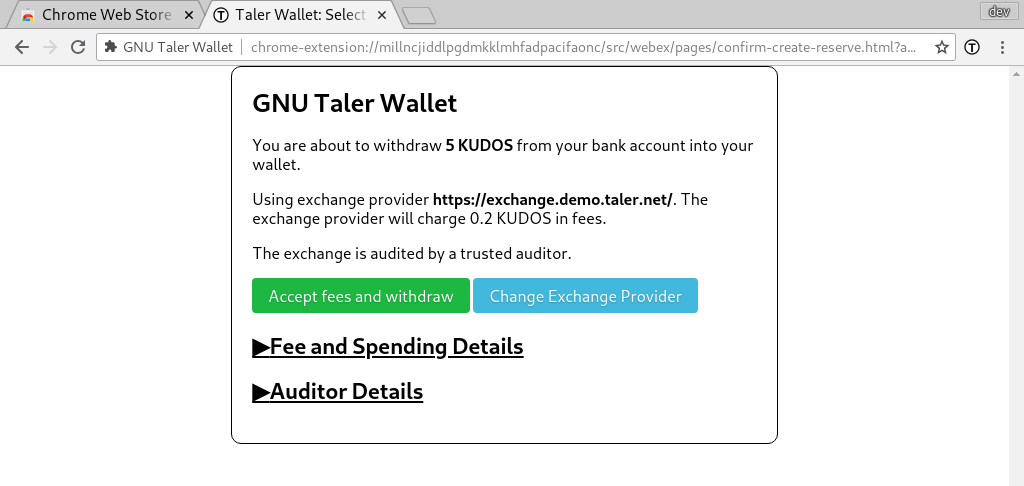
\includegraphics[width=\textwidth]{taler-screenshots/withdraw-confirm.png}
\caption{Exchange selection dialog in the wallet.}
\label{fig:ux:select-exchange}
\end{figure}

\begin{figure}
\centering
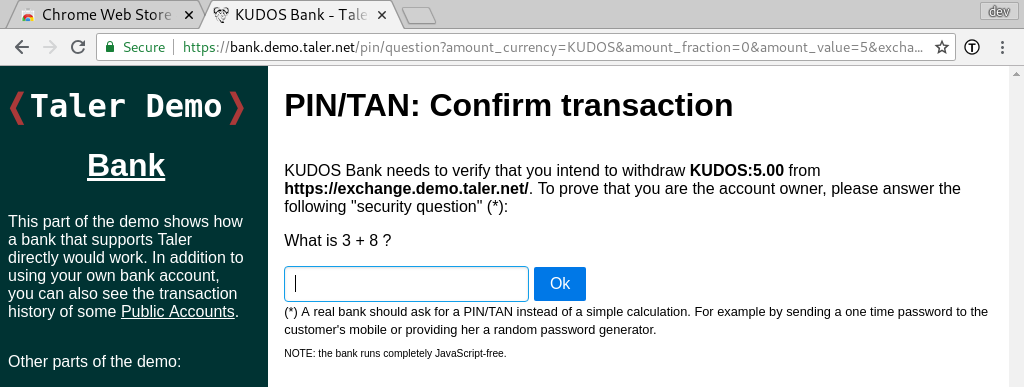
\includegraphics[width=\textwidth]{taler-screenshots/pin-tan.png}
\caption{PIN/TAN dialog of the demo bank.}
\label{fig:ux:pin-tan}
\end{figure}

\begin{figure}
\centering
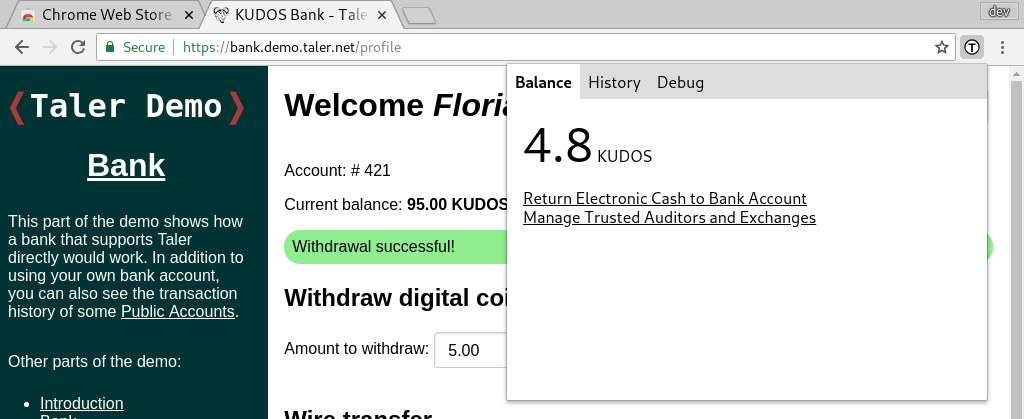
\includegraphics[width=\textwidth]{taler-screenshots/withdraw-done.png}
\caption{After a successful withdrawal, the balance is shown in the wallet.}
\label{fig:ux:withdraw-done}
\end{figure}

\begin{figure}
\centering
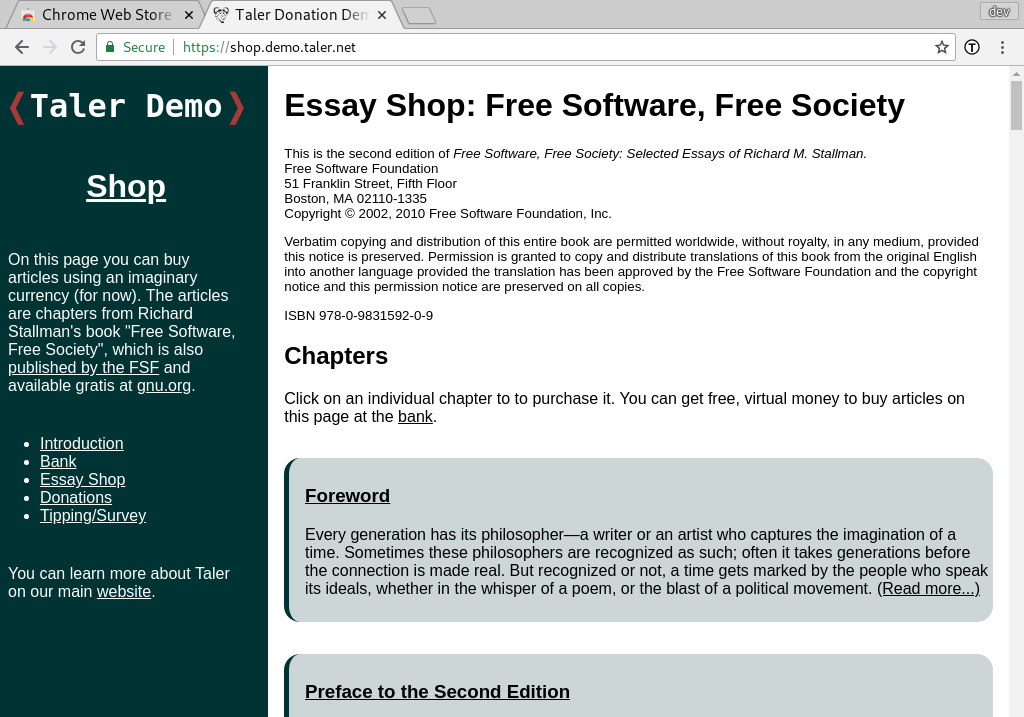
\includegraphics[width=\textwidth]{taler-screenshots/essay-landing.png}
\caption{Landing page of a store that sells essays.}
\label{fig:ux:essay-landing}
\end{figure}

\begin{figure}
\centering
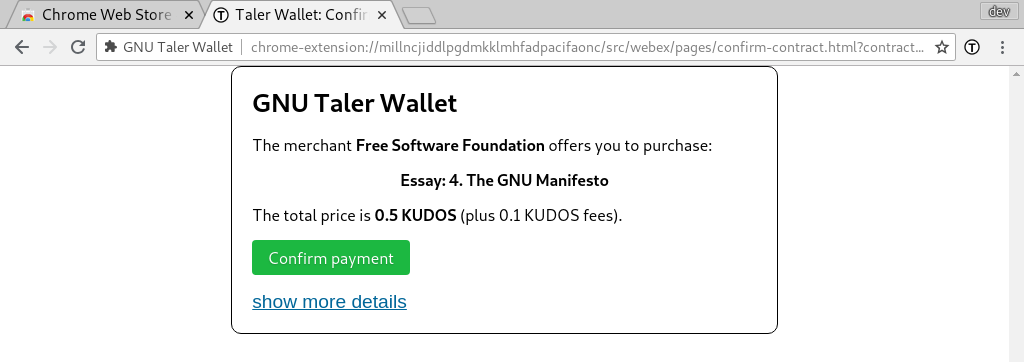
\includegraphics[width=\textwidth]{taler-screenshots/essay-pay.png}
\caption[Payment prompt for an essay.]{Payment prompt for an essay.  Rendered by the wallet.}
\label{fig:ux:essay-pay}
\end{figure}

\begin{figure}
\centering
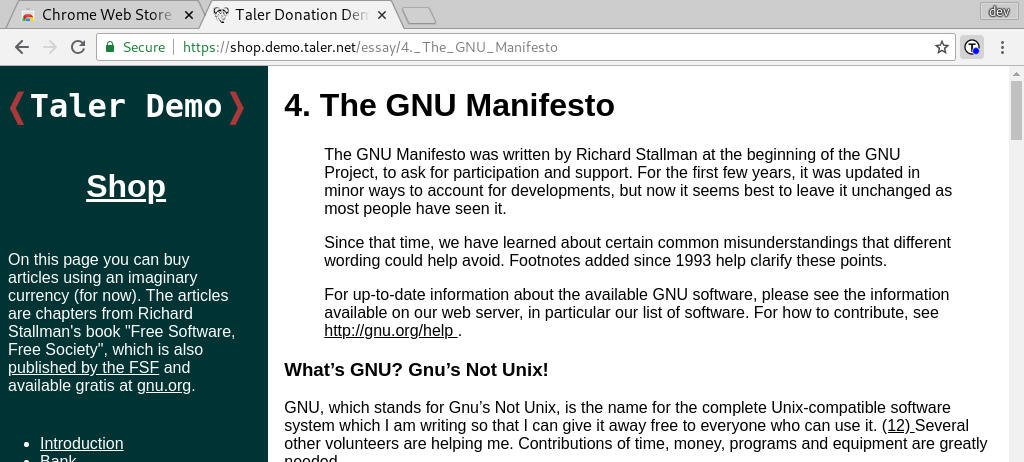
\includegraphics[width=\textwidth]{taler-screenshots/essay-done.png}
\caption{Essay successfully purchased by the user.}
\label{fig:ux:essay-done}
\end{figure}

%\begin{figure}
%\begin{subfigure}{.5\textwidth}
%  \centering
%  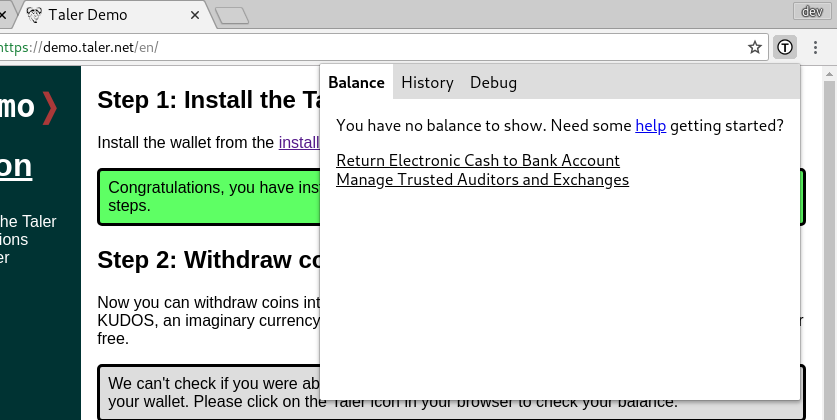
\includegraphics[width=.8\linewidth]{taler-screenshots/wallet-installed.png}
%  \caption{1a}
%  \label{fig:sfig1}
%\end{subfigure}%
%\begin{subfigure}{.5\textwidth}
%  \centering
%  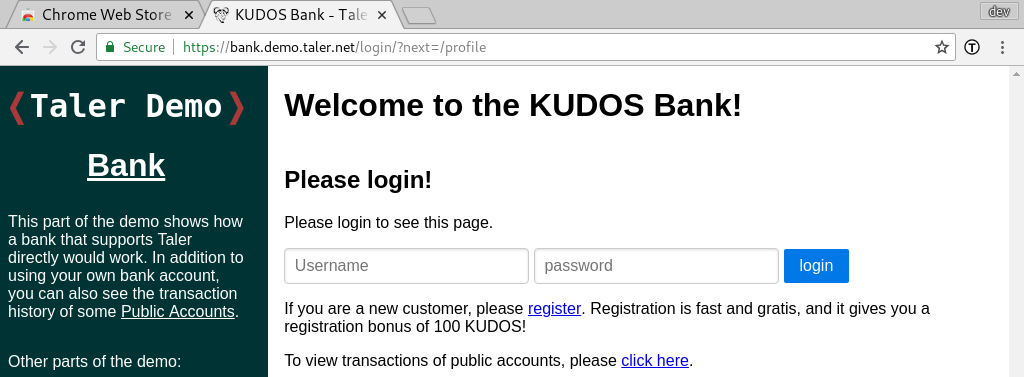
\includegraphics[width=.8\linewidth]{taler-screenshots/bank-login.png}
%  \caption{1b}
%  \label{fig:sfig2}
%\end{subfigure}
%\caption{plots of....}
%\label{fig:fig}
%\end{figure}

% FIXME: perf results

\section{The Technical Foundation: Anonymous E-Cash} \label{sec:intro:ecash}
GNU Taler is based on anonymous e-cash.  Anonymous e-cash was invented by David
Chaum in the 1980s \cite{chaum1983blind}.  The idea behind Chaumian e-cash is
both simple and ingenious, and can be best illustrated
with the carbon paper\footnote{%
  Carbon paper is a paper coated with pigment (originally carbon) on one side.
  When put face-down between two sheets of normal paper, the pressure from
  writing with a pen or typewriter on the first layer causes pigment to be
  deposited on the paper beneath, allowing a copy to be made.
} analogy:  A long, random serial number is generated, for example, by throwing
a die a few dozen times, and written on a piece of paper.  A carbon paper is
placed on top, with the pigmented side facing down, and both pieces of paper
are put into an opaque envelope.  The envelope is now sealed and brought to a
bank.  The bank draws a signature on the outside of the envelope, which presses
through to the piece of paper with the serial number.  In exchange for the
signed envelope, the bank deducts a fixed amount (say five dollars) from the
customer's bank account.  Under the (admittedly rather strong) assumption that
the bank's signature cannot be forged, the signed piece of paper with the serial
number is now an untraceable bank note worth five dollars, as the bank signed
it without seeing the serial number inside the envelope!  Since the signed
paper can be easily copied, merchants that accept it as payment must check the
bank's signature, call the bank and transmit the serial number.  The bank keeps
a register of all serial numbers that have been used as payment before.  If the
serial number is already in the bank's register, the bank informs the merchant
about the attempted double spending, and the merchant then rejects the payment.

The digital analogue of this process is called a \emph{blind signature}, where
the signer knows that it gave a digital signature, but does not know the
contents of the message that it signed.

In this document, we use \emph{coin} to refer to a token of value in an e-cash
system.  Note that the analogy of a coin does not always hold up, as certain
types of operations possible in some e-cash schemes, such as partial spending,
divisibility, etc., do not transfer to physical coins.


%\subsection{Security Properties}\label{sec:intro:security}

We have the following security and correctness properties for GNU Taler
(formally defined in Chapter~\ref{chapter:security}):
\begin{itemize}
  \item \emph{Anonymity} guarantees that transactions cannot be correlated with withdrawals or
    other transactions made by the same customer.
  \item \emph{Unforgeability} guarantees that users cannot spend more e-cash than they withdrew.
  \item \emph{Conservation} guarantees that customers do not lose money due to
    interrupted protocols or malicious merchants; they can always obtain
    anonymous change or a proof of successful spending.
  \item \emph{Income transparency} guarantees that mutually distrusting parties
    are unable to reliably transfer e-cash between them without the income of
    participants being visible to tax auditors.
\end{itemize}

While anonymity and unforgeability are common properties of e-cash, we are not
aware of any other treatments of income transparency and conservation.


\section{Roadmap}

Chapter \ref{chapter:design} describes the high-level design of GNU Taler, and
compares it to payment systems found in the academic literature and real-world
usage.  Chapter \ref{chapter:security} first gives a gentle introduction to
provable security (which can be skipped by readers with a background in
cryptography), and then defines security properties for income-transparent,
anonymous e-cash.  The cryptographic protocols for GNU Taler are defined in
detail, and proofs are given that our protocols satisfy the security
properties defined earlier.  In Chapter \ref{chapter:implementation}, the
implementation of GNU Taler is described, and the performance and scalability
is evaluated.  Chapter \ref{chapter:future-work} discusses future work and
missing pieces to deploy GNU Taler in production.  Chapter
\ref{chapter:conclusion} concludes with an outlook on the potential impact and
practical relevance of this work.



% FIXME:  maybe move things around a bit, structure it better into
% sections and subsections?

% FIXME:  talk about amounts and anonymity


\chapter{GNU Taler, an Income-Transparent Anonymous E-Cash System}\label{chapter:design}

This chapter gives a high-level overview of the design of GNU Taler, based on
the requirements discussed in Chapter~\ref{chapter:introduction}.  The
cryptographic protocols and security properties are described and analyzed in detail in
Chapter~\ref{chapter:security}.  A complete implementation with focus on of Web
payments is discussed in Chapter~\ref{chapter:implementation}.


\section{Design of GNU Taler}

GNU Taler is based on the idea of Chaumian e-cash \cite{chaum1983blind}, with
some differences and additions explained in the following sections.  Other
variants and extensions of anonymous e-cash and blind signatures are discussed in
Section~\ref{sec:related-work:e-cash}.


\subsection{Entities and Trust Model}
GNU Taler consists of the following entities (see \ref{fig:taler-arch}):
\begin{itemize}
  \item The \emph{exchanges} serve as payment service provider for a
    financial transaction between a customer and a merchant. They hold bank money
    in escrow in exchange for anonymous digital \emph{coins}.
  \item The \emph{customers} keep e-cash in their electronic \emph{wallets}.
  \item The \emph{merchants} accept digital coins in exchange for digital or physical
    goods and services.  The digital coins can be deposited with the exchange,
    in exchange for bank money.
  \item The \emph{banks} receive wire transfer instructions from customers
    and exchanges.  A customer, merchant and exchange involved in one
    GNU Taler payment do not need to have accounts with the same bank,
    as long as wire transfers can be made between the respective banks.
  \item The \emph{auditors}, typically run by trusted financial regulators,
    monitor the behavior of exchanges to assure customers and merchants that
    exchanges operate correctly.
\end{itemize}

\begin{figure}
  \begin{center}
  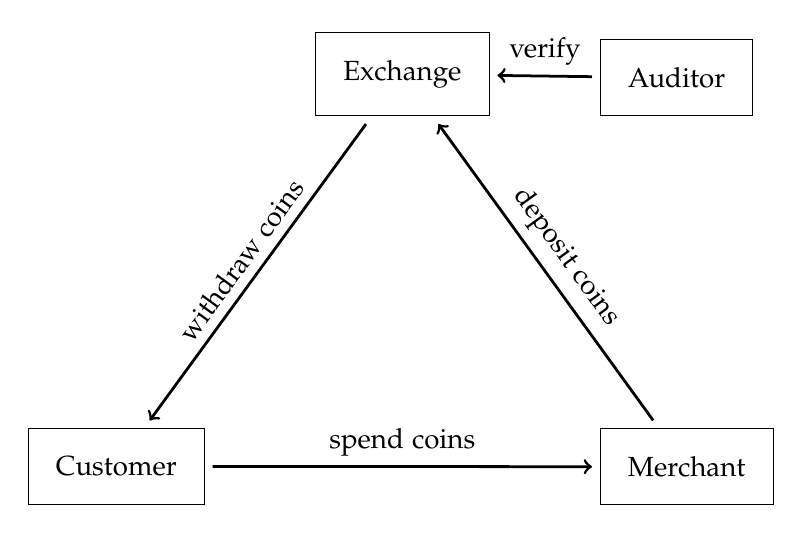
\begin{tikzpicture}
   \tikzstyle{def} = [node distance= 5em and 6.5em, inner sep=1em, outer sep=.3em];
   \node (origin) at (0,0) {};
   \node (exchange) [def,above=of origin,draw]{Exchange};
   \node (customer) [def, draw, below left=of origin] {Customer};
   \node (merchant) [def, draw, below right=of origin] {Merchant};
   \node (auditor) [def, draw, above right=of origin]{Auditor};

   \tikzstyle{C} = [color=black, line width=1pt]

   \draw [<-, C] (customer) -- (exchange) node [midway, above, sloped] (TextNode) {withdraw coins};
   \draw [<-, C] (exchange) -- (merchant) node [midway, above, sloped] (TextNode) {deposit coins};
   \draw [<-, C] (merchant) -- (customer) node [midway, above, sloped] (TextNode) {spend coins};
   \draw [<-, C] (exchange) -- (auditor) node [midway, above, sloped] (TextNode) {verify};

  \end{tikzpicture}
  \end{center}
  \caption[High-level overview of GNU Taler components.]{High-level overview of the different components of GNU Taler, banks are omitted.}
  \label{fig:taler-arch}
\end{figure}

In GNU Taler, the exchanges can be separate entities from the banks.  This fosters
competition between exchanges, and allows Taler to be deployed in an
environment with legacy banks that do not support Taler directly.

If a customer wants to pay a merchant, the customer needs to hold coins at an
exchange that the merchant trusts.  To make the selection of trusted exchanges
simpler, merchants and customers can choose to automatically trust all
exchanges audited by a certain auditor.

The exchange is trusted to hold funds of its customers in escrow and to make
payments to merchants when digital coins are deposited.  Customer and merchant
can have assurances about the exchange's liquidity and operation though the
auditor, which would typically be run by financial regulators or other trusted
third parties.

\subsection{System Assumptions}

We assume that an anonymous, bi-directional communication channel\footnote{%
An anonymization layer like Tor \cite{dingledine2004tor} can provide a
practical approximation of such a communication channel, but does not provide
perfect anonymity \cite{johnson2013users}.
} is used for
all communication between the customer and the merchant, as well as for
obtaining unlinkable change for partially spent coins from the exchange and for
retrieving the exchange's public keys used in verifying and blindly signing
coins.  The withdrawal protocol, on the other hand, does not require an
anonymous channel to preserve the anonymity of electronic coins.

During withdrawal, the exchange knows the identity of the withdrawing customer,
as there are laws, or bank policies, that limit the amount of cash that an
individual customer can withdraw in a given time
period~\cite{france2015cash,greece2015cash}.  GNU Taler is thus only anonymous with
respect to \emph{payments}.  While the exchange does know their customer (KYC),
it is unable to link the known identity of the customer that withdrew anonymous
digital coins to the \emph{purchase} performed later at the merchant.

While customers can make untraceable digital cash payments, the exchange will
always learn the merchants' identity, which is necessary to credit their
accounts.  This information can also be used for taxation, and GNU Taler
deliberately exposes these events as anchors for tax audits on merchants'
income.  Note that while GNU Taler \emph{enables} taxation, it does not
\emph{implement} any automatic taxation.

GNU Taler assumes that each participant has full control over their
system%
\footnote{%
  Full control goes both ways:  it gives the customer the freedom to run their own software,
  but also means that the behavior of fraudulent customers cannot be restricted by
  simpler technical means such as keeping balances on tamper-proof smart cards,
  and thus can lead to an overall more complex system.
}.  We assume the contact information of the exchange is known to
both customer and merchant from the start, and the customer
can authenticate the merchant, for example, by using X.509
certificates~\cite{rfc6818}.  A GNU Taler merchant is expected to deliver
the service or goods to the customer upon receiving payment.  The
customer can seek legal relief to achieve this, as the customer
receives cryptographic evidence of the contract and the associated
payment.

% FIXME:  who needs to be trusted for anonymity?

\subsection{Reserves}

A \emph{reserve} refers to a customer's non-anonymous funds at an exchange,
identified by a reserve public key.  Suppose a customer wants to convert money
into anonymized digital coins.  To do that, the customer first creates a
reserve private/public key pair, and then transfers money via their bank to the
exchange.  The wire transfer instruction to the bank must include the reserve
public key.  To withdraw coins from a reserve, the customer authenticates
themselves using the corresponding reserve private key.

Typically, each wire transfer is made with a fresh reserve public key and thus
creates a new reserve, but making another wire transfer with the same reserve
public key simply adds funds to the existing reserve.  Even after all funds
have been withdrawn from a reserve, customers should keep the reserve key pair
until all coins from the corresponding reserve have been spent, as in the event
of a denomination key revocation (see Section \ref{sec:revocation-recoup}) the
customer needs this key to recover coins of revoked denominations.

The exchange automatically transfers back to the customer's bank account any
funds that have been left in a reserve for an extended amount of time, allowing
customers that lost their reserve private key to eventually recover their
funds.  If a wire transfer to the exchange does not include a valid reserve public key,
the exchange transfers the money back to the sender.

Figure~\ref{fig:reserve:state} illustrates the state machine for a reserve.
Long-terms states are shown in boxes, while actions are in circles.  The final
state is in a double-circle.  A reserve is first {\em filled} by a wire
transfer. The amount in it is reduced by withdraw operations. If the balance
reaches zero, the reserve is {\em drained}. If a reserve is not drained after
a certain amount of time, it is automatically closed.  A reserve can also be
filled via a recoup action (see Section~\ref{sec:revocation-recoup}) in case
that the denomination of an unspent coin that was withdrawn from the reserve
is revoked.

\begin{figure}
  \begin{center}
    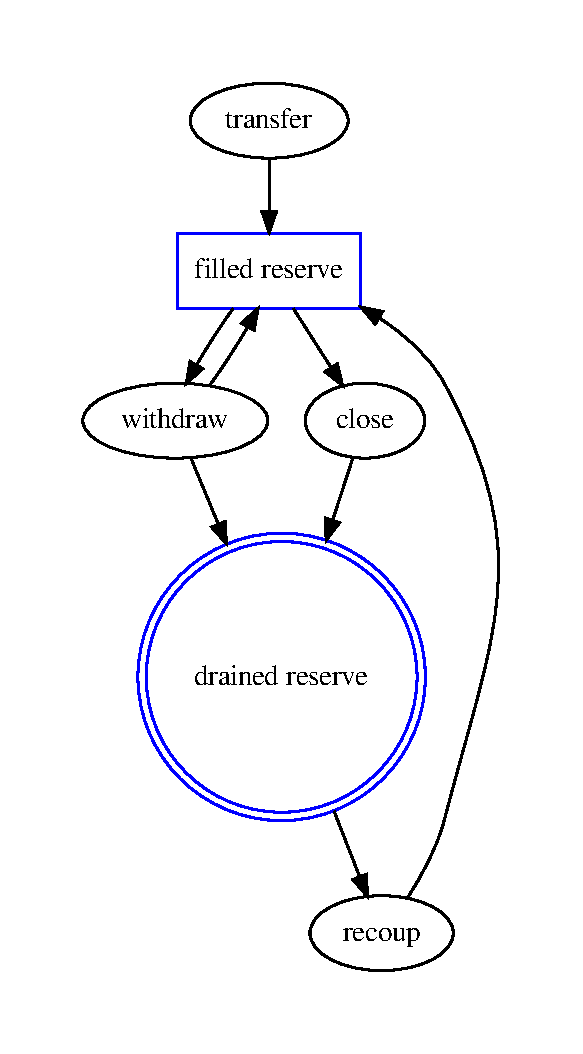
\includegraphics{taler/reserve.pdf}
  \end{center}
  \caption{State machine of a reserve.}
  \label{fig:reserve:states}
\end{figure}

Instead of requiring the customer to manually generate reserve key pairs and
copy them onto a wire transfer form, banks can offer tight integration with the
GNU Taler wallet software.  In this scenario, the bank's website or banking app
provides a ``withdraw to GNU Taler wallet'' action.  After selecting this
action, the user is asked to choose the amount to withdraw from their bank
account into the wallet.  The bank then instructs the GNU Taler wallet software
to create record of the corresponding reserve; this request contains the anticipated amount, the
reserve key pair and the URL of the exchange to be used.  When invoked by the
bank, the wallet asks the customer to select an exchange and to confirm the
reserve creation.  The exchange chosen by the customer must support the wire
transfer method used by the bank, which will be automatically checked by the
wallet.  Typically, an exchange is already selected by default, as banks can
suggest a default exchange provider to the wallet, and additionally wallets
have a pre-defined list of trusted exchange providers.  Subsequently, the wallet
hands the reserve public key and the bank account information of the selected
exchange back to the bank.  The bank---typically after asking for a second authentication
factor from the customer---will then trigger a wire transfer to the exchange with
the information obtained from the wallet.

When the customer's bank does not offer tight integration with GNU Taler, the
customer can still manually instruct their wallet to create a reserve.  The public
key must then be included in a bank transaction to the exchange.  When the
customer's banking app supports pre-filling wire transfer details from a URL or
a QR code, the wallet can generate such a URL or QR code that includes the
pre-filled bank account details of the exchange as well as the reserve public
key.  The customer clicks on this link or scans the QR code to invoke their
banking app with pre-filled transaction details.  Since there currently is no
standardized format for pre-filled wire transfer details, we are proposing the
\texttt{payto://} URI format explained in
Section~\ref{implementation:wire-method-identifiers}, currently under review
for acceptance as an IETF Internet Standard.


% FIXME: withdrawal strategy, coin selection

\subsection{Coins and Denominations}

Unlike plain Chaumian e-cash, where a coin just contains a serial number, a
\emph{coin} in Taler is a public/private key pair where the private key is only
known to the owner of the coin.

A coin derives its financial value from a blind signature on the coin's
public key. The exchange has multiple \emph{denomination key} pairs available
for blind-signing coins of different financial values.  Other approaches for representing
different denominations are discussed in Section~\ref{design:related-different-denominations}.

Denomination keys have an expiration date, before which any coins signed with
it must be spent or exchanged into newer coins using the refresh protocol
explained in Section \ref{sec:design-refresh}.  This allows the exchange to
eventually discard records of old transactions, thus limiting the records that
the exchange must retain and search to detect double-spending attempts.  If a
denomination's private key were to be compromised, the exchange can detect this
once more coins are redeemed than the total that was signed into existence
using that denomination key.  Should such an incident occur, the exchange can allow authentic
customers to redeem their unspent coins that were signed with the compromised
private key, while refusing further deposits involving coins signed by the
compromised denomination key (see Section~\ref{sec:revocation-recoup}).  As a result, the
financial damage of losing a private signing key is limited to at most the
amount originally signed with that key, and denomination key rotation can be
used to bound that risk.

To prevent the exchange from deanonymizing users by signing each coin with a
fresh denomination key, exchanges publicly announce their denomination keys
in advance with validity periods that imply sufficiently strong anonymity sets.
These announcements are expected to be signed with an offline long-term
private \emph{master signing key} of the exchange and the auditor.
Customers should obtain these announcements using an anonymous
communication channel.

After a coin is issued, the customer is the only entity that knows the
private key of the coin, making them the \emph{owner} of the coin.  Due
to the use of blind signatures, the exchange does not learn the
public key during the withdrawal process.  If the private key is
shared with others, they become co-owners of the coin.  Knowledge of
the private key of the coin and the signature over the coin's public
key by an exchange's denomination key enables spending the
coin.

\subsection{Partial Spending and Unlinkable Change}

Customers are not required to have exact change ready when making a payment.
In fact, it should be encouraged to withdraw a larger amount of e-cash
beforehand, as this blurs the correlation between the non-anonymous withdrawal
event and the anonymous spending event, increasing the anonymity set.

A customer spends a coin at a merchant by cryptographically signing a
\emph{deposit permission} with the coin's private key.  A deposit permission
contains the hash of the \emph{contract terms}, i.e., the details of the
purchase agreement between the customer and merchant. Coins can be
\emph{partially} spent, and a deposit permission specifies the fraction of the
coin's value to be paid to the merchant. As digital coins are trivial to copy,
the merchant must immediately deposit them with the exchange, in order to get a
deposit confirmation or an error that indicates double spending.

When a coin is used in a completed or attempted/aborted payment, the coin's
public key is revealed to the merchant/exchange, and further payments with the
remaining amount would be linkable to the first spending event.  To obtain
unlinkable change for a partially spent (or otherwise revealed coin), GNU
Taler introduces the \emph{refresh protocol}, which consists of three steps:
\emph{melt}, \emph{reveal} and \emph{link}.  The refresh protocol allows the
customer to obtain new coins for the remaining amount on a coin.  The old coin
is marked as spent after it has been melted, while the reveal step generates
the fresh coins.  Using blind signatures to withdraw the refreshed coins makes
them unlinkable from the old coin.

% FIXME: talk about logarithmic time, simulation

\subsection{Refreshing and Taxability}\label{sec:design-refresh}
% FIXME:  maybe put section on how to avoid withdraw loophole here!
One goal of GNU Taler is to make merchants' income transparent to state auditors,
so that income can be taxed appropriately.  Naively implemented, however, a simple
refresh protocol could be used to evade taxes:  the payee of an untaxed
transaction would generate the private keys for the coins that result from
refreshing a (partially spent) old coin, and send the corresponding public keys
to the payer.  The payer would execute the refresh protocol, provide the
payee's coin public keys for blind signing, and provide the signatures to the
payee, who would now have exclusive control over the coins.

To remedy this, the refresh protocol introduces a \emph{link threat}: coins are
refreshed in such a way that the owner of the old coin can always obtain the
private key and exchange's signature on the new coins resulting from refreshes,
using a separate \emph{linking protocol}.  This introduces a threat to
merchants that try to obtain untaxed income.  Until the coins are finally
deposited at the exchange, the customer can always re-gain ownership of them
and could deposit them before the merchant gets a chance to do so.  This
disincentivizes the circulation of unreported income among untrusted parties in
the system.

In our implementation of the refresh and linking protocols, there is a
non-negligible success chance ($\frac{1}{\kappa}$, depending on system parameter
$\kappa$, typically $\ge 3$) for attempts to cheat during the refresh protocol,
resulting in refreshed coins that cannot be recovered from the old coin via the
linking protocol.  Cheating during refresh, however, is still not
\emph{profitable}, as an unsuccessful attempt results in completely losing the
amount that was intended to be refreshed.

% FIXME:  mention that we don't want to use DRM/HSMs for this

For purposes of anti-money-laundering and taxation, a more detailed audit of
the merchant's transactions can be desirable.  A government tax authority can
request the merchant to reveal the business agreement details that match the
contract terms hash recorded with the exchange.  If a merchant is not able to
provide theses values, they can be subjected to financial penalties by the
state in relation to the amount transferred by the traditional currency
transfer.

\subsection{Transactions vs. Sharing}

Sharing---in contrast to a transaction---happens when mutually trusted parties
simultaneously have access to the private keys and signatures on coins.
Sharing is not considered a transaction, as subsequently both parties have equal control
over the funds.  A useful application for sharing are peer-to-peer payments
between mutually trusting parties, such as families and friends.

\subsection{Aggregation}

For each payment, the merchant can specify a deadline before which the exchange
must issue a wire transfer to the merchant's bank account.  Before this
deadline occurs, multiple payments from deposited coins to the same merchant
can be \emph{aggregated} into one bigger payment.  This reduces transaction
costs from underlying banking systems, which often charge a fixed fee per
transaction.  To incentivize merchants to choose a longer wire transfer
deadline, the exchange can charge the merchant a fee per aggregated wire
transfer.

Figure~\ref{fig:deposit:states} illustrates the state machine for processing
deposits.  Long-terms states are shown in boxes, while actions are in circles.
The final state is in a double-circle.  Dashed arrows show transitions based
on timing and not external actions. A deposit is first {\em created} when a
wallet makes a payment.  A deposit comes with a {\em refund deadline}, and the
wire transfer must not happen before that deadline. Once the refund deadline
has passed, the deposit becomes {\em ready}.  Even if a deposit is ready, it
is not automatically wired. In fact, deposits may still be {\em refunded} in
this state.  A refund may be full (resulting in the deposit being {\em done})
or partial, in which case the remaining value is left in the same deposit
state. A deposit comes with a second deadline, the {\em wire deadline}. Once
that deadline has passed, the deposit is {\em due} and must be {\em
  aggregated}.  Aggregation combines {\bf all} deposits that are {\em due},
{\em tiny} or {\em ready} into one wire transfer.  However, the amount of even
an aggregated deposit may be too small to be executed by the banking
system. In this case, the deposit transitions into the special state {\em
  tiny} until the aggregated amount meets the amount threshold.  Once
aggregated, the deposits are {\em done}.  A wire transfer is first prepared
and then {\em pending}. The transfer is {\em finished} once the bank has
confirmed the {\em transfer}.

\begin{figure}
  \begin{center}
    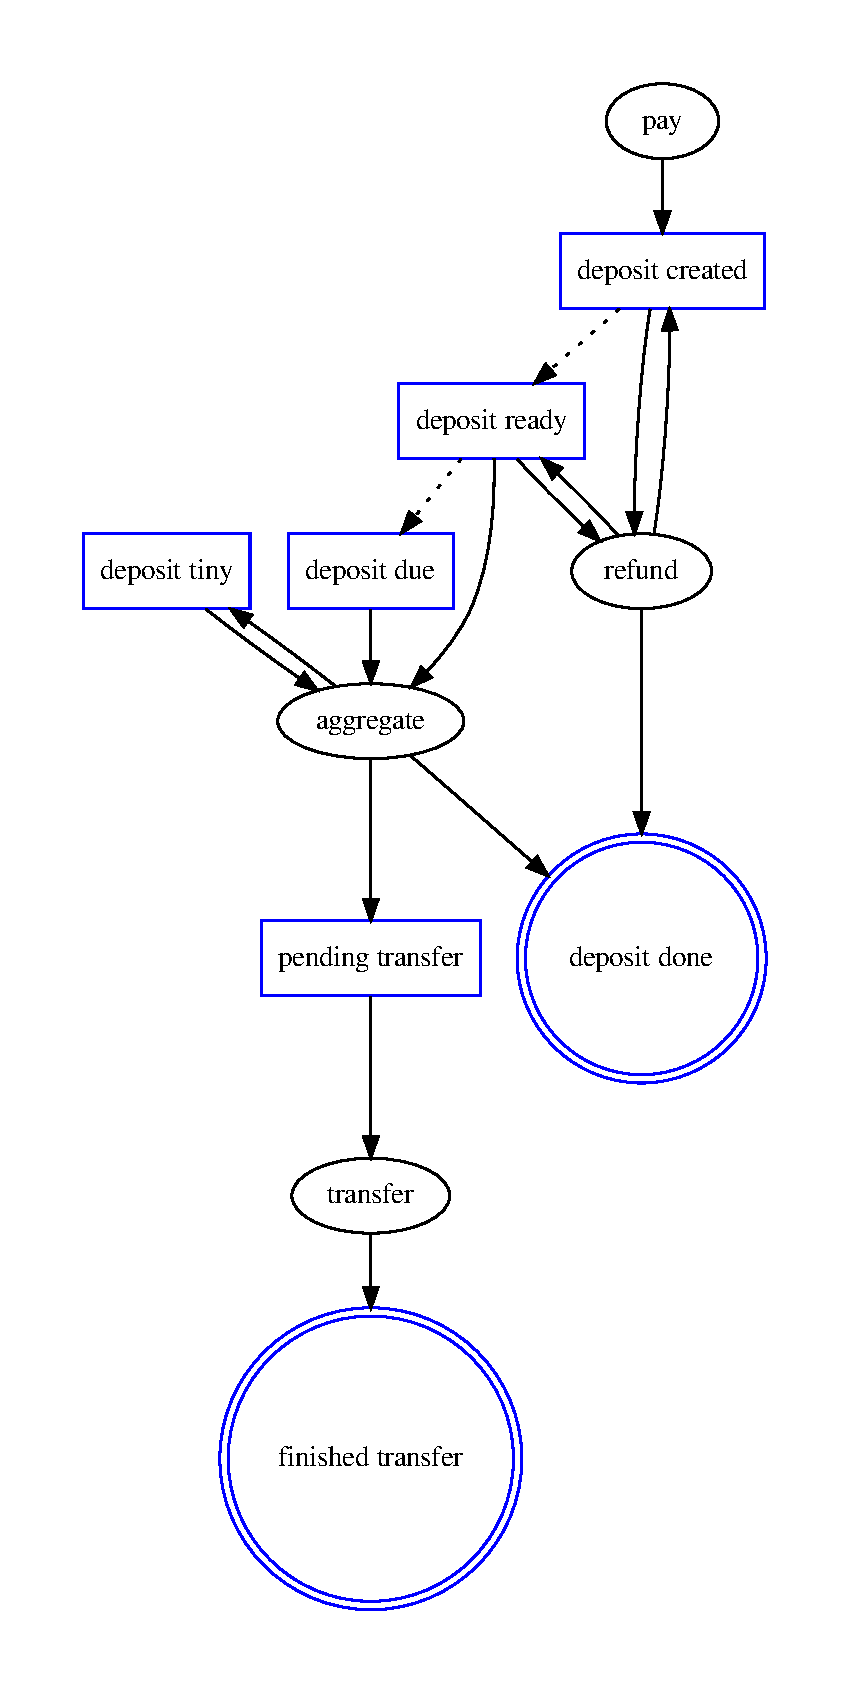
\includegraphics[scale=0.8]{taler/deposit.pdf}
  \end{center}
  \caption{State machine of a deposit.}
  \label{fig:deposit:states}
\end{figure}


\subsection{Refunds}

The aggregation period also opens the opportunity for cheap \emph{refunds}.  If
a customer is not happy with their product, the merchant can instruct the
exchange to give the customer a refund before the wire transfer deadline has
occurred.  This effectively ``undoes'' the deposit of the coin, and restores the
available amount left on it.  The refresh protocol is then used by the customer
on the coins involved in a refund, so that payments remain unlinkable.

% FIXME: mention EU customer laws / 14 weeks?

\subsection{Fees}

In order to subsidize the operation of the exchange and enable a sustainable
business model, the exchange can charge fees for most operations.  For
withdrawal, refreshing, deposit and refunds, the fee is dependent on the denomination,
as different denominations might have different key sizes, security and storage
requirements.

Most payment systems hide fees from the customer by putting them to the merchant.
This is also possible with Taler.  As different exchanges (and denominations)
can charge different fees, the merchant can specify a maximum amount of fees it
is willing to cover.  Fees exceeding this amount must be explicitly paid by the
customer.

Another consideration for fees is the prevention of denial-of-service attacks.
To make ``useless'' operations, such as repeated refreshing on coins
(causing the exchange to use relatively expensive storage), unattractive to an
adversary, these operations must charge a fee.  Again, for every refresh
following a payment, the merchant can cover the costs up to a limit set by the
merchant, effectively hiding the fees from the customer.

Yet another type of fee are the \emph{wire transfer fees}, which are charged
by the exchange for every wire transfer to a merchant in order to compensate for
the cost of making a transaction in the underlying bank system.  The wire
transfer fees encourage merchants to choose longer aggregation periods, as the
fee is charged per transaction and independant of the amount.

Merchants can also specify the maximum wire fee they are willing to cover for
customers, along with an \emph{amortization rate} for the wire fees.  In case
the wire fees for a payment exceed the merchant's chosen maximum, the customer
must additionally pay the excess fee divided by the amortization rate.  The
merchant should set amortization rate to the expected number of transactions
per wire transfer aggregation window.  This allows the merchant to adjust
the total expected amount that it needs to pay for wire fees.


\subsection{The Withdraw Loophole and Tipping}\label{taler:design:tipping}

The withdraw protocol can be (ab)used to illicitly transfer money, when the
receiver generates the coin's secret key, and gives the public key to the party
executing the withdraw protocol.  We call this the ``withdraw loophole''.  This
is only possible for one ``hop'', as money can still not circulate among
mutually distrusted parties, due to the properties of the refresh protocol.

A ``benevolent'' use of the withdraw loophole is \emph{tipping}, where merchants give
small rewards to customers (for example, for filling out a survey or installing
an application), without any contractual obligations or digitally signed
agreement.

% FIXME:  argue that this can't be done on scale for money laundering

\subsubsection{Fixing the Withdraw Loophole}\label{taler:design:fixing-withdraw-loophole}

In order to discourage the usage of the withdraw loophole for untaxed payments,
the following approach would be possible:  Normal withdraw operations and
unregistered reserves are disabled, except for special tip reserves that are
registered by the merchant as part of a tipping campaign.  Customers are
required to pre-register at the exchange and obtain a special withdraw key pair
against a small safety deposit.  Customer obtain new coins via a refresh
operation from the withdraw key to a new coin.  If customers want to abuse
Taler for untaxed payments, they either need to risk losing money by lying
during the execution of the refresh protocol, or share their reserve private
key with the payee.  In order to discourage the latter, the exchanges gives the
safety deposit to the first participant who reports the corresponding private
key as being used in an illicit transaction, and requires a new safety deposit
before the customer is allowed to withdraw again.

However since the withdraw loophole allows only one additional ``payment'' (without any
cryptographic evidence that can be used in disputes) before the coin must be deposited,
these additional mitigations might not even be justified considering their additional cost.


\section{Auditing}
The auditor is a component of GNU Taler which would typically be deployed by a
financial regulator, fulfilling the following functionality:
\begin{itemize}
  \item It regularly examines the exchange's database and
    bank transaction history to detect discrepancies.
  \item It accepts samples of certain protocol responses that merchants
    received from an audited exchange, to verify that what the exchange signed
    corresponds to what it stored in its database.
  \item It certifies exchanges that fulfill the operational and financial requirements
    demanded by regulators.
  \item It regularly runs anonymous checks to ensure that the required protocol
    endpoints of the exchange are available.
  \item In some deployment scenarios, merchants need to pre-register with exchanges to fulfill know-your-customer (KYC) requirements.
    The auditor provides a list of certified exchanges to merchants,
    to which the merchant then can automatically KYC-register.
  \item It provides customers with an interface to submit cryptographic proof that an exchange
    misbehaved.  If a customer claims that the exchange denies service, it can execute a request on
    behalf of the customer.
\end{itemize}

%An exchange operator would typically run their own instance of the auditor software,
%to ensure correct operation.

% FIXME: live auditing

% FIXME: discuss indian merchant scenario

\subsection{Exchange Compromise Modes}

The exchange is an attractive target for hackers and insider threats.  We now
discuss different ways that the exchange can be compromised, how to reduce the
likelihood of such a compromise, and how to detect and react to such an event
if it happens.

\subsubsection{Compromise of Denomination Keys and Revocation}\label{sec:revocation-recoup}

When a denomination key pair is compromised, an attacker can ``print money'' by
using it to sign coins of that denomination.  An exchange (or its auditor) can
detect this when the number of deposits for a certain denomination exceed the
number of withdrawals for that same denomination.

We allow the exchange to revoke denomination keys, and wallets periodically
check for such revocations.  We call a coin of a revoked denomination a revoked
coin.  If a denomination key has been revoked, the wallets use the
\emph{recoup} protocol to recover funds from coins of revoked denominations.
Once a denomination is revoked, new coins of this denomination can't be
withdrawn or used as the target denomination for a refresh operation. A revoked
coin cannot be spent, and can only be refreshed if its public key was recorded
in the exchange's database (as spending/refresh operations) before it was
revoked.

The following cases are possible for recoup:
\begin{enumerate}
  \item The revoked coin has never been seen by the exchange before, but the
    customer can prove via a withdraw protocol transcript and blinding factor
    that the coin resulted from a legitimate withdrawal from a reserve.  In
    this case, the exchange credits the reserve that was used to withdraw the
    coin with the value of the revoked coin.
  \item The coin has been partially spent.  In this case, the exchange allows
    the remaining amount on the coin to be refreshed into fresh coins of
    non-revoked denominations.
  \item The revoked coin $C_R$ has never been seen by the exchange before, was
    obtained via the refresh protocol, and the exchange has an existing record
    of either a deposit or refresh for the ancestor coin $C_A$ that was
    refreshed into the revoked coin $C_R$. If the customer can prove this by
    showing a corresponding refresh protocol transcript and blinding factors, the exchange credits
    the remaining value of $C_R$ on $C_A$.  It is explicitly permitted for $C_A$
    to be revoked as well.  The customer can then obtain back their funds by
    refreshing $C_A$.
\end{enumerate}

These rules limit the maximum financial damage that the exchange can incur from
a compromised denomination key $D$ to $2nv$, with $n$ being the
maximum number of $D$-coins simultaneously in circulation and $v$ the financial
value of a single $D$-coin.  Say denomination $D$ was withdrawn by
legitimate users $n$ times.  As soon as the exchange sees more
than $n$ pairwise different $D$-coins, it must immediately
revoke $D$.  An attacker can thus at most gain $nv$ by either
refreshing into other non-revoked denominations or spending the forged $D$-coins.
The legitimate users can then request a recoup for their coins, resulting in
a total financial damage of at most $2nv$.

With one rare exception, the recoup protocol does not negatively impact the
anonymity of customers.  We show this by looking at the three different cases
for recoup on a revoked coin.  Specifically, in case (1), the coin obtained
from the credited reserve is blindly signed, in case (2) the refresh protocol
guarantees unlinkability of the non-revoked change, and in case (3) the revoked
coin $C_R$ is assumed to be fresh.  If $C_R$ from case (3) has been seen by a
merchant before in an aborted/unfinished transaction, this transaction would be
linkable to transactions on $C_A$.  Thus, anonymity is not preserved when an
aborted transaction coincides with revoked denomination, which should be rare
in practice.

Unlike most other operations, the
recoup protocol does not incur any transaction fees. The primary use of the
protocol is to limit the financial loss in cases where an audit reveals that
the exchange's private keys were compromised, and to automatically pay back
balances held in a customers' wallet if an exchange ever goes out of business.

To limit the damage of a compromise, the exchange can employ a hardware
security module that contains the denomination secret keys, and is
pre-programmed with a limit on the number of signatures it can produce.  This
might be mandated by certain auditors, who will also audit the operational
security of an exchange as part of the certification process.



\subsubsection{Compromise of Signing Keys}

When a signing key is compromised, the attacker can pretend to be a
merchant and forge deposit confirmations.  To forge a deposit
confirmation, the attacker also needs to get a customer to sign a
contract from the adversary (which should include the adversary's
banking details) with a valid coin.  The attack here is that the
customer is allowed to have spent the coin already. Thus, a deposit of
the resulting deposit permission would result in a rejection from the
exchange due to double spending.  By forging the deposit confirmation
using the compromised signing key, the attacker can thus claim in
court that they properly deposited the coin first and demand payment
from the exchange.

We note that indeed an evil exchange could simply fail to record
deposit permissions in its database and then fail to execute them.
Thus, given a merchant presenting a deposit confirmation, we need
a way to establish whether this is a case of an evil exchange that
should be compelled to pay, or a case of a compromised signing key
and where payouts (and thus financial damage to the exchange)
can legitimately be limited.

To limit the financial damage of a compromised signing key, merchants
must be required to work with auditors to perform a
\emph{probabilistic deposit auditing} of the exchange.  Here, the goal
is to help detect the compromise of a signing key by making sure that
the exchange does indeed properly record deposit confirmations.
However, double-checking with the auditor if every deposit
confirmation is recorded in the exchange's database would be too
expensive and time-consuming.  Fortunately, a probabilistic method
where merchants only send a small fraction of their deposit
confirmations to the auditor suffices.  Then, if the auditor sees a
deposit confirmation that is not recorded in the exchange's database
(possibly after performing the next synchronization with the
exchange's database), it signals the exchange that the signing key has
been compromised.

At this point, the signing key must be revoked and the exchange will
be required to investigate the security of its systems and address the
issue before resuming normal operations.
%
%If the exchange had separate short-term signing keys just for signing deposit
%confirmations, it could also employ hardware security modules with a counter,
%and check if the value of the counter matches matches the deposit confirmations
%recorded in the database.

Still, at this point various actors (including the attacker) could still
step forward with deposit confirmations signed by the revoked key and
claim that the exchange owes them for their deposits.  Simply revoking
a signing key cannot lift the exchange's payment obligations, and the
attacker could have signed an unlimited number of such deposit confirmations
with the compromised key.  However, in contrast to honest merchants, the
attacker will not have participated {\em proportionally} in the auditor's
probabilistic deposit auditing scheme for those deposit confirmations:
in that case, the key compromise would have been detected and the key
revoked.

The exchange must still pay all deposit permissions it signed for
coins that were not double-spent.  However, for all coins where
multiple merchants claim that they have a deposit confirmation, the
exchange will pay the merchants proportionate to the fraction of the
coins that they reported to the auditor as part of probabilistic
deposit auditing.  For example, if 1\% of deposits must be reported to
the auditor according to the protocol, a merchant might be paid at
most say 100+X times the number of reported deposits where $X>0$
serves to ensure proper payout despite the probabilistic nature of the
reporting.  As a result, honest merchants have an {\em incentive} to
correctly report the deposit confirmations to the auditor.

Given this scheme, the attacker can only report a small number of
deposit confirmations to the auditor before triggering the signing key
compromise detection.  Suppose again that 1\% of deposit confirmations
are reported by honest merchants, then the attacker can only expect to
submit 100 deposit permissions created by the compromised signing key
before being detected.  The attacker's expected financial benefit from
the key compromise would then be the value of $(100+X) \cdot 100$
deposit permissions.

Thus, the financial benefit to the attacker can be limited by
probabilistic deposit auditing, and honest merchants have proper
incentives to participate in the process.

\subsubsection{Compromise of the Database}

If an adversary would be able to modify the exchange, this would be detected
rather quickly by the auditor, provided that the database has appropriate
integrity mechanisms.  An attacker could also prevent database updates to block
the recording of spend operations, and then double spend.  This is effectively
equivalent to the compromise of signing keys, and can be detected with the same
strategies.

\subsubsection{Compromise of the Master Key}

If the master key was compromised, an attacker could de-anonymize customers by
announcing different sets of denomination keys to each of them.  If the
exchange was audited, this would be detected quickly, as these denominations
will not be signed by auditors.

\subsection{Cryptographic Proof}

We use the term ``proof'' in many places as the protocol provides cryptographic
proofs of which parties behave correctly or incorrectly. However,
as~\cite{fc2014murdoch} point out, in practice financial systems need to
provide evidence that holds up in courts.  Taler's implementation is designed
to export evidence and upholds the core principles described
in~\cite{fc2014murdoch}.  In particular, in providing the cryptographic proofs
as evidence none of the participants have to disclose their core secrets.

\subsection{Perfect Crime Scenarios}\label{sec:design:blackmailing}
GNU Taler can be slightly modified to thwart blackmailing or kidnapping
attempts by criminals who intend to use the anonymity properties of the system
and demand to be paid ransom in anonymous e-cash.

Our modification incurs a slight penalty on the latency for customers during normal use and
requires slightly more data to be stored in the exchange's database, and thus
should only be used in deployments where resistance against perfect crime
scenarios is necessary.  A payment system for a school cafeteria likely does
not need these extra measures.

The following modifications are made:
\begin{enumerate}
  \item Coins can now only be used in either a transaction or in a refresh operations, not a mix of both.
    Effectively, the customer's wallet then needs to use the refresh protocol to prepare exact change
    before a transaction is made, and that transaction is made with exact change.

    This change is necessary to preserve anonymity in face of the second modification, but increases
    storage requirements and latency.
  \item The recoup protocol is changed so that a coin obtained
    via refreshing must be recovered differently when revoked: to recover a revoked coin
    obtained via refreshing, the customer needs to show the transcripts for the
    chain of all refresh operations and the initial withdrawal operation
    (including the blinding factor).  Refreshes on revoked coins are not
    allowed anymore.
\end{enumerate}

After an attacker has been paid ransom, the exchange simply revokes all currently offered denominations
and registers a new set of denomination with the auditor.
Reserves used to pay the attacker are marked as blocked in the exchange's
database.  Normal users can use the recoup protocol to obtain back the money
they've previously had in revoked denominations.  The attacker can try to
recover funds via the (now modified) recoup protocol, but this attempt will
not be successful, as the initial reserve is blocked.  The criminal could also
try to spend the e-cash anonymously before it is revoked, but this is likely
difficult for large amounts, and furthermore due to income transparency all
transactions made between the payment of the ransom and the revocation can be
traced back to merchants that might be complicit in laundering the ransom
payment.

Honest customers can always use the recoup protocol to transfer the funds to
the initial reserve.  Due to modification (1), unlinkability of transactions is
not affected, as only coins that were purely used for refreshing can now be
correlated.

We believe that our approach is more practical than the approaches based on
tracing, since in a scheme with tracing, the attacker can always ask for a
plain blind signature.  With our approach, the attacker will always lose funds
that they cannot immediately spend.  Unfortunately our approach is limited to a
kidnapping scenario, and not applicable in those blackmail scenarios where the
attacker can do damage after they find out that their funds have been erased.

\subsection{Summary}

Figure~\ref{fig:coin:states} illustrates the overall state machine for processing
coins.  Long-terms states are shown in boxes, while actions are in circles.
The final state is in a double-circle.  Dashed arrows show transitions based
on timing and not external actions. The red arrow shows an action that is
allowed by the exchange but should never be done by wallets as it would
break unlinkability.

A coin begins as an unsigned {\em planchet}, which is either signed as part of
the {\em withdraw} protocol or the refresh protocol. The most common scenario
is that the {\em fresh coin} is {\em deposited}. This payment creates a
deposit (see Figure~\ref{fig:deposit:states}) and either a {\em dirty coin}
(if the payment was for a fraction of the coin's value) or a {\em spent coin}.
A spent coin can be {\em refunded} by the merchant (until the deposit is due),
creating a {\em dirty coin}.

A {\em fresh coin} may also be subject to key {\em revocation}, at which point
the wallet ends up with a {\em revoked coin}.  At this point, the wallet can
use the {\em recoup} protocol to recover the value of the coin.  If the coin
originated from a {\em withdraw} operation, the value is added back into the
reserve, which is {\em filled} in the process (see
Figure~\ref{fig:reserve:states}).  If the coin originated from the {\em
  refresh} operation, this results in the old coin turning into a {\em zombie
  coin}, which can be refreshed again.

Dirty coins and fresh coins can be {\em melted}.  Dirty coins should always be
melted automatically by the wallet as soon as possible as this is the only
good way to use them while preserving unlinkability.  A wallet should also
automatically {\em melt} any {\em fresh coins} that are in danger of their
denomination key nearing its (deposit) {\em expiration} time. If a wallet
fails to do so, coins may {\em expire}, resulting in a loss for the coin's
owner.  Dirty coins can also expire. In practice, this happens if the melt fee
exceeds the residual value of the dirty coin.  To {\em melt} a coin, the
wallet must commit to one or more {\em planchets} and then demonstrate honesty
when the committment made for the {\em refresh session} is checked during the
{\em reveal} step. If the wallet was honest, {\em reveal} yields {\em fresh
  coins}.

\begin{figure}
  \begin{center}
    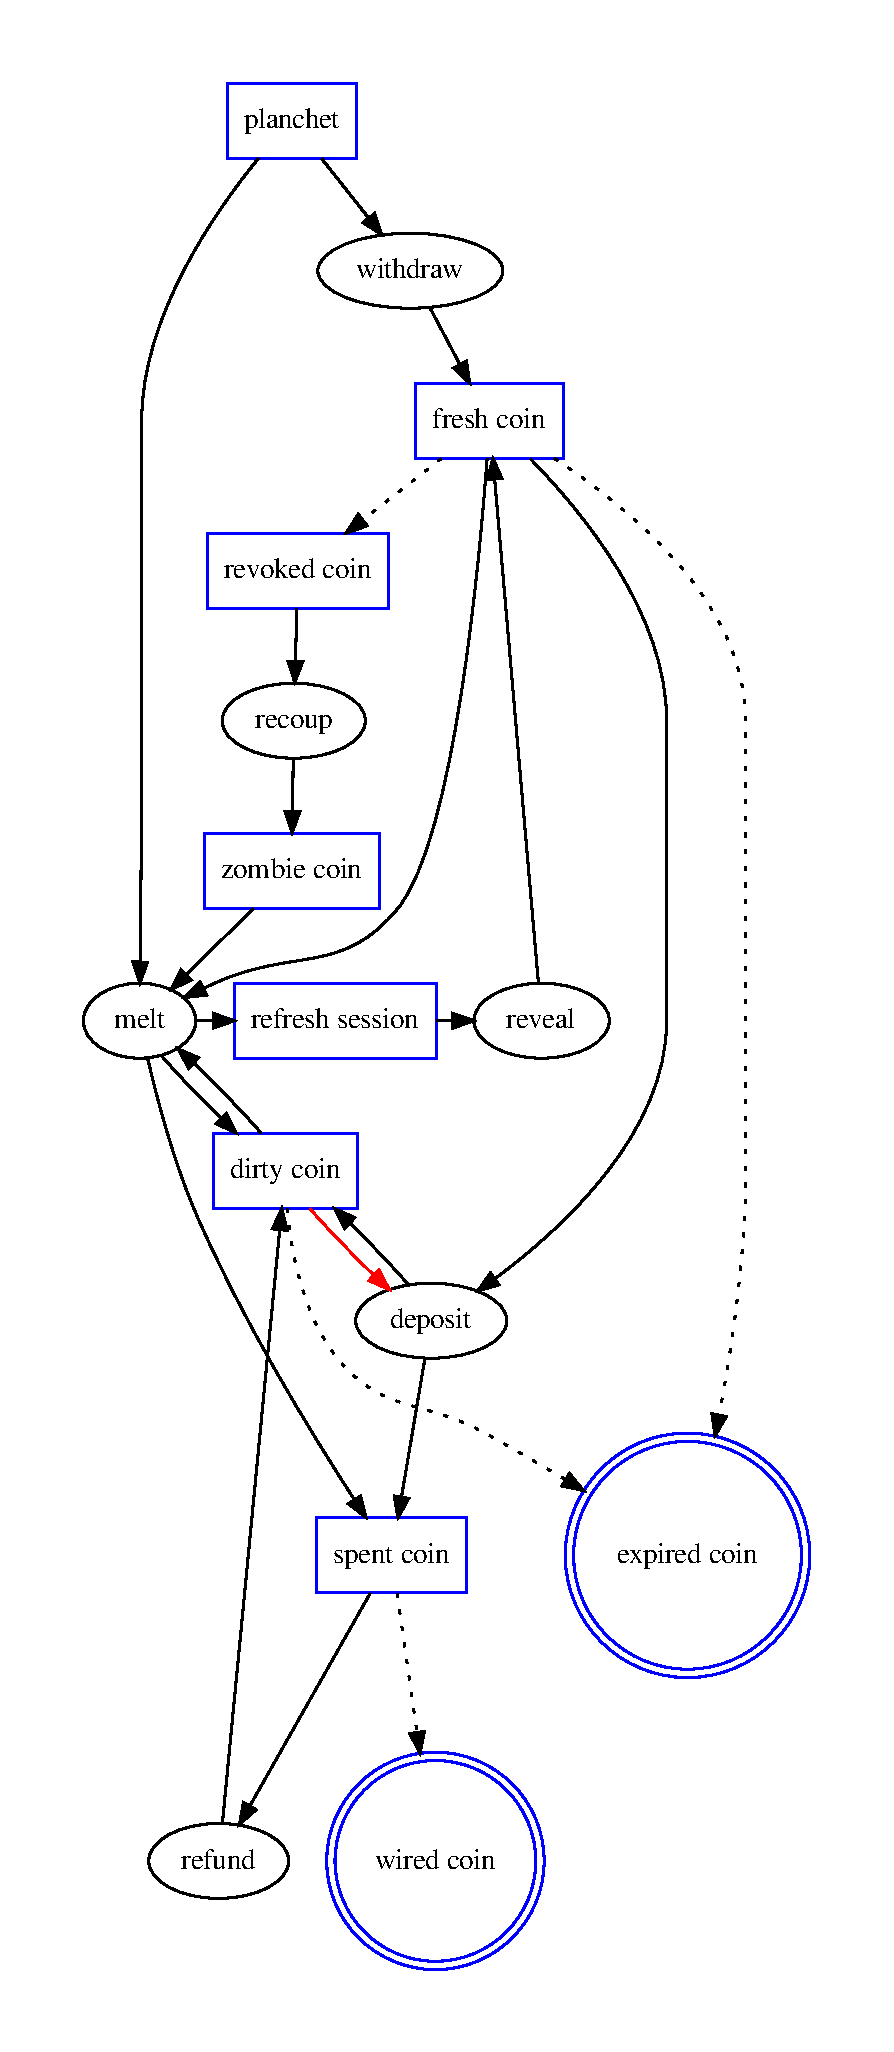
\includegraphics[scale=0.75]{taler/coin.pdf}
  \end{center}
  \caption{State machine of a coin.}
  \label{fig:coin:states}
\end{figure}





\section{Related Work}
% FIXME: Stuff to review/include:
% Blindly Signed Contracts: Anonymous On-Blockchain and Off-Blockchain Bitcoin Transactions
% zcash taxability stuff

\subsection{Anonymous E-Cash}\label{sec:related-work:e-cash}

Chaum's seminal paper \cite{chaum1983blind} introduced blind signatures and
demonstrated how to use them for online e-cash.  Later work
\cite{chaum1989efficient,chaum1990untraceable} introduced offline spending, where additional
information is encoded into coins in such a way that double spending reveals
the culprit's identity.

Okamoto \cite{okamoto1995efficient} introduced the first efficient offline
e-cash scheme with divisibility, a feature that allows a single coin to be
spent in parts.  With Okamoto's protocol, different spending operations that
used parts of the same coin were linkable.  An unlinkable version of
divisible e-cash was first presented by Canard~\cite{canard2007divisible}.

Camenisch's compact e-cash \cite{camenisch2005compact} allows wallets with $2^\ell$ coins to be stored
and withdrawn with storage, computation and computational costs in $\mathcal{O}(\ell)$.
Each coin in the wallet, however, still needs to be spent separately.

The protocol that can currently be considered the state-of-the-art for efficient
offline e-cash was introduced by Pointcheval et al. \cite{pointcheval2017cut}.
It allows constant-time withdrawal of a divisible coin, and constant-time
spending of a continuous ``chunk'' of a coin.  While the pre-determined number
of divisions of a coin is independent from the storage, bandwidth and
computational complexity of the wallet, the exchange needs to check for
double-spending at the finest granularity.  Thus, highly divisible coins incur
large storage and computational costs for the exchange.

An e-cash system with multiple denominations with different financial values
was proposed by Canard and Gouget~\cite{canard2006handy} in the context of a divisible
coupon system.

One of the earliest mentions of an explicit change protocol can be found in
\cite{brickell1995trustee}.  Ian Goldberg's HINDE system is another design that
allows the merchant to provide change, but the mechanism could be abused to
hide income from taxation.\footnote{Description based on personal
communication. HINDE was never published, but supposedly publicly discussed at
Financial Crypto '98.}  Another online e-cash protocol with change was proposed
by Tracz \cite{tracz2001fair}.  The use of an anonymous change protocol (called
a ``refund'' in their context) for fractional payments has also been suggested
for a public transit fees payment system \cite{rupp2013p4r}.  Change protocols
for offline e-cash were recently proposed \cite{batten2018offline}.  To the
best of our knowledge, no change protocol with protections against tax evasion
has been proposed so far, and all change protocols suggested so far can be
(ab)used to make a payment into another wallet.

Transferable e-cash allows the transfer of funds between customers without
using the exchange as in intermediary \cite{fuchsbauer2009transferable}.

Chaum also proposed wallets with observers \cite{chaum1992wallet} as a
mechanism against double spending.  The observer is a tamper-proof hardware
security module that prevents double-spending, while at the same time being
unable to de-anonymize the user.

Various works propose mechanisms to selectively de-anonymize customers or
transactions that are suspected of criminal activities
\cite{stadler1995fair,davida1997anonymity}.  Another approach suspends
customers that were involved in a particular transaction, while keeping the
customer anonymous \cite{au2011electronic}.

One of the first formal treatments of the provable security of e-cash was given
in \cite{damgaard2007proof}.  The first complete security definition for blind
signatures was given by Pointcheval \cite{pointcheval1996provably} and applied
to RSA signatures later \cite{pointcheval2000security}.  While the security
proof of RSA signatures requires the random oracle model, many blind signature
schemes are provably secure in the standard model
\cite{izabachene2013divisible,pointcheval2017cut}.  While most literature
provides only ``human-verified'' security arguments, the security of a simple
e-cash scheme has been successfully modeled in
ProVerif~\cite{dreier2015formal}, albeit only in the symbolic model.

\subsubsection{Implementations}
DigiCash was the first commercial implementation of Chaum's e-cash.  It
ultimately failed to be widely adopted, and the company filed for bankruptcy in
1998.  Some details of the implementation are available
\cite{schoenmakers1997security}.  In addition to Chaum's infamously paranoid
management style \cite{next1999digicash}, reasons for DigiCash's failure could
have been the following:

\begin{itemize}
 \item DigiCash did not allow account-less operations.  To use DigiCash,
   customers had to sign up with a bank that natively supports DigiCash.
 \item DigiCash did not support change or partial spending, negating a lot of
   the convenience and security of e-cash by requiring frequent withdrawals
    from the customer's bank account.
 \item The technology used by DigiCash was protected by patents,
   which stifled innovation from competitors.
 \item Chaum's published design does not clearly limit the financial damage an
   exchange might suffer from the disclosure of its private online signing key.
\end{itemize}

To our knowledge, the only publicly available effort to implement anonymous
e-cash is Opencoin~\cite{dent2008extensions}.  However, Opencoin is neither
actively developed nor used, and it is not clear to what degree the
implementation is even complete.  Only a partial description of the Opencoin
protocol is available to date.


\subsubsection{Representing Denominations}\label{design:related-different-denominations}

For GNU Taler, we chose to represent denominations of different values by a
different public key for every denomination, together with a mapping from
public key to financial value and auxiliary information about fees and
expiration dates.  This approach has the advantage that coins of higher denominations
can be signed by denominations with a larger key size.

Schoenmakers~\cite{schoenmakers1997security} proposes an optimized
implementation of multiple denomination that specifically works with RSA keys,
which encodes the denomination in the public exponent $e$ of the RSA public
key, while the modulus $N$ stays the same for all denominations.  An advantage
of this scheme is the reduced size of the public keys for a set of
denominations.  As this encoding is specific to RSA, it would be difficult for
future versions of this protocol to switch to different blind signature
primitives.  More importantly, factoring $N$ would lead to a compromise of all
denominations instead of just one.

Partially blind signatures can be used to represent multiple denominations
by blindly signing the coin's serial number and including the financial value of the coin
in the common information seen by both the signer and signee \cite{abe2000provably}.

The compact e-cash scheme of Märtens~\cite{maertens2015practical} allows
constant-time withdrawal of wallets with an arbitrary number of coins, as long
as the number of coins is smaller than some system parameter.  This approach
effectively dispenses with the need to have different denominations.


\subsubsection{Comparison}

\newcommand\YES{\ding{51}} % {\checkmark}
\newcommand\NO{\ding{55}}

\newcommand*\rot{\multicolumn{1}{R{45}{1em}}}% no optional argument here, please!
%\newcommand*\rot{}% no optional argument here, please!


\newcolumntype{H}{>{\setbox0=\hbox\bgroup}c<{\egroup}@{}}

\newcolumntype{R}[2]{%
    >{\adjustbox{angle=#1,lap=\width-(#2)}\bgroup}%
    l%
    <{\egroup}%
}

{\footnotesize
\begin{tabular}{r|ccccccccccc}
&
\rot{Year} &
\rot{Implementation} &
%
\rot{Offline spending} &
\rot{Safe aborts/backups} &
\rot{Key expiration} &
%
\rot{Income transparency} &
%
% \rot{Withdrawal cost} & \rot{Deposit cost} &
\rot{No trusted setup} &
\rot{Storage for wallet} &
\rot{Storage for exchange} &
%
\rot{Change/Divisibility} &
\rot{Receipts \& Refunds}
\\ \hline
Chaum \cite{chaum1983blind}
& 1983 & P
&  \NO & \NO & ?
& ?
% &  $\log n$ & $\log n$
&  \YES & $\log n$ & $\log n$
&  \NO & \NO
\\
DigiCash \cite{schoenmakers1997security}
& 1990 & P
&  \NO & \YES & \YES
& \NO
&  \YES & $\log n$ & $\log n$
&  \NO & \NO
\\
Offline Chaum \cite{chaum1990untraceable}
& 1990 & ?
&  \YES & \NO & ?
& ?
&  \YES & $\log n$ & $\log n$
&  \NO & \NO
\\
Tracz \cite{tracz2001fair} % HINDE
& 2001 & E
&  \NO & \YES & ?
& \NO
&  \YES & $\log n$ & $\log n$
&  Onl. & \NO
\\
Compact \cite{camenisch2005compact}
& 2005 & \NO
&  \YES & \NO & ?
&  ?
&  \YES & $\log n$ & $n$ % We're guessing trustless anonymity because not trusted setup
& Off. & \NO
% \\
% Martens \cite{maertens2015}
% & 2015 & \NO
% &  \NO & \NO & %?
% &  \NO &  S & \NO
% % &  $\log n$ & $\log n$
% &  \YES & \NO & W % We're guessing trustless anonymity because not trusted setup
% & OFF & \NO
\\
Divisible \cite{pointcheval2017cut}
& 2017 & \NO
&  \YES & \NO & ?
& ?
&  \NO & $1$ & $n$
& Off. & \NO
\\
GNU Taler
& 2017 & FS
&  \NO & \YES & \YES
&  \YES
% &  $\log n$ & $\log n$
&  \YES & $\log n$ & $\log n$
&  Onl. & \YES
\\ \hline
\end{tabular}
}


\begin{itemize}
  \item \textbf{Implementation.}
    Is there an implementation?  Is it proprietary (P), experimental (E), or free software (FS).
  \item \textbf{Offline Spending}
    Can spending happen offline with delayed detection of double spenders, or
    is double spending detected immediately during spending?
  \item \textbf{Safe abort/backup.}
    Is anonymity preserved in the presence of interrupted operations
    or restoration from backups?  Inherently conflicts with offline double
    spending detection in all approaches that we are aware of.
    We specify ``\YES'' also for schemes that do not explicitly treat aborts/backup,
    but would allow a safe implementation when aborts/backups happen.
  \item \textbf{Key expiration.}
    We specify ``?'' for schemes that do not explicitly discuss key expiration,
    but do not fundamentally conflict with the concept.
  \item \textbf{Income transparency.}
    We specify ``\YES'' if income transparency is supported, ``\NO'' if some feature of
    the scheme conflicts with income transparency and ``?'' if it might be possible
    to add income transparency.
  \item \textbf{No trusted setup.}
    In a trusted setup, some parameters and cryptographic keys are generated
    by a trusted third party.  A compromise of the trusted setup phase can mean loss
    of anonymity.
  \item \textbf{Storage for wallet/exchange.}
    The expected storage for coins adding up to arbitrary value $n$ is specified,
    with some reasonable upper bound for $n$.
  \item \textbf{Change/Divisibility.}
    Can customers pay without possessing exact change?  If so, is it handled
    by giving change online (Onl.) or by divisible coins that support offline
    operation (Off.)?
  \item \textbf{Receipts \& Refunds.}
    The customer either can prove that they payed for
    a contract, or they can get their (unlinkable) money back.
    Also merchants can issue refunds for completed transactions.
    These operations must not introduce linkability or otherwise
    compromise the customer's anonymity.
\end{itemize}


\subsection{Blockchains}
The term ``blockchain'' refers to a wide variety of protocols and systems concerned with
maintaining a ledger---typically involving financial transactions---in a
distributed and decentralized manner.\footnote{Even though there is a centralization tendency
from various sources in practice \cite{walch2019deconstructing}.}

The first and most prominent system that would be categorized as a
``blockchain'' today\footnote{The paper that introduces Bitcoin does not
mention the term ``blockchain''} is Bitcoin \cite{nakamoto2008bitcoin},
published by an individual or group under the alias ``Satoshi Nakamoto''.  The
document timestamping service described in \cite{haber1990time} could be seen
as an even earlier blockchain that predates Bitcoin by about 13
years and is still in use today.

As the name implies, blockchains are made up of a chain of blocks, each block
containing updates to the ledger and the hash code of its predecessor block. The
chain terminates in a ``genesis block'' that determines the initial state of
the ledger.

Some of the most important decisions for the design of blockchains are the following:
\begin{itemize}
  \item The \emph{consensus mechanism}, which determines how the participants
    agree on the current state of the ledger.

    In the simplest possible blockchain, a trusted authority would validate
    transactions and publish new blocks as the head of the chain.  In order to
    increase fault tolerance, multiple trusted authorities can use Byzantine
    consensus to agree on transactions.  With classical Byzantine consensus
    protocols, this makes the system robust with a malicious minority of up to
    $1/3$ of nodes.  While fast and appropriate for some applications,
    classical Byzantine consensus only works with a known set of participants
    and does not scale well to many nodes.

    Bitcoin instead uses Proof-of-Work (PoW) consensus, where the head of the
    chain that determines the current ledger state is chosen as the block that
    provably took the most ``work'' to construct, including the accumulated
    work of ancestor blocks.  The work consists of finding a hash preimage $n
    \Vert c$, where $c$ are the contents of the block and $n$ is a nonce, such
    that the hash $H(n \Vert c)$ ends with a certain number of zeroes (as
    determined by the difficulty derived from previous blocks).  Under the
    random oracle, the only way to find such a nonce is by trial-and-error.
    This nonce proves to a verifier that the creator of the block spent
    computational resources to construct it, and the correctness is easily
    verified by computing $H(n \Vert c)$.  The creator of a block is rewarded
    with a mining reward and transaction fees for transactions within the
    block.

    PoW consensus is not final:  an adversary with enough computational power
    can create an alternate chain branching off an earlier block.  Once this
    alternative, longer chain is published, the state represented by the
    earlier branch is discarded.  This creates a potential for financial fraud,
    where an earlier transaction is reversed by publishing an alternate history
    that does not contain it.  While it was originally believed that PoW
    consensus process is resistant against attackers that have less than a
    $51\%$ majority of computational power, closer analysis has shown that a
    $21\%$ majority sufficies \cite{eyal2018majority}.

    A major advantage of PoW consensus is that the participants need not be
    known beforehand, and that Sybil attacks are impossible since consensus
    decisions are only dependent on the available computational power, and not
    on the number of participants.

    In practice, PoW consensus is rather slow:  Bitcoin can currently support
    3-7 transactions per second on a global scale.  Some efforts have been made
    to improve Bitcoin's efficiency \cite{eyal2016bitcoin,vukolic2015quest},
    but overall PoW consensus needs to balance speed against security.

    Proof-of-Stake (PoS) is a different type of consensus protocol for
    blockchains, which intends to securely reach consensus without depleting
    scarce resources such as energy for computation
    \cite{bentov2016cryptocurrencies,kwon2014tendermint}.  Blocks are created
    by randomly selected validators, which obtain a reward for serving as a
    validator.  To avoid Sybil attacks and create economic incentives for good
    behavior, the probability to get selected as a validator is proportional to
    one's wealth on the respective blockchain.  Realizing PoS has some
    practical challenges with respect to economic incentives: As blocks do not
    take work to create, validators can potentially benefit from creating
    forks, instead of validating on just one chain.

    Algorand \cite{gilad2017algorand} avoids some of the problems with PoW
    consensus by combining some of the ideas of PoW with classical Byzantine
    consensus protocols.  Their proposed system does not have any incentives
    for validators.

    Avalance \cite{rocket2018snowflake} has been proposed as a scalable
    Byzantine Consensus algorithm for use with blockchains.  It is based on a
    gossip protocol and is only shown to work in the synchronous model.

  \item Membership and visibility.  Blockchains such as Bitcoin or Ethereum with
    public membership and public visibility are called \emph{permissionless blockchains}.
    Opposed to that, \emph{permissioned} blockchains have been proposed for usage in
    banking, health and asset tracking applications \cite{androulaki2018hyperledger}.

  \item Monetary policy and wealth accumulation.
    Blockchains that are used as cryptocurrencies come with their own monetary
    policy.  In the case of Bitcoin, the currency supply is limited, and due to
    difficulty increase in mining the currency is deflationary.  Other
    cryptocurrencies such as duniter\footnote{See
    \url{https://duniter.org/}.} have been proposed with built-in rules for
    inflation, and a basic income mechanism for participants.

  \item Expressivity of transactions.  Transactions in Bitcoin are small programs
    in a stack-based programming language that are guaranteed to terminate.
    Ethereum \cite{wood2014ethereum} takes this idea further and allows smart contracts with
    Turing-complete computation and access to external oracles.

  \item Governance.  Blockchain governance \cite{reijers2016governance,levy2017book} is a
    topic that received relatively little attention so far.  As blockchains
    interact with existing legal and social systems across national borders,
    different sources of ``truth'' must be reconciled.

    Furthermore, consensus is not just internal to the operation of
    blockchains, but also external in the development of the technology.
    Currently small groups of developers create the rules for the operation of
    blockchains, and likewise have the power to change them.  There is
    currently very little research on social and technological processes to
    find a ``meta-consensus'' on the rules that govern such systems, and how
    these rules can be adapted and changed in a consensus process.

  \item Anonymity and Zero-Knowledge Proofs.  Bitcoin transactions are only
    pseudoymous, the full transaction history is publicly available and leads
    to reduced anonymity in practice \cite{reid2013analysis}.  Tumblers
    \cite{bonneau2014mixcoin,heilman2017tumblebit} are an approach to increase
    the anonymity in Bitcoin-style cryptocurrencies by creating additional
    transactions to cover up the real owner and sources of funds.  While newer tumblers
    such as TumbleBit \cite{heilman2017tumblebit} provide rather strong security guarantees,
    mixing incurs transaction costs.

    Some cryptocurrencies have direct support for anonymous transactions
    \cite{sun2017ringct}.  ZeroCash \cite{bensasson2014zerocash} uses
    zero-knowledge proofs to hide the sender, receiver and amount of a
    transaction.  While ZeroCash currently relies on a trusted setup for
    unforgeability of its currency, more recent proposals dispense with that
    requirement \cite{ben2018scalable,wahby2018doubly}.  As the anonymity
    provided by ZeroCash facilitates tax evasion and use in other crimes, an
    additional, optional layer for privacy-preserving policy for taxation,
    spending limits and identity escrow has been proposed
    \cite{garman2016accountable}.
\end{itemize}

Practical guidance on what kind of blockchain is appropriate for an
application, and if a blockchain is required in the first place, can be found
in \cite{wust2017you}.


\subsection{Approaches to Micropayments}
Micropayments refer to payments of very small value. Microtransactions would
not be feasible in traditional payment systems due to high transaction costs,
which might even exceed that value that is to be transferred.

\subsubsection{Peppercoin}

Peppercoin~\cite{rivest2004peppercoin} is a microdonation protocol.
The main idea of the protocol is to reduce transaction costs by
minimizing the number of transactions that are processed directly by
the exchange.  Instead of always paying, the customer ``gambles'' with the
merchant for each microdonation.  Only if the merchant wins, the
microdonation is upgraded to a macropayment to be deposited at the
exchange.  Peppercoin does not provide customer-anonymity.  The proposed
statistical method by which exchanges detect fraudulent cooperation between
customers and merchants at the expense of the exchange not only creates
legal risks for the exchange, but would also require that the exchange learns
about microdonations where the merchant did not get upgraded to a
macropayment.  It is therefore unclear how Peppercoin would actually
reduce the computational burden on the exchange.

\subsubsection{Tick Payments}
% FIXME:  also works off-line
Tick payments were proposed by Pedersen \cite{pedersen1996electronic} as a
general technique to amortize the cost for small, recurring payments to the
same payee.  The payer first makes an up-front deposit as one larger payment
that involves the payment processor.  To make a micropayment, the payer sends a
message to the payee that authorizes the payee to claim a fraction of this
deposit.  Each further micropayment simply increases the fraction of the
deposit that can be claimed, and only requires communication between payer and
payee.  The payee only needs to show the last message received from the payer
to the payment processor in order to receive the accumulated amounts received
through tick payments.

\subsubsection{Payment Channels and Lightning Network}
The Lightning Network \cite{poon2016bitcoin} is a proposed payment system that
is meant to run on top of Bitcoin and enable faster, cheaper
(micro-)transactions.  It is based on establishing \emph{payment channels}
between Bitcoin nodes.  A payment channel is essentially a tick payment where
the deposit and settlement happens on a blockchain.  The goal of the
Lightning network is to route a payment between two arbitrary nodes by finding a
path that connects the two routes through payment channels.  The protocol is
designed in such a way that a node on the path between the initial sender and
final receiver can only receive a payment on a payment channel if it correctly
forwards it to the next node.

Experimental deployments of the Lightning network recently suffered heavily
from denial-of-service attacks. % FIXME: citation needed!

BOLT \cite{green2016bolt} is an anonymous payment channel for ZeroCash, and is
intended to be used as a building block for a second-layer payment protocol
like the Lightning Network.

\subsubsection{Side-chains}
% FIXME:  what about polkadot?
Side-chains are an alternative approach to improve the scalability of
blockchains, intended to be useful in conjunction with arbitrary smart
contracts.  The approach currently developed by the Ethereum project is
described in the Plasma white paper \cite{poon2017plasma}.  Side-chains are
separate blockchains, possibly with different rules and even consensus
protocols than the main chain.  Side-chains operate in parallel to the main
Ethereum chain, and regularly publish ``pointers'' to the current head of the
sidechain on the main chain.  Funds can be moved from the main chain to the
side-chain, and subsequently be moved off the side-chain by performing an
``exit'', during which the main chain verifies claims to funds on the
side-chain according to the side-chain's rules.

At the time of writing, Plasma is not yet implemented.  Potential problems with
Plasma include the high costs of exits, lack of access to data needed to verify
exit claims, and associated potential for denial-of-service attacks.


%\subsection{Other Payment Systems}

%\subsubsection{Credit Card Payments}

\subsection{Walled Garden Payment Systems}

Walled garden payment systems offer ease of use by processing payments using a
trusted payment service provider. Here, the customer authenticates to the
trusted service, and instructs the payment provider to execute a transaction on
their behalf.  In these payment systems, the provider basically acts like a
bank with accounts carrying balances for the various users.  In contrast to
traditional banking systems, both customers and merchants are forced to have an
account with the same provider.  Each user must take the effort to establish
his identity with a service provider to create an account.  Merchants and
customers obtain the best interoperability in return for their account creation
efforts if they start with the biggest providers.  As a result, there are a few
dominating walled garden providers, with AliPay, ApplePay, GooglePay,
SamsungPay and PayPal being the current oligopoly.
%In this paper, we
%will use PayPal as a representative example for our discussion of these payment
%systems.

As with card payment systems, these oligopolies are politically
dangerous~\cite{crinkey2011rundle}, and the lack of competition
can result in excessive profit taking that may require political
solutions~\cite{guardian2015cap} to the resulting market
  failure.  The use of non-standard proprietary interfaces to
the payment processing service of these providers serves to reinforce
the customer lock-in.

%TODO: discuss popularity/abundance of digital wallets in other countries (India!)
%and different requirements (connectivity)

%\subsubsection{Ripple}

\subsection{Web Integration}

Finally, we will discuss software solutions to web payments.  We
consider other types of payments, including general payments and in
particular hardware solutions as out of scope for this thesis.

\subsubsection{Web Payments API}
The Web Payments API\footnote{See \url{https://www.w3.org/TR/payment-request/}}
is a JavaScript API offered by browsers, and currently still under development.
It allows merchant to offer a uniform checkout experience across different
payment systems.  Unlike GNU Taler, the Web Payments API is only concerned with
aspects of the checkout process, such as display of a payment request,
selection of a shipping address and selection of a payment method.

Currently only basic-card is supported across popular browsers.

The Payment Handler API\footnote{See
\url{https://www.w3.org/TR/payment-handler/}} supports the registration of
user-defined payment method handlers.  Unfortunately the only way to add
payment method handlers is via an HTTPS URL.  This leaks all information to the
payment service provider and precludes the implementation of privacy-preserving
payment system handlers.

In order to integrate Taler as a payment method, browsers would need to either
offer Taler as a native, built-in payment method or allow an extension to
register web payment handlers.


The Web Payments Working Group discontinued work on a HTTP-based API for
machine-to-machine payments.\footnote{See
\url{https://www.w3.org/TR/webpayments-http-api/}.}

\subsubsection{Payment Pointers}
Payment pointers are a proposed standard syntax for accounts that are able to
receive payments.  Unlike \texttt{payto://} URIs ( discussed in
Section~\ref{implementation:wire-method-identifiers}), payment pointers do not
follow the generic URI syntax and only specify a \emph{pointer} to the
receiver's bank account in form of a HTTPS URI.  Payment pointers do not
specify any mechanism for the payment, but instead direct the user's browser to
a website to carry out the payment.

\subsubsection{3-D Secure}
3-D Secure is a complex and widely deployed protocol that is intended to add an
additional security layer on top of credit and debit card transactions.

The 3-D Secure protocol requires the use of inline frames on the HTML page of
the merchant for extended verification/authentication of the user.  This makes
it hard or sometimes -- such as when using a mobile browser -- even impossible
to tell whether the inline frame is legitimate or an attempt to steal
information from the user.

Traditionally, merchants bear most of the financial risk, and a key
``feature'' of the 3DS process compared to traditional card payments
is to shift dispute {\em liability} to the issuer of the card---who
may then try to shift it to the customer \cite[\S2.4]{3DSsucks}.
%
% online vs offline vs swipe vs chip vs NFC ???
% extended verification
%
Even in cases where the issuer or the merchant remain legally first in
line for liabilities, there are still risks customers incur from the
card dispute procedures, such as neither them nor the payment
processor noticing fraudulent transactions, or them noticing
fraudulent transactions past the {\em deadline} until which their bank
would reimburse them.  The customer also typically only has a
merchant-generated comment and the amount paid in their credit card
statement as a proof for the transaction.  Thus, the use of credit
cards online does not generate any cryptographically {\em verifiable}
electronic receipts for the customer, which theoretically enables
malicious merchants to later change the terms of the contract.

Beyond these primary issues, customers face secondary risks of
identity theft from the personal details exposed by the authentication
procedures. In this case, even if the financial damages are ultimately
covered by the bank, the customer always has to deal with the procedure
of {\em notifying} the bank in the first place.  As a result,
customers must remain wary about using their cards, which limits their
online shopping~\cite[p. 50]{ibi2014}.

\subsubsection{Other Proprietary Payment APIs}
The Electronic Payment Standard URI scheme \texttt{epspayment:} is a
proprietary/unregistered URI scheme used by predominantly Austrian banks and
merchants to trigger payments from within websites on mobile devices.
Merchants can register an invoice with a central server.  The user's banking
app is associated with the \texttt{epspayment} URI scheme and will open to
settle the invoice.  It lies conceptually between \texttt{payto://} and
\texttt{taler:pay} (see Section~\ref{sec:loose-browser-integration}).  A
technical problem of \texttt{epspayment} is that when a user has multiple bank
accounts at different banks that support \texttt{epspayment}, some platforms
decide non-deterministically and without asking the user which application to
launch.  Thus, a user with two banking applications on their phone can often not
chose which bank account is used for the payment.  If \texttt{payto} were
widely supported, the problem of registering/choosing bank accounts for payment
methods could be centrally addressed by the browser / operating system.

PayPal is a very popular, completely proprietary payment system provider.  Its offer-based
API is similar in the level of abstraction to Taler's reference merchant backend API.

LaterPay is a proprietary payment system for online content as well as
donations.  It offers similar functionality to session-bound payments in Taler.
LaterPay does not provide any anonymity.


% FIXME: mention these
% Stripe
% paydirekt
% mention this somewhere: https://www.focus.de/finanzen/banken/paydirekt-so-reagieren-kunden-auf-die-sparkassen-plaene_id_7511393.html
% but not in this section.  good argument for anonymity

\chapter{Security of Income-Transparent Anonymous E-Cash}\label{chapter:security}

\def\Z{\mathbb{Z}}

\def\mathperiod{.}
\def\mathcomma{,}

\newcommand*\ST[5]%
{\left#1\,#4\vphantom{#5} \;\right#2 \left. #5 \vphantom{#4}\,\right#3}

% uniform random selection from set
\newcommand{\randsel}[0]{\ensuremath{\xleftarrow{\text{\$}}}}

\newcommand{\Exp}[1]{\ensuremath{E\left[#1\right]}}

% oracles
\newcommand{\ora}[1]{\ensuremath{\mathcal{O}\mathsf{#1}}}
% oracle set
\newcommand{\oraSet}[1]{\ensuremath{\mathcal{O}\textsc{#1}}}
% algorithm
\newcommand{\algo}[1]{\ensuremath{\mathsf{#1}}}
% party
\newcommand{\prt}[1]{\ensuremath{\mathcal{#1}}}
% long-form variable
\let\V\relax % clashes with siunitx volt
\newcommand{\V}[1]{\ensuremath{\mathsf{#1}}}

% probability with square brackets of the right size
\newcommand{\Prb}[1]{\ensuremath{\Pr\left [#1 \right ]}}

\newcommand{\mycomment}[1]{~\\ {\small \textcolor{blue}{({#1})}}}

\theoremstyle{definition}
\newtheorem{definition}{Definition}[section]
\theoremstyle{corollary}
\newtheorem{corollary}{Corollary}[section]


%%%%%%%%%
% TODOS
%%%%%%%%
% 
% * our theorems don't really mention the security parameters "in the output",
%   shouldn't we be able to talk about the bounds of the reduction?

We so far discussed Taler's protocols and security properties only informally.
In this chapter, we model a slightly simplified version of the system that we
have implemented (see Chapter~\ref{chapter:implementation}), make our desired
security properties more precise, and prove that our protocol instantiation
satisfies those properties.

\section{Introduction to Provable Security}
Provable security
\cite{goldwasser1982probabilistic,pointcheval2005provable,shoup2004sequences,coron2000exact} is a common
approach for constructing formal arguments that support the security of a cryptographic
protocol with respect to specific security properties and underlying
assumptions on cryptographic primitives.

The adversary we consider is computationally bounded, i.e., the run time is
typically restricted to be polynomial in the security parameters (such as key
length) of the protocol.

Contrary to what the name might suggest, a protocol that is ``provably secure''
is not necessarily secure in practice
\cite{koblitz2007another,damgaard2007proof}.  Instead, provable security
results are typically based on reductions of the form \emph{``if there is an
effective adversary~$\mathcal{A}$ against my protocol $P$, then I can use
$\mathcal{A}$ to construct an effective adversary~$\mathcal{A}'$ against
$Q$''} where $Q$ is a protocol or primitive that is assumed to be secure or a
computational problem that is assumed to be hard.  The practical value of a
security proof depends on various factors:
\begin{itemize}
  \item How well-studied is $Q$? Some branches of cryptography, for example,
    some pairing-based constructions, rely on rather complex and exotic
    underlying problems that are assumed to be hard (but might not be)
    \cite{koblitz2010brave}.
  \item How tight is the reduction of $Q$ to $P$?  A security proof may only
    show that if $P$ can be solved in time $T$, the underlying problem $Q$ can
    be solved (using the hypothetical $\mathcal{A}$) in time, e.g., $f(T) = T^2$.
    In practice, this might mean that for $P$ to be secure, it needs to be deployed
    with a much larger key size or security parameter than $Q$ to be secure.
  \item What other assumptions are used in the reduction?  A common and useful but
    somewhat controversial
    assumption is the Random Oracle Model (ROM) \cite{bellare1993random}, where
    the usage of hash functions in a protocol is replaced with queries to a
    black box (called the Random Oracle), which is effectively a trusted third
    party that returns a truly random value for each input.  Subsequent queries
    to the Random Oracle with the same value return the same result.  While
    many consider ROM a practical assumption
    \cite{koblitz2015random,bellare1993random}, it has been shown that there
    exist carefully constructed protocols that are secure under the ROM, but
    are insecure with any concrete hash function \cite{canetti2004random}.  It
    is an open question whether this result carries over to practical
    protocols, or just certain classes of artificially constructed protocols of
    theoretical interest.
\end{itemize}
Furthermore, a provably secure protocol does not always lend itself easily to a secure
implementation, since side channels and fault injection attacks \cite{hsueh1997fault,lomne2011side} are
usually not modeled. Finally, the security properties stated might
not be sufficient or complete for the application.

For our purposes, we focus on game-based provable security
\cite{bellare2006code,pointcheval2005provable,shoup2004sequences,guo2018introduction}
as opposed to simulation-based provable security \cite{goldwasser1989knowledge,lindell2017simulate},
which is another approach to provable security typically used for
zero-knowledge proofs and secure multiparty computation protocols.

\subsection{Algorithms, Oracles and Games}
In order to analyze the security of a protocol, the protocol and its desired
security properties against an adversary with specific capabilities must first
be modeled formally.  This part is independent of a concrete instantiation of
the protocol; the protocol is only described on a syntactic level.

The possible operations of a protocol (i.e., the protocol syntax) are abstractly
defined as the signatures of \emph{algorithms}.  Later, the protocol will be
instantiated by providing a concrete implementation (formally a program for a
probabilistic Turing machine) of each algorithm. A typical public key signature
scheme, for example, might consist of the following algorithms:
\begin{itemize}
  \item $\algo{KeyGen}(1^\lambda) \mapsto (\V{sk}, \V{pk})$, a probabilistic algorithm
    which on input $1^\lambda$ generates a fresh key pair consisting of secret key $\V{sk}$ of length $\lambda$ and
    and the corresponding public key $\V{pk}$.  Note that $1^\lambda$ is the unary representation of $\lambda$.\footnote{%
    This formality ensures that the size of the input of the Turing machine program implementing the algorithm will
    be as least as big as the security parameter.  Otherwise the run-time complexity cannot be directly expressed
    in relation to the size of the input tape.}
  \item $\algo{Sign}(\V{sk}, m) \mapsto \sigma$, an algorithm
    that signs the bit string $m$ with secret key $\V{sk}$ to output the signature $\sigma$.
  \item $\algo{Verify}(\V{pk}, \sigma, m) \mapsto b$, an algorithm
    that determines whether $\sigma$ is a valid signature on $m$ made with the secret key corresponding to the
    public key $\V{pk}$.  It outputs the flag $b \in \{0, 1\}$ to indicate whether the signature
    was valid (return value $1$) or invalid (return value $0$).
\end{itemize}
The abstract syntax could be instantiated with various concrete signature protocols.

In addition to the computational power given to the adversary, the capabilities
of the adversary are defined via oracles.  The oracles can be thought of as the
API\footnote{In the modern sense of application programming interface (API),
where some system exposes a service with well-defined semantics.} that is given
to the adversary and allows the adversary to interact with the environment it
is running in.  Unlike the algorithms, which the adversary has free access to,
the access to oracles is often restricted, and oracles can keep state that is
not accessible directly to the adversary.  Oracles typically allow the
adversary to access information that it normally would not have direct access
to, or to trigger operations in the environment running the protocol.

Formally, oracles are an extension to the Turing machine that runs the
adversary, which allow the adversary to submit queries to interact with the
environment that is running the protocol.


For a signature scheme, the adversary could be given access to an \ora{Sign}
oracle, which the adversary uses to make the system produce signatures, with
secret keys that the adversary does not have direct access to.  Different
definitions of \ora{Sign} lead to different capabilities of the adversary and
thus to different security properties later on:
\begin{itemize}
  \item If the signing oracle $\ora{Sign}(m)$ is defined to take a message $m$ and return
    a signature $\sigma$ on that message, the adversary gains the power to do chosen message attacks.
  \item If $\ora{Sign}(\cdot)$ was defined to return a pair $(\sigma, m)$ of a signature $\sigma$
    on a random message $m$, the power of the adversary would be reduced to a known message attack.
\end{itemize}

While oracles are used to describe the possible interactions with a system, it
is more convenient to describe complex, multi-round interactions involving
multiple parties as a special form of an algorithm, called an \emph{interactive
protocol}, that takes the identifiers of communicating parties and their
(private) inputs as a parameter, and orchestrates the interaction between them.
The adversary will then have an oracle to start an instance of that particular
interactive protocol and (if desired by the security property being modeled)
the ability to drop, modify or inject messages in the interaction.  The
typically more cumbersome alternative would be to introduce one algorithm and
oracle for every individual interaction step.

Security properties are defined via \emph{games}, which are experiments that
challenge the adversary to act in a way that would break the desired security
property.  Games usually consist multiple phases, starting with the setup phase
where the challenger generates the parameters (such as encryption keys) for the
game.  In the subsequent query/response phase, the adversary is given some of
the parameters (typically including public keys but excluding secrets) from the
setup phase, and runs with access to oracles.  The challenger\footnote{ The
challenger is conceptually the party or environment that runs the
game/experiment.} answers oracle queries during that phase.  After the
adversary's program terminates, the challenger invokes the adversary again with
a challenge.  The adversary must now compute a final response to the
challenger, sometimes with access to oracles.  Depending on the answer, the
challenger decides if the adversary wins the game or not, i.e., the game returns
$0$ if the adversary loses and $1$ if the adversary wins.

A game for the existential unforgeability of signatures could be formulated like this:

\bigskip
\noindent $\mathit{Exp}_{\prt{A}}^{EUF}(1^\lambda)$:
\vspace{-0.5\topsep}
\begin{enumerate}
  \setlength\itemsep{0em}
  \item $(\V{sk}, \V{pk}) \leftarrow \algo{KeyGen}(1^\lambda)$
  \item $(\sigma, m) \leftarrow \prt{A}^{\ora{Sign(\cdot)}}(\V{pk})$

    (Run the adversary with input $\V{pk}$ and access to the $\ora{Sign}$ oracle.)
  \item If the adversary has called $\ora{Sign}(\cdot)$ with $m$ as argument,
    return $0$.
  \item Return $\algo{Verify}(\V{pk}, \sigma, m)$.
\end{enumerate}
Here the adversary is run once, with access to the signing oracle.  Depending
on which definition of $\ora{Sign}$ is chosen, the game models existential
unforgeability under chosen message attack (EUF-CMA) or existential
unforgeability under known message attack (EUF-KMA)

The following modification to the game would model selective unforgeability
(SUF-CMA / SUF-KMA):

\bigskip
\noindent $\mathit{Exp}_{\prt{A}}^{SUF}(1^\lambda)$:
\vspace{-0.5\topsep}
\begin{enumerate}
  \setlength\itemsep{0em}
  \item $m \leftarrow \prt{A}()$
  \item $(\V{sk}, \V{pk}) \leftarrow \algo{KeyGen}(1^\lambda)$
  \item $\sigma \leftarrow \prt{A}^{\ora{Sign(\cdot)}}(\V{pk}, m)$
  \item If the adversary has called $\ora{Sign}(\cdot)$ with $m$ as argument,
    return $0$.
  \item Return $\algo{Verify}(\V{pk}, \sigma, m)$.
\end{enumerate}
Here the adversary has to choose a message to forge a signature for before
knowing the message verification key.

After having defined the game, we can now define a security property based on
the probability of the adversary winning the game: we say that a signature
scheme is secure against existential unforgeability attacks if for every
adversary~\prt{A} (i.e., a polynomial-time probabilistic Turing machine
program), the success probability
\begin{equation*}
  \Prb{\mathit{Exp}_{\prt{A}}^{EUF}(1^\lambda) = 1 }
\end{equation*}
of \prt{A} in the EUF game is \emph{negligible} (i.e., grows less fast with
$\lambda$ than the inverse of any polynomial in $\lambda$).

Note that the EUF and SUF games are related in the following way:  an adversary
against the SUF game can be easily transformed into an adversary against the
EUF game, while the converse does not necessarily hold.

Often security properties are defined in terms of the \emph{advantage} of the
adversary.  The advantage is a measure of how likely the adversary is to win
against the real cryptographic protocol, compared to a perfectly secure version
of the protocol.  For example, let $\mathit{Exp}_{\prt{A}}^{BIT}()$ be a game
where the adversary has to guess the next bit in the output of a pseudo-random number
generator (PRNG).  The idealized functionality would be a real random number generator,
where the adversary's chance of a correct guess is $1/2$.  Thus, the adversary's advantage is
\begin{equation*}
  \left|\Prb{\mathit{Exp}_{\prt{A}}^{BIT}()} - 1/2\right|.
\end{equation*}
Note that the definition of advantage depends on the game.  The above
definition, for example, would not work if the adversary had a way to
``voluntarily'' lose the game by querying an oracle in a forbidden way


\subsection{Assumptions, Reductions and Game Hopping}
The goal of a security proof is to transform an attacker against
the protocol under consideration into an attacker against the security
of an underlying assumption.  Typical examples for common assumptions might be:
\begin{itemize}
  \item the difficulty of the decisional/computational Diffie--Hellman problem (nicely described by~\cite{boneh1998decision})
  \item existential unforgeability under chosen message attack (EUF-CMA) of a signature scheme \cite{goldwasser1988digital}
  \item indistinguishability against chosen-plaintext attacks (IND-CPA) of a symmetric
    encryption algorithm \cite{bellare1998relations}
\end{itemize}

To construct a reduction from an adversary \prt{A} against $P$ to an adversary
against $Q$, it is necessary to specify a program $R$ that both interacts as an
adversary with the challenger for $Q$, but at the same time acts as a
challenger for the adversary against $P$.  Most importantly, $R$ can chose how
to respond to oracle queries from the adversary, as long as $R$ faithfully
simulates a challenger for $P$.  The reduction must be efficient, i.e., $R$ must
still be a polynomial-time algorithm.

A well-known example for a non-trivial reduction proof is the security proof of
FDH-RSA signatures \cite{coron2000exact}.
% FIXME:  I think there's better reference, pointcheval maybe?

In practice, reduction proofs are often complex and hard to verify.
Game hopping has become a popular technique to manage the complexity of
security proofs.  The idea behind game hopping proofs is to make a sequence of
small modifications starting from initial game, until you arrive at a game
where the success probability for the adversary becomes obvious, for example,
because the winning state for the adversary becomes unreachable in the code
that defines the final game, or because all values the adversary can observe to
make a decision are drawn from a truly random and uniform distribution.  Each
hop modifies the game in a way such that the success probability of game
$\mathbb{G}_n$ and game $\mathbb{G}_{n+1}$ is negligibly close.

Useful techniques for hops are, for example:
\begin{itemize}
  \item Bridging hops, where the game is syntactically changed but remains
    semantically equivalent, i.e., $\Prb{\mathbb{G}_n = 1} = \Prb{\mathbb{G}_n = 1}$.
  \item Indistinguishability hops, where some distribution is changed in a way that
    an adversary that could distinguish between two adjacent games could be turned
    into an adversary that distinguishes the two distributions.  If the success probability
    to distinguish between those two distributions is $\epsilon$, then
    $\left|\Prb{\mathbb{G}_n = 1} - \Prb{\mathbb{G}_n = 1}\right| \le \epsilon$
  \item Hops based on small failure events.  Here adjacent games proceed
    identically, until in one of the games a detectable failure event $F$ (such
    as an adversary visibly forging a signature) occurs.  Both games most proceed
    the same if $F$ does not occur.  Then it is easy to show \cite{shoup2004sequences}
    that $\left|\Prb{\mathbb{G}_n = 1} - \Prb{\mathbb{G}_n = 1}\right| \le \Prb{F}$
\end{itemize}

A tutorial introduction to game hopping is given by Shoup \cite{shoup2004sequences}, while a more formal
treatment with a focus on ``games as code'' can be found in \cite{bellare2006code}.  A
version of the FDH-RSA security proof based on game hopping was generated with an
automated theorem prover by Blanchet and Pointcheval \cite{blanchet2006automated}.

% restore-from-backup

% TODO:
% - note about double spending vs overspending

\subsection{Notation}
We prefix public and secret keys with $\V{pk}$ and $\V{sk}$, and write $x
\randsel S$ to randomly select an element $x$ from the set $S$ with uniform
probability.

\section{Model and Syntax for Taler}

We consider a payment system with a single, static exchange and multiple,
dynamically created customers and merchants.  The subset of the full Taler
protocol that we model includes withdrawing digital coins, spending them with
merchants and subsequently depositing them at the exchange, as well as
obtaining unlinkable change for partially spent coins with an online
``refresh'' protocol.

The exchange offers digital coins in multiple denominations, and every
denomination has an associated financial value; this mapping is not chosen by
the adversary but is a system parameter.  We mostly ignore the denomination
values here, including their impact on anonymity, in keeping with existing
literature \cite{camenisch2007endorsed,pointcheval2017cut}.  For anonymity, we
believe this amounts to assuming that all customers have similar financial
behavior.  We note logarithmic storage, computation and bandwidth demands
denominations distributed by powers of a fixed constant, like two.

We do not model fees taken by the exchange.  Reserves\footnote{%
  ``Reserve'' is Taler's terminology for funds submitted to the exchange that
  can be converted to digital coins.
}
are also omitted.
Instead of maintaining a reserve balance, withdrawals of different
denominations are tracked, effectively assuming every customer has unlimited funds.

Coins can be partially spent by specifying a fraction $0 < f \le 1$ of the
total value associated with the coin's denomination.  Unlinkable change below
the smallest denomination cannot be given.  In
practice the unspendable, residual value should be seen as an additional fee
charged by the exchange.

Spending multiple coins is modeled non-atomically: to spend (fractions
of) multiple coins, they must be spent one-by-one.  The individual
spend/deposit operations are correlated by a unique identifier for the
transaction.  In practice, this identifier is the hash $\V{transactionId} =
H(\V{contractTerms})$ of the contract terms\footnote{The contract terms
are a digital representation of an individual offer for a certain product or service the merchant sells
for a certain price.}.  Contract terms include a nonce to make them
unique, that merchant and customer agreed upon.  Note that this transaction
identifier and the correlation between multiple spend operations for one
payment need not be disclosed to the exchange (it might, however, be necessary
to reveal during a detailed tax audit of the merchant):  When spending the $i$-th coin
for the transaction with the identifier $\V{transactionId}$, messages to the
exchange would only contain $H(i \Vert \V{transactionId})$.  This is preferable
for merchants that might not want to disclose to the exchange the individual
prices of products they sell to customers, but only the total transaction
volume over time.  For simplicity, we do not include this extra feature in our
model.

Our system model tracks the total amount ($\equiv$ financial value) of coins
withdrawn by each customer.
Customers are identified by their public key $\V{pkCustomer}$.  Every
customer's wallet keeps track of the following data:
\begin{itemize}
  \item $\V{wallet}[\V{pkCustomer}]$ contains sets of the customer's coin records,
   which individually consist of the coin key pair, denomination and exchange's signature.
  \item $\V{acceptedContracts}[\V{pkCustomer}]$ contains the sets of
    transaction identifiers accepted by the customer during spending
    operations, together with coins spent for it and their contributions $0 < f
    \le 1$.
  \item $\V{withdrawIds}[\V{pkCustomer}]$ contains the withdraw identifiers of
    all withdraw operations that were created for this customer.
  \item $\V{refreshIds}[\V{pkCustomer}]$ contains the refresh identifiers of
    all refresh operations that were created for this customer.
\end{itemize}


The exchange in our model keeps track of the following data:
\begin{itemize}
  \item $\V{withdrawn}[\V{pkCustomer}]$ contains the total amount withdrawn by
    each customer, i.e., the sum of the financial value of the denominations for
    all coins that were withdrawn by $\V{pkCustomer}$.
  \item The overspending database of the exchange is modeled by
    $\V{deposited}[\V{pkCoin}]$ and $\V{refreshed}[\V{pkCoin}]$, which record
    deposit and refresh operations respectively on each coin.  Note that since
    partial deposits and multiple refreshes to smaller denominations are
    possible, one deposit and multiple refresh operations can be recorded for a
    single coin.
\end{itemize}

We say that a coin is \emph{fresh} if it appears in neither the $\V{deposited}$
or $\V{refreshed}$ lists nor in $\V{acceptedContracts}$.  We say that a coin is
being $\V{overspent}$ if recording an operation in $\V{deposited}$ or
$\V{refreshed}$ would cause the total spent value from both lists to exceed
the value of the coin's denomination.
Note that the adversary does not have direct read or write access to these
values; instead the adversary needs to use the oracles (defined later) to
interact with the system.

We parameterize our system with two security parameters:  The general security
parameter $\lambda$, and the refresh security parameter $\kappa$.  While
$\lambda$ determines the length of keys and thus the security level, using a
larger $\kappa$ will only decrease the success chance of malicious merchants
conspiring with customers to obtain unreported (and thus untaxable) income.

\subsection{Algorithms}\label{sec:security-taler-syntax}

The Taler e-cash scheme is modeled by the following probabilistic\footnote{Our
Taler instantiations are not necessarily probabilistic (except, e.g., key
generation), but we do not want to prohibit this for other instantiations}
polynomial-time algorithms and interactive protocols.  The notation $P(X_1,\dots,X_n)$
stands for a party $P \in \{\prt{E}, \prt{C}, \prt{M}\}$ (Exchange, Customer
and Merchant respectively) in an interactive protocol, with $X_1,\dots,X_n$
being the (possibly private) inputs contributed by the party to the protocol.
Interactive protocols can access the state maintained by party $P$.

While the adversary can freely execute the interactive protocols by creating
their own parties, the adversary is not given direct access to the private data
of parties maintained by the challenger in the security games we define later.

\begin{itemize}
  \item $\algo{ExchangeKeygen}(1^{\lambda}, 1^{\kappa}, \mathfrak{D}) \mapsto (\V{sksE}, \V{pksE})$:
    Algorithm executed to generate keys for the exchange, with general security
    parameter $\lambda$ and refresh security parameter $\kappa$, both given as
    unary numbers.  The denomination specification $\mathfrak{D} = d_1,\dots,d_n$ is a
    finite sequence of positive rational numbers that defines the financial
    value of each generated denomination key pair.  We henceforth use $\mathfrak{D}$ to
    refer to some appropriate denomination specification, but our analysis is
    independent of a particular choice of $\mathfrak{D}$.

    The algorithm generates the exchange's master signing key pair
    $(\V{skESig}, \V{pkESig})$ and denomination secret and public keys
    $(\V{skD}_1, \dots, \V{skD}_n), (\V{pkD}_1, \dots, \V{pkD}_n)$.  We write
    $D(\V{pkD}_i)$, where $D : \{\V{pkD}_i\} \rightarrow \mathfrak{D}$ to look
    up the financial value of denomination $\V{pkD_i}$.

    We collectively refer to the exchange's secrets by $\V{sksE}$ and to the exchange's
    public keys together with $\mathfrak{D}$ by $\V{pksE}$.

  \item $\algo{CustomerKeygen}(1^\lambda,1^\kappa) \mapsto (\V{skCustomer}, \V{pkCustomer})$:
    Key generation algorithm for customers with security parameters $\lambda$
    and $\kappa$.

  \item $\algo{MerchantKeygen}(1^\lambda,1^\kappa) \mapsto (\V{skMerchant},
    \V{pkMerchant})$: Key generation algorithm for merchants.  Typically the
    same as \algo{CustomerKeygen}.

  \item $\algo{WithdrawRequest}(\prt{E}(\V{sksE}, \V{pkCustomer}),
    \prt{C}(\V{skCustomer}, \V{pksE}, \V{pkD})) \mapsto (\mathcal{T}_{WR},
    \V{wid})$: Interactive protocol between the exchange and a customer that
    initiates withdrawing a single coin of a particular denomination.  

    The customer obtains a withdraw identifier $\V{wid}$ from the protocol
    execution and stores it in $\V{withdrawIds}[\V{pkCustomer}]$.

    The \algo{WithdrawRequest} protocol only initiates a withdrawal.  The coin
    is only obtained and stored in the customer's wallet by executing the
    \algo{WithdrawPickup} protocol on the withdraw identifier \V{wid}.

    The customer and exchange persistently store additional state (if required
    by the instantiation) such that the customer can use
    $\algo{WithdrawPickup}$ to complete withdrawal or to complete a previously
    interrupted or unfinished withdrawal.

    Returns a protocol transcript $\mathcal{T}_{WR}$ of all messages exchanged
    between the exchange and customer, as well as the withdraw identifier
    \V{wid}.

  \item $\algo{WithdrawPickup}(\prt{E}(\V{sksE}, \V{pkCustomer}),
    \prt{C}(\V{skCustomer}, \V{pksE}, \V{wid})) \mapsto (\mathcal{T}_{WP},
    \V{coin})$: Interactive protocol between the exchange and a customer to
    obtain the coin from a withdraw operation started with
    $\algo{WithdrawRequest}$, identified by the withdraw identifier $\V{wid}$.

    The first time $\algo{WithdrawPickup}$ is run with a particular withdraw
    identifier $\V{wid}$, the exchange increments
    $\V{withdrawn}[\V{pkCustomer}]$ by $D(\V{pkD})$, where $\V{pkD}$ is the
    denomination requested in the corresponding $\algo{WithdrawRequest}$
    execution.  How exactly $\V{pkD}$ is restored depends on the particular instantiation.

    The resulting coin
    \[ \V{coin} = (\V{skCoin}, \V{pkCoin}, \V{pkD}, \V{coinCert}), \]
    consisting of secret key $\V{skCoin}$, public key
    $\V{pkCoin}$, denomination public key $\V{pkD}$ and certificate $\V{coinCert}$ from the exchange, is stored
    in the customers wallet $\V{wallet}[\V{pkCustomer}]$.

    Executing the $\algo{WithdrawPickup}$ protocol multiple times with the same
    customer and the same withdraw identifier does not result in any change of
    the customer's withdraw balance $\V{withdrawn}[\V{pkCustomer}]$,
    and results in (re-)adding the same coin to the customer's wallet.

    Returns a protocol transcript $\mathcal{T}_{WP}$ of all messages exchanged
    between the exchange and customer.

  \item $\algo{Spend}(\V{transactionId}, f, \V{coin}, \V{pkMerchant}) \mapsto \V{depositPermission}$:
    Algorithm to produce and sign a deposit permission \V{depositPermission}
    for a coin under a particular transaction identifier.  The fraction $0 < f \le 1$ determines the
    fraction of the coin's initial value that will be spent.

    The contents of the deposit permission depend on the instantiation, but it
    must be possible to derive the public coin identifier $\V{pkCoin}$ from
    them.

  \item $\algo{Deposit}(\prt{E}(\V{sksE}, \V{pkMerchant}), \prt{M}(\V{skMerchant}, \V{pksE}, \V{depositPermission})) \mapsto \mathcal{T}_D$:
    Interactive protocol between the exchange and a merchant.

    From the deposit permission we obtain the $\V{pkCoin}$ of the coin to be
    deposited.  If $\V{pkCoin}$ is being overspent, the protocol is aborted with
    an error message to the merchant.

    On success, we add $\V{depositPermission}$ to $\V{deposited}[\V{pkCoin}]$.

    Returns a protocol transcript $\mathcal{T}_D$ of all messages exchanged
    between the exchange and merchant.

  \item $\algo{RefreshRequest}(\prt{E}(\V{sksE}), \prt{C}(\V{pkCustomer}, \V{pksE}, \V{coin}_0, \V{pkD}_u))
      \rightarrow (\mathcal{T}_{RR}, \V{rid})$
    Interactive protocol between exchange and customer that initiates a refresh
    of $\V{coin}_0$.  Together with $\algo{RefreshPickup}$, it allows the
    customer to convert $D(\V{pkD}_u)$ of the remaining value on coin \[
      \V{coin}_0 = (\V{skCoin}_0, \V{pkCoin}_0, \V{pkD}_0, \V{coinCert}_0) \]
    into a new, unlinkable coin $\V{coin}_u$ of denomination $\V{pkD}_u$.

    Multiple refreshes on the same coin are allowed, but each run subtracts the
    respective financial value of $\V{coin}_u$ from the remaining value of
    $\V{coin}_0$.

    The customer only records the refresh operation identifier $\V{rid}$ in
    $\V{refreshIds}[\V{pkCustomer}]$, but does not yet obtain the new coin.  To
    obtain the new coin, \algo{RefreshPickup} must be used.

    Returns the protocol transcript $\mathcal{T}_{RR}$ and a refresh identifier $\V{rid}$.

  \item $\algo{RefreshPickup}(\prt{E}(\V{sksE}, \V{pkCustomer}),
      \prt{C}(\V{skCustomer}, \V{pksE}, \V{rid})) \rightarrow (\mathcal{T}_{RP}, \V{coin}_u)$:
    Interactive protocol between exchange and customer to obtain the new coin
    for a refresh operation previously started with \algo{RefreshRequest},
    identified by the refresh identifier $\V{rid}$.

    The exchange learns the target denomination $\V{pkD}_u$ and signed
    source coin $(\V{pkCoin}_0, \V{pkD}_0, \V{coinCert}_0)$.  If the source
    coin is invalid, the exchange aborts the protocol.
    
    The first time \algo{RefreshPickup} is run for a particular refresh
    identifier, the exchange records a  refresh operation of value
    $D(\V{pkD}_u)$ in $\V{refreshed}[\V{pkCoin}_0]$.  If $\V{pkCoin}_0$ is
    being overspent, the refresh operation is not recorded in
    $\V{refreshed}[\V{pkCoin}_0]$, the exchange sends the customer the protocol
    transcript of the previous deposits and refreshes and aborts the protocol.

    If the customer \prt{C} plays honestly in \algo{RefreshRequest} and
    \V{RefreshPickup}, the unlinkable coin $\V{coin}_u$ they obtain as change
    will be stored in their wallet $\V{wallet}[\V{pkCustomer}]$.  If \prt{C} is
    caught playing dishonestly, the \algo{RefreshPickup} protocol aborts.

    An honest customer must be able to repeat a \algo{RefreshPickup} with the
    same $\V{rid}$ multiple times and (re-)obtain the same coin, even if
    previous $\algo{RefreshPickup}$ executions were aborted.

    Returns a protocol transcript $\mathcal{T}_{RP}$.

  \item $\algo{Link}(\prt{E}(\V{sksE}), \prt{C}(\V{skCustomer}, \V{pksE}, \V{coin}_0)) \rightarrow (\mathcal{T}, (\V{coin}_1, \dots, \V{coin}_n))$:
    Interactive protocol between exchange and customer.  If $\V{coin}_0$ is a
    coin that was refreshed, the customer can recompute all the coins obtained
    from previous refreshes on $\V{coin}_0$, with data obtained from the
    exchange during the protocol.  These coins are added to the customer's
    wallet $\V{wallet}[\V{pkCustomer}]$ and returned together with the protocol
    transcript.

\end{itemize}

\subsection{Oracles}
We now specify how the adversary can interact with the system by defining
oracles.  Oracles are queried by the adversary, and upon a query the challenger
will act according to the oracle's specification.  Note that the adversary for
the different security games is run with specific oracles, and does not
necessarily have access to all oracles simultaneously.

We refer to customers in the parameters to an oracle query simply by their
public key.  The adversary needs the ability to refer to coins to trigger
operations such as spending and refresh, but to model anonymity we cannot give
the adversary access to the coins' public keys directly.  Therefore we allow
the adversary to use the (successful) transcripts of the withdraw, refresh and
link protocols to indirectly refer to coins.  We refer to this as a coin handle
$\mathcal{H}$.  Since the execution of a link protocol results in a transcript
$\mathcal{T}$ that can contain multiple coins, the adversary needs to select a
particular coin from the transcript via the index $i$ as $\mathcal{H} =
(\mathcal{T}, i)$.  The respective oracle tries to find the coin that resulted
from the transcript given by the adversary.  If the transcript has not been
seen before in the execution of a link, refresh or withdraw protocol; or the
index for a link transcript is invalid, the oracle returns an error to the
adversary.

In oracles that trigger the execution of one of the interactive protocols
defined in Section \ref{sec:security-taler-syntax}, we give the adversary the
ability to actively control the communication channels between the exchange,
customers and merchants; i.e., the adversary can effectively record, drop,
modify and inject messages during the execution of the interactive protocol.
Note that this allows the adversary to leave the execution of an interactive
protocol in an unfinished state, where one or more parties are still waiting
for messages.  We use $\mathcal{I}$ to refer to a handle to interactive
protocols where the adversary can send and receive messages.

\begin{itemize}
  \item $\ora{AddCustomer}() \mapsto \V{pkCustomer}$:
    Generates a key pair $(\V{skCustomer}, \V{pkCustomer})$ using the
    \algo{CustomerKeygen} algorithm, and sets
    \begin{align*}
      \V{withdrawn}[\V{pkCustomer}] &:= 0\\
      \V{acceptedContracts}[\V{pkCustomer}] &:= \{ \}\\
      \V{wallet}[\V{pkCustomer}] &:= \{\} \\
      \V{withdrawIds}[\V{pkCustomer}] &:= \{\} \\
      \V{refreshIds}[\V{pkCustomer}] &:= \{\}.
    \end{align*}
    Returns the public key of the newly created customer.

  \item $\ora{AddMerchant}() \mapsto \V{pkMerchant}$:
    Generate a key pair $(\V{skMerchant}, \V{pkMerchant})$ using the
    \algo{MerchantKeygen} algorithm.

    Returns the public key of the newly created merchant.

  \item $\ora{SendMessage}(\mathcal{I}, P_1, P_2, m) \mapsto ()$:
    Send message $m$ on the channel from party $P_1$ to party $P_2$ in the
    execution of interactive protocol $\mathcal{I}$.  The oracle does not have
    a return value.

  \item $\ora{ReceiveMessage}(\mathcal{I}, P_1, P_2) \mapsto m$:
    Read message $m$ in the channel from party $P_1$ to party $P_2$ in the execution
    of interactive protocol $\mathcal{I}$.  If no message is queued in the channel,
    return $m = \bot$.

  \item $\ora{WithdrawRequest}(\V{pkCustomer}, \V{pkD}) \mapsto \mathcal{I}$:
    Triggers the execution of the \algo{WithdrawRequest} protocol.  the
    adversary full control of the communication channels between customer and
    exchange.

  \item $\ora{WithdrawPickup}(\V{pkCustomer}, \V{pkD}, \mathcal{T}) \mapsto \mathcal{I}$:
    Triggers the execution of the \algo{WithdrawPickup} protocol, additionally giving
    the adversary full control of the communication channels between customer and exchange.

    The customer and withdraw identifier $\V{wid}$ are obtained from the \algo{WithdrawRequest} transcript $\mathcal{T}$.

  \item $\ora{RefreshRequest}(\mathcal{H}, \V{pkD}) \mapsto \mathcal{I}$:  Triggers the execution of the
    \algo{RefreshRequest} protocol with the coin identified by coin handle
    $\mathcal{H}$, additionally giving the adversary full control over the communication channels
    between customer and exchange.

  \item $\ora{RefreshPickup}(\mathcal{T}) \mapsto \mathcal{I}$:
    Triggers the execution of the \algo{RefreshPickup} protocol, where the customer and refresh identifier $\V{rid}$
    are obtained from the $\algo{RefreshRequest}$ protocol transcript $\mathcal{T}$.

    Additionally gives the adversary full control over the communication channels
    between customer and exchange.

  \item $\ora{Link}(\mathcal{H}) \mapsto \mathcal{I}$:  Triggers the execution of the
    \algo{Link} protocol for the coin referenced by handle $\mathcal{H}$,
    additionally giving the adversary full control over the communication channels
    between customer and exchange.

  \item $\ora{Spend}(\V{transactionId}, \V{pkCustomer}, \mathcal{H}, \V{pkMerchant}) \mapsto \V{depositPermission}$:
    Makes a customer sign a deposit permission over a coin identified by handle
    $\mathcal{H}$.  Returns the deposit permission on success, or $\bot$ if $\mathcal{H}$
    is not a coin handle that identifies a coin.

    Note that $\ora{Spend}$ can be used to generate deposit permissions that,
    when deposited, would result in an error due to overspending

    Adds $(\V{transactionId}, \V{depositPermission})$ to $\V{acceptedContracts}[\V{pkCustomer}]$.

  \item $\ora{Share}(\mathcal{H}, \V{pkCustomer}) \mapsto ()$:
    Shares a coin (identified by handle $\mathcal{H}$) with the customer
    identified by $\V{pkCustomer}$, i.e., puts the coin identified by $\mathcal{H}$
    into $\V{wallet}[\V{pkCustomer}]$.  Intended to be used by the adversary in attempts to
    violate income transparency.  Does not have a return value.

    Note that this trivially violates anonymity (by sharing with a corrupted customer), thus the usage must
    be restricted in some games.

    % the share oracle is the reason why we don't need a second withdraw oracle

  \item $\ora{CorruptCustomer}(\V{pkCustomer})\mapsto
    \newline{}\qquad (\V{skCustomer}, \V{wallet}[\V{pkCustomer}],\V{acceptedContracts}[\V{pkCustomer}], 
    \newline{}\qquad \phantom{(}\V{refreshIds}[\V{pkCustomer}], \V{withdrawIds}[\V{pkCustomer}])$:

    Used by the adversary to corrupt a customer, giving the adversary access to
    the customer's secret key, wallet, withdraw/refresh identifiers and accepted contracts.

    Permanently marks the customer as corrupted.  There is nothing ``special''
    about corrupted customers, other than that the adversary has used
    \ora{CorruptCustomer} on them in the past.  The adversary cannot modify
    corrupted customer's wallets directly, and must use the oracle again to
    obtain an updated view on the corrupted customer's private data.

  \item $\ora{Deposit}(\V{depositPermission}) \mapsto \mathcal{I}$:
    Triggers the execution of the \algo{Deposit} protocol, additionally giving
    the adversary full control over the communication channels between merchant and exchange.

    Returns an error if the deposit permission is addressed to a merchant that was not registered
    with $\ora{AddMerchant}$.
    
    This oracle does not give the adversary new information, but is used to
    model the situation where there might be multiple conflicting deposit
    permissions generated via $\algo{Spend}$, but only a limited number can be
    deposited.
\end{itemize}

We write \oraSet{Taler} for the set of all the oracles we just defined,
and $\oraSet{NoShare} := \oraSet{Taler} - \ora{Share}$ for all oracles except
the share oracle.

The exchange does not need to be corrupted with an oracle. A corrupted exchange
is modeled by giving the adversary the appropriate oracles and the exchange
secret key from the exchange key generation.

If the adversary determines the exchange's secret key during the setup,
invoking \ora{WithdrawRequest}, \ora{WithdrawPickup}, \ora{RefreshRequest},
\ora{RefreshPickup} or \ora{Link} can be seen as the adversary playing the
exchange.  Since the adversary is an active man-in-the-middle in these oracles,
it can drop messages to the simulated exchange and make up its own response.
If the adversary calls these oracles with a corrupted customer, the adversary
plays as the customer.

%\begin{mdframed}
%The difference between algorithms and interactive protocols
%is that the ``pure'' algorithms only deal with data, while the interactive protocols
%take ``handles'' to parties that are communicating in the protocol.  The adversary can
%always execute algorithms that don't depend on handles to communication partners.
%However the adversary can't run the interactive protocols directly, instead it must
%rely on the interaction oracles for it.  Different interaction oracles might allow the
%adversary to play different roles in the same interactive protocol.
%
%While most algorithms in Taler are not probabilistic, we still say that they are, since
%somebody else might come up with an instantiation of Taler that uses probabilistic algorithms,
%and then the games should still apply.
%
%
%While we do have a \algo{Deposit} protocol that's used in some of the games, having a deposit oracle is not necessary
%since it does not give the adversary any additional power.
%\end{mdframed}

\section{Games}

We now define four security games (anonymity, conservation, unforgeability and
income transparency) that are later used to define the security properties for
Taler.  Similar to \cite{bellare2006code} we assume that the game and adversary
terminate in finite time, and thus random choices made by the challenger and
adversary can be taken from a finite sample space.

All games except income transparency return $1$ to indicate that the adversary
has won and $0$ to indicate that the adversary has lost.  The income
transparency game returns $0$ if the adversary has lost, and a positive
``laundering ratio'' if the adversary won.

\subsection{Anonymity}
Intuitively, an adversary~$\prt{A}$ (controlling the exchange and merchants) wins the
anonymity game if they have a non-negligible advantage in correlating spending operations
with the withdrawal or refresh operations that created a coin used in the
spending operation.

Let $b$ be the bit that will determine the mapping between customers and spend
operations, which the adversary must guess.

We define a helper procedure
\begin{equation*}
  \algo{Refresh}(\prt{E}(\V{sksE}), \prt{C}(\V{pkCustomer}, \V{pksE}, \V{coin}_0)) \mapsto \mathfrak{R}
\end{equation*}
that refreshes the whole remaining amount on $\V{coin}_0$ with repeated application of $\algo{RefreshRequest}$
and $\algo{RefreshPickup}$ using the smallest possible set of target denominations, and returns all protocol transcripts
in $\mathfrak{R}$.

\begin{mdframed}
\small
\noindent $\mathit{Exp}_{\prt{A}}^{anon}(1^\lambda, 1^\kappa, b)$:
\vspace{-0.5\topsep}
\begin{enumerate}
  \setlength\itemsep{0em}
  \item $(\V{sksE}, \V{pksE}, \V{skM}, \V{pkM}) \leftarrow {\prt{A}}()$
  \item $(\V{pkCustomer}_0, \V{pkCustomer}_1, \V{transactionId}_0, \V{transactionId}_1, f) \leftarrow {\prt{A}}^{\oraSet{NoShare}}()$
  \item Select distinct fresh coins
    \begin{align*}
      \V{coin}_0 &\in \V{wallet}[\V{pkCustomer}_0]\\
      \V{coin}_1 &\in \V{wallet}[\V{pkCustomer}_1]
    \end{align*}
    Return $0$ if either $\V{pkCustomer}_0$ or $\V{pkCustomer}_1$ are not registered customers with sufficient fresh coins.
  \item  For $i \in \{0,1\}$ run
      \begin{align*}
        &\V{dp_i} \leftarrow \algo{Spend}(\V{transactionId}_i, f, \V{coin}_{i-b}, \V{pkM}) \\
        &\algo{Deposit}(\prt{A}(), \prt{M}(\V{skM}, \V{pksE}, \V{dp}_i)) \\
        &\mathfrak{R}_i \leftarrow \algo{Refresh}(\prt{A}(), \prt{C}(\V{pkCustomer}_i, \V{pksE}, \V{coin}_{i-b}))
      \end{align*}
  \item $b' \leftarrow {\cal A}^{\oraSet{NoShare}}(\mathfrak{R}_0, \mathfrak{R}_1)$ \\
  \item Return $0$ if $\ora{Spend}$ was used by the adversary on the coin handles
    for $\V{coin}_0$ or $\V{coin}_1$ or $\ora{CorruptCustomer}$ was used on $\V{pkCustomer}_0$ or $\V{pkCustomer}_1$.
  \item If $b = b'$ return $1$, otherwise return $0$.
\end{enumerate}
\end{mdframed}

Note that unlike some other anonymity games defined in the literature (such as
\cite{pointcheval2017cut}), our anonymity game always lets both customers spend
in order to avoid having to hide the missing coin in one customer's wallet
from the adversary.

\subsection{Conservation}
The adversary wins the conservation game if it can bring an honest customer in a
situation where the spendable financial value left in the user's wallet plus
the value spent for transactions known to the customer is less than the value
withdrawn by the same customer through by the exchange.

In practice, this property is necessary to guarantee that aborted or partially
completed withdrawals, payments or refreshes, as well as other (transient)
misbehavior from the exchange or merchant do not result in the customer losing
money.

\begin{mdframed}
\small
\noindent $\mathit{Exp}_{\cal A}^{conserv}(1^\lambda, 1^\kappa)$:
\vspace{-0.5\topsep}
\begin{enumerate}
  \setlength\itemsep{0em}
  \item $(\V{sksE}, \V{pksE}) \leftarrow \mathrm{ExchangeKeygen}(1^\lambda, 1^\kappa, M)$
  \item $\V{pkCustomer} \leftarrow {\cal A}^{\oraSet{NoShare}}(\V{pksE})$
  \item Return $0$ if $\V{pkCustomer}$ is a corrupted user.
  \item \label{game:conserv:run} Run $\algo{WithdrawPickup}$ for each withdraw identifier $\V{wid}$
    and $\algo{RefreshPickup}$ for each refresh identifier $\V{rid}$ that the user
    has recorded in $\V{withdrawIds}$ and $\V{refreshIds}$.  Run $\algo{Deposit}$
    for all deposit permissions in $\V{acceptedContracts}$.
  \item Let $v_{C}$ be the total financial value left on valid coins in $\V{wallet}[\V{pkCustomer}]$,
    i.e., the denominated values minus the spend/refresh operations recorded in the exchange's database.
    Let $v_{S}$ be the total financial value of contracts in $\V{acceptedContracts}[\V{pkCustomer}]$.
  \item Return $1$ if $\V{withdrawn}[\V{pkCustomer}] > v_{C} + v_{S}$.
\end{enumerate}
\end{mdframed}


Hence we ensure that:
\begin{itemize}
  \item if a coin was spent, it was spent for a contract that the customer
    knows about, i.e., in practice the customer could prove that they ``own'' what they
    paid for,
  \item if a coin was refreshed, the customer ``owns'' the resulting coins,
    even if the operation was aborted, and
  \item if the customer withdraws, they can always obtain a coin whenever the
    exchange accounted for a withdrawal, even when protocol executions are
    intermittently aborted.
\end{itemize}

Note that we do not give the adversary access to the \ora{Share} oracle, since
that would trivially allow the adversary to win the conservation game.  In
practice, conservation only holds for customers that do not share coins with
parties that they do not fully trust.

\subsection{Unforgeability}

Intuitively, adversarial customers win if they can obtain more valid coins than
they legitimately withdraw.

\begin{mdframed}
\small
\noindent $\mathit{Exp}_{\cal A}^{forge}(1^\lambda, 1^\kappa)$:
\vspace{-0.5\topsep}
\begin{enumerate}
  \setlength\itemsep{0em}
  \item $(skE, pkE) \leftarrow \mathrm{ExchangeKeygen}()$
  \item $(C_0, \dots, C_\ell) \leftarrow \mathcal{A}^{\oraSet{All}}(pkExchange)$
  \item Return $0$ if any $C_i$ is not of the form $(\V{skCoin}, \V{pkCoin}, \V{pkD}, \V{coinCert})$
    or any $\V{coinCert}$ is not a valid signature by $\V{pkD}$ on the respective $\V{pkCoin}$.
  \item Return $1$ if the sum of the unspent value of valid coins in $C_0
    \dots, C_\ell$ exceeds the amount withdrawn by corrupted
    customers, return $0$ otherwise.
\end{enumerate}
\end{mdframed}


\subsection{Income Transparency}

Intuitively, the adversary wins if coins are in exclusive control of corrupted
customers, but the exchange has no record of withdrawal or spending for them.
This presumes that the adversary cannot delete from non-corrupted customer's
wallets, even though it can use oracles to force protocol interactions of
non-corrupted customers.

For practical e-cash systems, income transparency disincentivizes the emergence
of ``black markets'' among mutually distrusting customers, where currency
circulates without the transactions being visible.  This is in contrast to some
other proposed e-cash systems and cryptocurrencies, where disintermediation is
an explicit goal. The Link protocol introduces the threat of losing exclusive
control of coins (despite having the option to refresh them) that were received
without being visible as income to the exchange.

\begin{mdframed}
\small
\noindent $\mathit{Exp}_{\cal A}^{income}(1^\lambda, 1^\kappa)$:
\vspace{-0.5\topsep}
\begin{enumerate}
  \setlength\itemsep{0em}
  \item $(skE, pkE) \leftarrow \mathrm{ExchangeKeygen}()$
  \item $(\V{coin}_1, \dots, \V{coin}_\ell) \leftarrow \mathcal{A}^{\oraSet{All}}(pkExchange)$

    (The $\V{coin}_i$ must be coins, including secret key and signature by the
    denomination, for the adversary to win. However these coins need not be
    present in any honest or corrupted customer's wallet.)
  \item\label{game:income:spend} Augment the wallets of all non-corrupted customers with their
    transitive closure using the \algo{Link} protocol.
    Mark all remaining value on coins in wallets of non-corrupted customers as
    spent in the exchange's database.
  \item Let $L$ denote the sum of unspent value on valid coins in $(\V{coin}_1, \dots\, \V{coin}_\ell)$,
    after accounting for the previous update of the exchange's database.
    Also let $w'$ be the sum of coins withdrawn by corrupted customers.
    Then $p := L - w'$ gives the adversary's untaxed income.
  \item Let $w$ be the sum of coins withdrawn by non-corrupted customers, and
    $s$ be the value marked as spent by non-corrupted customers, so that
    $b := w - s$ gives the coins lost during refresh, that is the losses incurred attempting to hide income.
  \item If $b+p \ne 0$, return $\frac{p}{b + p}$, i.e., the laundering ratio for attempting to obtain untaxed income.  Otherwise return $0$.
\end{enumerate}
\end{mdframed}

\section{Security Definitions}\label{sec:security-properties}
We now give security definitions based upon the games defined in the previous
section.  Recall that $\lambda$ is the general security parameter, and $\kappa$ is the
security parameter for income transparency.  A polynomial-time adversary is implied to
be polynimial in $\lambda+\kappa$.

\begin{definition}[Anonymity]
  We say that an e-cash scheme satisfies \emph{anonymity} if the success
  probability $\Prb{b \randsel \{0,1\}: \mathit{Exp}_{\cal A}^{anon}(1^\lambda,
  1^\kappa, b) = 1}$ of the anonymity game is negligibly close to $1/2$ for any
  polynomial-time adversary~$\mathcal{A}$.
\end{definition}

\begin{definition}[Conservation]
  We say that an e-cash scheme satisfies \emph{conservation} if
  the success probability $\Prb{\mathit{Exp}_{\cal A}^{conserv}(1^\lambda, 1^\kappa) = 1}$
  of the conservation game is negligible for any polynomial-time adversary~$\mathcal{A}$.
\end{definition}

\begin{definition}[Unforgeability]
  We say that an e-cash scheme satisfies \emph{unforgeability} if the success
  probability $\Prb{\mathit{Exp}_{\cal A}^{forge}(1^\lambda, 1^\kappa) = 1}$ of
  the unforgeability game is negligible for any polynomial-time adversary
  $\mathcal{A}$.
\end{definition}

\begin{definition}[Strong Income Transparency]
  We say that an e-cash scheme satisfies \emph{strong income transparency} if
  the success probability $\Prb{\mathit{Exp}_{\cal A}^{income}(1^\lambda, 1^\kappa) \ne 0}$
  for the income transparency game is negligible for any polynomial-time adversary~$\mathcal{A}$.
\end{definition}
The adversary is said to win one execution of the strong income transparency
game if the game's return value is non-zero, i.e., there was at least one
successful attempt to obtain untaxed income.


\begin{definition}[Weak Income Transparency]
  We say that an e-cash scheme satisfies \emph{weak income transparency}
  if, for any polynomial-time adversary~$\mathcal{A}$,
  the return value of the income transparency game satisfies
  \begin{equation}\label{eq:income-transparency-expectation}
    E\left[\mathit{Exp}_{\cal A}^{income}(1^\lambda, 1^\kappa)\right] \le {\frac{1}{\kappa}} \mathperiod
  \end{equation}
  In (\ref{eq:income-transparency-expectation}), the expectation runs over 
  any probability space used by the adversary and challenger.
\end{definition}

For some instantiations, e.g., ones based on zero-knowledge proofs, $\kappa$
might be a security parameter in the traditional sense.  However for an e-cash
scheme to be useful in practice, the adversary does not need to have only
negligible success probability to win the income transparency game.  It
suffices that the financial losses of the adversary in the game are a
deterrent, after all our purpose of the game is to characterize tax evasion.

Taler does not fulfill strong income transparency, since for Taler $\kappa$ must
be a small cut-and-choose parameter, as the complexity of our cut-and-choose
protocol grows linearly with $\kappa$.  Instead we show that Taler satisfies
weak income transparency, which is a statement about the adversary's financial
loss when winning the game instead of the winning probability.  The
return-on-investment (represented by the game's return value) is bounded by
$1/\kappa$.

We still characterize strong income transparency, since it might be useful
for other instantiations that provide more absolute guarantees.

\section{Instantiation}
We give an instantiation of our protocol syntax that is generic over
a blind signature scheme, a signature scheme, a combined signature scheme / key
exchange, a collision-resistant hash function and a pseudo-random function family (PRF).

\subsection{Generic Instantiation}\label{sec:crypto:instantiation}
Let $\textsc{BlindSign}$ be a blind signature scheme with the following syntax, where the party $\mathcal{S}$
is the signer and $\mathcal{R}$ is the signature requester:
\begin{itemize}
  \item $\algo{KeyGen}_{BS}(1^\lambda) \mapsto (\V{sk}, \V{pk})$ is the key generation algorithm
    for the signer of the blind signature protocol.
  \item $\algo{Blind}_{BS}(\mathcal{S}(\V{sk}), \mathcal{R}(\V{pk}, m)) \mapsto (\overline{m}, r)$ is a possibly interactive protocol
    to blind a message $m$ that is to be signed later.  The result is a blinded message $\overline{m}$ and
    a residual $r$ that allows to unblind a blinded signature on $m$ made by $\V{sk}$.
  \item $\algo{Sign}_{BS}(\mathcal{S}(\V{sk}), \mathcal{R}(\overline{m})) \mapsto
    \overline{\sigma}$ is an algorithm to sign a blinded message $\overline{m}$.
    The result $\overline{\sigma}$ is a blinded signature that must be unblinded
    using the $r$ returned from the corresponding blinding operation before
    verification.
  \item $\algo{UnblindSig}_{BS}(r, m, \overline{\sigma}) \mapsto \sigma$
    is an algorithm to unblind a blinded signature.
  \item $\algo{Verify}_{BS}(\V{pk}, m, \sigma) \mapsto b$ is an algorithm to
    check the validity of an unblinded blind signature.  Returns $1$ if the
    signature $\sigma$ was valid for $m$ and $0$ otherwise.
\end{itemize}

Note that this syntax excludes some blind signature protocols, such as those
with interactive/probabilistic verification or those without a ``blinding
factor'', where the $\algo{Blind}_{BS}$ and $\algo{Sign}_{BS}$ and
$\algo{UnblindSig}_{BS}$ would be merged into one interactive signing protocol.
Such blind signature protocols have already been used to construct e-cash
\cite{camenisch2005compact}.

We require the following two security properties for $\textsc{BlindSign}$:
\begin{itemize}
  \item \emph{blindness}: It should be computationally infeasible for a
    malicious signer to decide which of two messages has been signed first
    in two executions with an honest user.  The corresponding game can be defined as
    in Abe and Okamoto \cite{abe2000provably}, with the additional enhancement
    that the adversary generates the signing key \cite{schroder2017security}.
  \item \emph{unforgeability}:  An adversary that requests $k$ signatures with $\algo{Sign}_{BS}$
    is unable to produce $k+1$ valid signatures with non-negligible probability.
\end{itemize}
For more generalized notions of the security of blind signatures see, e.g.,
\cite{fischlin2009security,schroder2017security}.

Let $\textsc{CoinSignKx}$ be combination of a signature scheme and key exchange protocol:

\begin{itemize}
  \item $\algo{KeyGenSec}_{CSK}(1^\lambda) \mapsto \V{sk}$ is a secret key generation algorithm.
  \item $\algo{KeyGenPub}_{CSK}(\V{sk}) \mapsto \V{pk}$ produces the corresponding public key.
  \item $\algo{Sign}_{CSK}(\V{sk}, m) \mapsto \sigma$ produces a signature $\sigma$ over message $m$.
  \item $\algo{Verify}_{CSK}(\V{pk}, m, \sigma) \mapsto b$ is a signature verification algorithm.
    Returns $1$ if the signature $\sigma$ is a valid signature on $m$ by $\V{pk}$, and $0$ otherwise.
  \item $\algo{Kx}_{CSK}(\V{sk}_1, \V{pk}_2) \mapsto x$ is a key exchange algorithm that computes
    the shared secret $x$ from secret key $\V{sk}_1$ and public key $\V{pk}_2$.
\end{itemize}

We occasionally need these key generation algorithms separately, but
we usually combine them into $\algo{KeyGen}_{CSK}(1^\lambda) \mapsto (\V{sk}, \V{pk})$.

We require the following security properties to hold for $\textsc{CoinSignKx}$:
\begin{itemize}
  \item \emph{unforgeability}:  The signature scheme $(\algo{KeyGen}_{CSK}, \algo{Sign}_{CSK}, \algo{Verify}_{CSK})$
    must satisfy existential unforgeability under chosen message attacks (EUF-CMA).

  \item \emph{key exchange completeness}:
    Any probabilistic polynomial-time adversary has only negligible chance to find
    a degenerate key pair $(\V{sk}_A, \V{pk}_A)$ such that for some
    honestly generated key pair 
    $(\V{sk}_B, \V{pk}_B) \leftarrow \algo{KeyGen}_{CSK}(1^\lambda)$
    the key exchange fails, that is
      $\algo{Kex}_{CSK}(\V{sk}_A, \V{pk}_B) \neq \algo{Kex}_{CSK}(\V{sk}_B, \V{pk}_A)$,
    while the adversary can still produce a pair $(m, \sigma)$ such that $\algo{Verify}_{BS}(\V{pk}_A, m, \sigma) = 1$.

  \item \emph{key exchange security}:  The output of $\algo{Kx}_{CSK}$ must be computationally
    indistinguishable from a random shared secret of the same length, for inputs that have been
    generated with $\algo{KeyGen}_{CSK}$.
\end{itemize}

Let $\textsc{Sign} = (\algo{KeyGen}_{S}, \algo{Sign}_{S}, \algo{Verify}_{S})$ be a signature
scheme that satisfies selective unforgeability under chosen message attacks (SUF-CMA).

Let $\V{PRF}$ be a pseudo-random function family and $H : \{0,1\}^* \rightarrow \{0,1\}^\lambda$
a collision-resistant hash function.

Using these primitives, we now instantiate the syntax of our income-transparent e-cash scheme:

\begin{itemize}
  \item $\algo{ExchangeKeygen}(1^{\lambda}, 1^{\kappa}, \mathfrak{D})$:

    Generate the exchange's signing key pair $\V{skESig} \leftarrow \algo{KeyGen}_{S}(1^\lambda)$.
    
    For each element in the sequence $\mathfrak{D} = d_1,\dots,d_n$, generate
    denomination key pair $(\V{skD}_i, \V{pkD}_i) \leftarrow \algo{KeyGen}_{BS}(1^\lambda)$.
  \item $\algo{CustomerKeygen}(1^\lambda,1^\kappa)$:
    Return key pair $\algo{KeyGen}_S(1^\lambda)$.
  \item $\algo{MerchantKeygen}(1^\lambda,1^\kappa)$:
    Return key pair $\algo{KeyGen}_S(1^\lambda)$.

  \item $\algo{WithdrawRequest}(\prt{E}(\V{sksE}, \V{pkCustomer}), \prt{C}(\V{skCustomer}, \V{pksE}, \V{pkD}))$:

    Let $\V{skD}$ be the exchange's denomination secret key corresponding to $\V{pkD}$.

    \begin{enumerate}
      \item \prt{C} generates coin key pair $(\V{skCoin}, \V{pkCoin}) \leftarrow \algo{KeyGen}_{CSK}(1^\lambda)$
      \item \prt{C} runs $(\overline{m}, r) \leftarrow \algo{Blind}_{CSK}(\mathcal{E}(\V{skCoin}), \mathcal{C}(m))$ with the exchange
    \end{enumerate}

    The withdraw identifier is then
    \begin{equation*}
      \V{wid} := (\V{skCoin}, \V{pkCoin}, \overline{m}, r)
    \end{equation*}


  \item $\algo{WithdrawPickup}(\prt{E}(\V{sksE}, \V{pkCustomer}), \prt{C}(\V{skCustomer}, \V{pksE}, \V{wid}))$:

    The customer looks up $\V{skCoin}$, $\V{pkCoin}$, \V{pkD} $\overline{m}$
    and $r$ via the withdraw identifier $\V{wid}$.

    \begin{enumerate}
      \item \prt{C} runs $\overline{\sigma} \leftarrow \algo{Sign}_{BS}(\mathcal{E}(\V{skD}), \mathcal{C}(\overline{m}))$ with the exchange
      \item \prt{C} unblinds the signature $\sigma \leftarrow \algo{UnblindSig}_{BS}(\overline{\sigma}, r, \overline{m})$
        and stores the coin $(\V{skCoin}, \V{pkCoin}, \V{pkD}, \sigma)$ in their wallet.
    \end{enumerate}

  \item $\algo{Spend}(\V{transactionId}, f, \V{coin}, \V{pkMerchant})$:
    Let $(\V{skCoin}, \V{pkCoin}, \V{pkD}, \sigma_C) := \V{coin}$.
    The deposit permission is computed as
    \begin{equation*}
      \V{depositPermission} := (\V{pkCoin}, \sigma_D, m),
    \end{equation*}
    where
    \begin{align*}
      m &:= (\V{pkCoin}, \V{pkD}, \V{sigma}_C, \V{transactionId}, f, \V{pkMerchant}) \\
      \sigma_D &\leftarrow \algo{Sign}_{CSK}(\V{skCoin}, m).
    \end{align*}

  \item $\algo{Deposit}(\prt{E}(\V{sksE}, \V{pkMerchant}), \prt{M}(\V{skMerchant}, \V{pksE}, \V{depositPermission}))$:
    The merchant sends \V{depositPermission} to the exchange.

    The exchange checks that the deposit permission is well-formed and sets
    \begin{align*}
      (\V{pkCoin}, \V{pkD}, \sigma_C, \sigma_D, \V{transactionId}, f, \V{pkMerchant})) &:= \V{depositPermission}
    \end{align*}

    The exchange checks the signature on the deposit permission and the validity of the coin with
    \begin{align*}
      b_1 := \algo{Verify}_{CSK}(\V{pkCoin}, \sigma_D, m) \\
      b_2 := \algo{Verify}_{BS}(\V{pkD}, \sigma_C, \V{pkCoin})
    \end{align*}
    and aborts of $b_1 = 0$ or $b_2=0$.

    The exchange aborts if spending $f$ would result in overspending
    $\V{pkCoin}$ based on existing deposit/refresh records, and otherwise marks
    $\V{pkCoin}$ as spent for $D(\V{pkD})$.

  \item $\algo{RefreshRequest}(\prt{E}(\V{sksE}, \V{pkCustomer}), \prt{C}(\V{skCustomer}, \V{pksE}, \V{coin}_0, \V{pkD}_u))$:

    Let $\V{skD}_u$ be the secret key corresponding to $\V{pkD}_u$.

    We write
    \[ \algo{Blind}^*_{BS}(\mathcal{S}(\V{sk}, \V{skESig}), \mathcal{R}(R, \V{skR}, \V{pk}, m)) \mapsto (\overline{m}, r, \mathcal{T}_{B*}) \]
    for a modified version of $\algo{Blind}_{BS}$ where the signature requester
    $\mathcal{R}$ takes all randomness from the sequence
    $\left(\V{PRF}(R,\texttt{"blind"}\Vert n)\right)_{n>0}$, the messages from
    the exchange are recorded in transcript $\mathcal{T}_{B*}$, all
    messages sent by $\mathcal{R}$ are signed with $\V{skR}$ and all messages sent by $\mathcal{S}$
    are signed with $\V{skESig}$.

    Furthermore, we write \[ \algo{KeyGen}^*_{CSK}(R, 1^\lambda) \mapsto
    (\V{sk}, \V{pk}) \] for a modified version of the key generation algorithm
    that takes randomness from the sequence $\left(\V{PRF}(R,\texttt{"key"}\Vert
    n)\right)_{n>0}$.

    For each $i\in \{1,\dots,\kappa \}$, the customer
    \begin{enumerate}
      \item generates seed $s_i \randsel \{1, \dots, 1^\lambda\}$
      \item generates transfer key pair $(t_i, T_i) \leftarrow \algo{KeyGen}^*_{CSK}(s_i, 1^\lambda)$
      \item computes transfer secret $x_i \leftarrow \algo{Kx}(t_i, \V{pkCoin}_0)$
      \item computes coin key pair $(\V{skCoin}_i, \V{pkCoin}_i) \leftarrow
        \algo{KeyGen}^*_{CSK}(x_i, 1^\lambda)$
      \item and executes the modified blinding protocol
      \[
        (\overline{m}_i, r_i, \mathcal{T}_{(B*,i)}) \leftarrow
          \algo{Blind}^*_{BS}(\mathcal{E}(\V{skD_u}), \mathcal{C}(x_i, \V{skCoin}_0, \V{pkD}_u, \V{pkCoin}_i))
      \]
        with the exchange.
    \end{enumerate}

    The customer stores the refresh identifier
    \begin{equation}
      \V{rid} := (\V{coin}_0, \V{pkD}_u, \{ s_i \}, \{ \overline{m}_i \}, \{r_i\}, \{\mathcal{T}_{(B*,i)}\} ).
    \end{equation}

  \item $\algo{RefreshPickup}(\prt{E}(\V{sksE}, \V{pkCustomer}), \prt{C}(\V{skCustomer}, \V{pksE}, \V{rid})) \rightarrow \mathcal{T}$:
    The customer looks up the refresh identifier $\V{rid}$ and recomputes the transfer key pairs,
    transfer secrets and new coin key pairs.

    Then customer sends the commitment $\pi_1 = (\V{pkCoin}_0, \V{pkD}_u, h_C)$ together with signature $\V{sig}_1
    \leftarrow \algo{Sign}_{CSK}(\V{skCoin}_0, \pi_1)$ to the exchange, where
    \begin{align*}
      h_T &:= H(T_1, \dots, T_\kappa)\\
      h_{\overline{m}} &:= H(\overline{m}_1, \dots, \overline{m}_\kappa)\\
      h_C &:= H(h_T \Vert h_{\overline{m}})
    \end{align*}

    The exchange checks the signature $\V{sig}_1$, and aborts if invalid.  Otherwise,
    depending on the commitment:
    \begin{enumerate}
      \item If the exchange did not see $\pi_1$ before, it marks $\V{pkCoin}_0$
        as spent for $D(\V{pkD}_u)$, chooses a uniform random $0 \le \gamma < \kappa$, stores it,
        and sends this choice in a signed message $(\gamma, \V{sig}_2)$ to the customer,
        where $\V{sig}_2 \leftarrow \algo{Sign}_{S}(\V{skESig}, \gamma)$.
      \item Otherwise, the exchange sends back the same $\pi_2$ as it sent for the last
        equivalent $\pi_1$.
    \end{enumerate}

    The customer checks if $\pi_2$ differs from a previously received $\pi_2'$ for the same
    request $\pi_1$, and aborts if such a conflicting response was found.
    Otherwise, the customer in response to $\pi_2$ sends the reveal message
    \begin{equation*}
      \pi_3 = T_\gamma, \overline{m}_\gamma,
      (s_1, \dots, s_{\gamma-1}, s_{\gamma+1}, \dots, s_\kappa)
    \end{equation*}
    and signature
    \begin{equation*}
      \V{sig}_{3'} \leftarrow \algo{Sign}_{CSK}(\V{skCoin}_0, (\V{pkCoin}_0,
      \V{pkD}_u, \mathcal{T}_{(B*,\gamma)}, T_\gamma, \overline{m}_\gamma))
    \end{equation*} to the exchange.  Note that $\V{sig}_{3'}$ is not a signature
    over the full reveal message, but is primarily used in the linking protocol for
    checks by the customer.
    
    The exchange checks the signature $\V{sig}_{3'}$ and then computes for $i \ne \gamma$:
    \begin{align*}
      (t_i', T_i') &\leftarrow \algo{KeyGen}^*_{CSK}(s_i, 1^\lambda)\\
      x_i' &\leftarrow \algo{Kx}(t_i, \V{pkCoin}_0)\\
      (\V{skCoin}_i', \V{pkCoin}_i') &\leftarrow
              \algo{KeyGen}^*_{CSK}(x_i', 1^\lambda) \\
      h_T' &:= H(T'_1, \dots, T_{\gamma-1}', T_\gamma, T_{\gamma+1}', \dots, T_\kappa')
    \end{align*}
    and simulates the blinding protocol with recorded transcripts (without signing each message,
    as indicated by the dot ($\cdot$) instead of a signing secret key), obtaining
    \begin{align*}
      (\overline{m}_i', r_i', \mathcal{T}_i) &\leftarrow
          \algo{Blind}^*_{BS}(\mathcal{S}(\V{skD}_u), \mathcal{R}(x_i', \cdot, \V{pkD}_u, \V{skCoin}'_i))\\
    \end{align*}
    and finally
    \begin{align*}
      h_{\overline{m}}' &:= H(\overline{m}_1', \dots, \overline{m}_{\gamma-1}', \overline{m}_\gamma, \overline{m}_{\gamma+1}',\dots, \overline{m}_\kappa')\\
      h_C' &:= H(h_T' \Vert h_{\overline{m}}').
    \end{align*}

    Now the exchange checks if $h_C = h_C'$, and aborts the protocol if the check fails.
    Otherwise, the exchange sends a message back to $\prt{C}$ that the commitment verification succeeded and includes
    the signature
    \begin{equation*}
      \overline{\sigma}_\gamma := \algo{Sign}_{BS}(\mathcal{E}(\V{skD}_u), \mathcal{C}(\overline{m}_\gamma)).
    \end{equation*}

    As a last step, the customer obtains the signature $\sigma_\gamma$ on the new coin's public key $\V{pkCoin}_u$ with
    \begin{equation*}
      \sigma_\gamma := \algo{UnblindSig}(r_\gamma, \V{pkCoin}_\gamma, \overline{\sigma}_\gamma).
    \end{equation*}

    Thus, the new, unlinkable coin is $\V{coin}_u := (\V{skCoin}_\gamma, \V{pkCoin}_\gamma, \V{pkD}_u, \sigma_\gamma)$.

  \item $\algo{Link}(\prt{E}(\V{sksE}), \prt{C}(\V{skCustomer}, \V{pksE}, \V{coin}_0))$:
    The customer sends the public key $\V{pkCoin}_0$ of $\V{coin}_0$ to the exchange.

    For each completed refresh on $\V{pkCoin}_0$ recorded in the exchange's
    database, the exchange sends the following data back to the customer: the
    signed commit message $(\V{sig}_1, \pi_1)$, the transfer public key
    $T_\gamma$, the signature $\V{sig}_{3'}$, the blinded signature $\overline{\sigma}_\gamma$, and the
    transcript $\mathcal{T}_{(B*,\gamma)}$ of the customer's and exchange's messages
    during the $\algo{Blind}^*_{BS}$ protocol execution.

    The following logic is repeated by the customer for each response:
    \begin{enumerate}
      \item Verify the signatures (both from $\V{pkESig}$ and $\V{pkCoin}_0$) on the transcript $\mathcal{T}_{(B*,\gamma)}$,
        abort otherwise.
      \item Verify that $\V{sig}_1$ is a valid signature on $\pi_1$ by $\V{pkCoin}_0$, abort otherwise.
      \item Re-compute the transfer secret and the new coin's key pair as
        \begin{align*}
          x_\gamma &\leftarrow \algo{Kx}_{CSK}(\V{skCoin}_0, T_\gamma)\\
          (\V{skCoin}_\gamma, \V{pkCoin}_\gamma) &\leftarrow \algo{KeyGen}_{CSK}^*(x_\gamma, 1^\lambda).
        \end{align*}
      \item Simulate the blinding protocol with the message transcript received from the exchange to obtain
        $(\overline{m}_\gamma, r_\gamma)$.
      \item Check that $\algo{Verify}_{CSK}(\V{pkCoin}_0,
        \V{pkD}_u, \V{skCoin}_0,(\mathcal{T}_{(B*,\gamma)}, \overline{m}_\gamma), \V{sig}_{3'})$
        indicates a valid signature, abort otherwise.
      \item Unblind the signature to obtain $\sigma_\gamma \leftarrow \algo{UnblindSig}(r_\gamma, \V{pkCoin}_\gamma, \overline{\sigma}_\gamma)$
      \item (Re-)add the coin $(\V{skCoin}_\gamma, \V{pkCoin}_\gamma, \V{pkD}_u, \sigma_\gamma)$ to the customer's wallet.
    \end{enumerate}

\end{itemize}

\subsection{Concrete Instantiation}
We now give a concrete instantiation that is used in the implementation
of GNU Taler for the schemes \textsc{BlindSign}, \textsc{CoinSignKx} and \textsc{Sign}.

For \textsc{BlindSign}, we use RSA-FDH blind signatures
\cite{chaum1983blind,bellare1996exact}.  From the information-theoretic
security of blinding, the computational blindness property follows directly.  For
the unforgeability property, we additionally rely on the RSA-KTI assumption as
discussed in \cite{bellare2003onemore}.  Note that since the blinding step in
RSA blind signatures is non-interactive, storage and verification of the
transcript is omitted in refresh and link.

We instantiate \textsc{CoinSignKx} with signatures and key exchange operations
on elliptic curves in Edwards form, where the same key is used for signatures
and the Diffie--Hellman key exchange operations.  In practice, we use Ed25519
\cite{bernstein2012high} / Curve25519 \cite{bernstein2006curve25519} for
$\lambda=256$.  We caution that some other elliptic curve key exchange
implementation might not satisfy the completeness property that we require, due
to the lack of complete addition laws.

For \textsc{Sign}, we use elliptic-curve signatures, concretely Ed25519.  For
the collision-resistant hash function $H$ we use SHA-512 \cite{rfc4634} and
HKDF \cite{rfc5869} as a PRF.

%In Taler's refresh, we avoid key exchange failures entirely because the
%Edwards addition law is complete abelian group operation on the curve,
%and the signature scheme verifies that the point lies on the curve.
%% https://safecurves.cr.yp.to/refs.html#2007/bernstein-newelliptic
%% https://safecurves.cr.yp.to/complete.html
%We warn however that Weierstrass curves have incomplete addition formulas
%that permit an adversarial merchant to pick transfer keys that yields failures.
%There are further implementation mistakes that might enable collaborative
%key exchange failures, like if the exchange does not enforce the transfer
%private key being a multiple of the cofactor.
%
%In this vein, almost all post-quantum key exchanges suffer from key exchange
%failures that permit invalid key attacks against non-ephemeral keys.  
%All these schemes support only one ephemeral party by revealing the
%ephemeral party's private key to the non-ephemeral party,
% ala the Fujisaki-Okamoto transform~\cite{fujisaki-okamoto} or similar.
%We cannot reveal the old coin's private key to the exchange when
%verifying the transfer private keys though, which
% complicates verifying honest key generation of the old coin's key.


\section{Proofs}
%\begin{mdframed}
%  Currently the proofs don't have any explicit tightess bounds.
%  Because we don't know where to ``inject'' the value that we get from the challenger when carrying out
%  a reduction, we need to randomly guess in which coin/signature we should ``hijack'' our challenge value.
%  Thus for the proofs to work fully formally, we need to bound the total number of oracle invocations,
%  and our exact bound for the tightness of the reduction depends on this limit.
%\end{mdframed}

We now give proofs for the security properties defined in Section \ref{sec:security-properties}
with the generic instantiation of Taler.

\subsection{Anonymity}

\begin{theorem}
  Assuming
  \begin{itemize}
    \item the blindness of \textsc{BlindSign},
    \item the unforgeability and key exchange security of \textsc{CoinSignKx}, and
    \item the collision resistance of $H$,
  \end{itemize}
  our instantiation satisfies anonymity.
\end{theorem}

\begin{proof}
  We give a proof via a sequence of games $\mathbb{G}_0(b), \mathbb{G}_1(b),
  \mathbb{G}_2(b)$, where $\mathbb{G}_0(b)$ is the original anonymity game
  $\mathit{Exp}_{\cal A}^{anon}(1^\lambda, 1^\kappa, b)$.  We show that the
  adversary can distinguish between subsequent games with only negligible
  probability.  Let $\epsilon_{HC}$ and $\epsilon_{KX}$ be the advantage of an
  adversary for finding hash collisions and for breaking the security of the
  key exchange, respectively.

  We define $\mathbb{G}_1$ by replacing the link oracle \ora{Link} with a
  modified version that behaves the same as \ora{Link}, unless the adversary
  responds with link data that did not occur in the transcript of a successful
  refresh operation, but despite of that still passes the customer's
  verification.  In that case, the game is aborted instead.

  Observe that in case this failure event happens, the adversary must have forged a
  signature on $\V{sig}_{3}$ on values not signed by the customer, yielding
  an existential forgery.  Thus, $\left| \Prb{\mathbb{G}_0 = 1} - \Prb{\mathbb{G}_1 = 1}
  \right|$ is negligible.

  In $\mathbb{G}_2$, the refresh oracle is modified so that the customer
  responds with value drawn from a uniform random distribution $D_1$ for the
  $\gamma$-th commitment instead of using the key exchange function.  We must
  handle the fact that $\gamma$ is chosen by the adversary after seeing the
  commitments, so the challenger first makes a guess $\gamma^*$ and replaces
  only the $\gamma^*$-th commitment with a uniform random value.  If the
  $\gamma$ chosen by the adversary does not match $\gamma^*$, then the
  challenger rewinds \prt{A} to the point where the refresh oracle was called.
  Note that we only replace the one commitment that
  will not be opened to the adversary later.

  Since $\kappa \ll \lambda$ and the security property of $\algo{Kx}$
  guarantees that the adversary cannot distinguish the result of a key exchange
  from randomness, the runtime complexity of the challenger still stays
  polynomial in $\lambda$.  An adversary that could with high probability
  choose a $\gamma$ that would cause a rewind, could also distinguish
  randomness from the output of $\algo{Kx}$.

  %\mycomment{Tighness bound also missing}

  We now show that $\left| \Prb{\mathbb{G}_1 = 1} - \Prb{\mathbb{G}_2 = 1}
  \right| \le \epsilon_{KX}$ by defining a distinguishing game $\mathbb{G}_{1
  \sim 2}$ for the key exchange as follows:

  \bigskip
  \noindent $\mathbb{G}_{1 \sim 2}(b)$:
  \vspace{-0.5\topsep}
  \begin{enumerate}
    \setlength\itemsep{0em}
    \item If $b=0$, set
      \[
        D_0 := \{ (A, B, \V{Kex}(a, B)) \mid (a, A) \leftarrow \V{KeyGen}(1^\lambda),(b, B) \leftarrow \V{KeyGen}(1^\lambda) \}.
      \]
      Otherwise, set
      \[
        D_1 := \{ (A, B, C) \mid (a, A) \leftarrow \V{KeyGen}(1^\lambda),
           (b, B) \leftarrow \V{KeyGen}(1^\lambda),
           C \randsel \{1,\dots,2^\lambda\} \}.
      \]

    \item Return $\mathit{Exp'}_{\cal A}^{anon}(b, D_b)$

      (Modified anonymity game where the $\gamma$-th commitment in the
      refresh oracle is drawn uniformly from $D_b$ (using rewinding).  Technically, we need to
      draw from $D_b$ on withdraw for the coin secret key, write it to a table, look it up on refresh and
      use the matching tuple, so that with $b=0$ we perfectly simulate $\mathbb{G}_1$.)
  \end{enumerate}

  Depending on the coin flip $b$, we either simulate
  $\mathbb{G}_1$ or $\mathbb{G}_2$ perfectly for our adversary~$\mathcal{A}$
  against $\mathbb{G}_1$.  At the same time $b$ determines whether \prt{A}
  receives the result of the key exchange or real randomness.  Thus, $\left|
  \Prb{\mathbb{G}_1 = 1} - \Prb{\mathbb{G}_2 = 1} \right| = \epsilon_{KX}$ is
  exactly the advantage of $\mathbb{G}_{1 \sim 2}$.

  We observe in $\mathbb{G}_2$ that as $x_\gamma$ is uniform random and not
  learned by the adversary,  the generation of $(\V{skCoin}_\gamma,
  \V{pkCoin}_\gamma)$ and the execution of the blinding protocol is equivalent (under the PRF assumption)
  to using the randomized algorithms
  $\algo{KeyGen}_{CSK}$ and $\algo{Blind}_{BS}$.

  By the blindness of the $\textsc{BlindSign}$ scheme, the adversary is not
  able to distinguish blinded values from randomness.  Thus, the adversary is
  unable to correlate a $\algo{Sign}_{BS}$ operation in refresh or withdraw
  with the unblinded value observed during $\algo{Deposit}$.

  We conclude the success probability for $\mathbb{G}_2$ must be $1/2$ and
  hence the success probability for $\mathit{Exp}_{\cal A}^{anon}(1^\lambda,
  \kappa, b)$ is at most $1/2 + \epsilon(\lambda)$, where $\epsilon$ is a
  negligible function.
\end{proof}
% RSA ratios vs CDH in BLS below

\subsection{Conservation}

\begin{theorem}
  Assuming existential unforgeability (EUF-CMA) of \textsc{CoinSignKx}, our instantiation satisfies conservation.
\end{theorem}

\begin{proof}

% FIXME: argue that reduction is tight when you have malleability
  In honest executions, we have $\V{withdrawn}[\V{pkCustomer}] = v_C + v_S$, i.e.,
  the coins withdrawn add up to the coins still available and the coins spent
  for known transactions.

  In order to win the conservation game, the adversary must increase
  $\V{withdrawn}[\V{pkCustomer}]$ or decrease $v_C$ or $v_S$.  An adversary can
  abort withdraw operations, thus causing $\V{withdrawn}[\V{pkCustomer}]$ to increase,
  while the customer does not obtain any coins.  However, in step
  \ref{game:conserv:run}, the customer obtains coins from interrupted withdraw
  operations.  Similarly, for the refresh protocol, aborted \algo{RefreshRequest} / \algo{RefreshPickup}
  operations that result in a coin's remaining value being reduced are completed
  in step \ref{game:conserv:run}.

  Thus, the only remaining option for the adversary is to decrease $v_C$ or $v_S$
  with the $\ora{RefreshPickup}$ and $\ora{Deposit}$ oracles, respectively.

  Since the exchange verifies signatures made by the secret key of the coin
  that is being spent/refreshed, the adversary must forge this signature or have
  access to the coin's secret key.  As we do not give the adversary access to
  the sharing oracle, it does not have direct access to any of the honest
  customer's coin secret keys.

  Thus, the adversary must either compute the coin's secret key from observing
  the coin's public key (e.g., during a partial deposit operation), or forge
  signatures directly.  Both possibilities allow us to carry out a reduction
  against the unforgeability property of the $\textsc{CoinSignKx}$ scheme, by
  injecting the challenger's public key into one of the coins.

\end{proof}

\subsection{Unforgeability}

\begin{theorem}
Assuming the unforgeability of \textsc{BlindSign}, our instantiation satisfies {unforgeability}.
\end{theorem}

\begin{proof}
The adversary must have produced at least one coin that was not blindly
signed by the exchange.
In order to carry out a reduction from this adversary to a blind signature
forgery, we inject the challenger's public key into one randomly chosen
denomination.  Since we do not have access to the corresponding secret key
of the challenger, signing operations for this denomination are replaced
with calls to the challenger's signing oracle in \ora{WithdrawPickup} and
\ora{RefreshPickup}.  For $n$ denominations, an adversary against the
unforgeability game would produce a blind signature forgery with probability $1/n$.
\end{proof}

%TODO: RSA-KTI

\subsection{Income Transparency}
\begin{theorem}
  Assuming
  \begin{itemize}
    \item the unforgeability of \textsc{BlindSign},
    \item the key exchange completeness of \textsc{CoinSignKx},
    \item the pseudo-random function property of \V{PRF}, and
    \item the collision resistance of $H$,
  \end{itemize}
  our instantiation satisfies {weak income transparency}.
\end{theorem}

\begin{proof}
  We consider the directed forest on coins induced by the refresh protocol.
  It follows from unforgeability that any coin must originate from some
  customer's withdraw in this graph.
  We may assume that all $\V{coin}_1, \dots, \V{coin}_l$ originate from
  non-corrupted users, for some $l \leq \ell$.  % So $\ell \leq w + |X|$.

  For any $i \leq l$, there is a final refresh operation $R_i$ in which
  a non-corrupted user could obtain the coin $C'$ consumed in the refresh
  via the linking protocol, but no non-corrupted user could obtain the
  coin provided by the refresh, as otherwise $\V{coin}_i$ gets marked as
  spent in step step \ref{game:income:spend}.
  Set $F := \{ R_i \mid i \leq l \}$.

  During each $R_i \in F$, our adversary  must have submitted a blinded
  coin and transfer public key for which the linking protocol fails to
  produce the resulting coin correctly, otherwise the coin would have
  been spent in step \ref{game:income:spend}.  In this case, we consider
  several non-exclusive cases
  \begin{enumerate}
    \item the execution of the refresh protocol is incomplete,
    \item the commitment for the $\gamma$-th blinded coin and transfer
      public key is dishonest,
    \item a commitment for a blinded coin and transfer public key other
	  than the $\gamma$-th is dishonest,
  \end{enumerate}

  We show these to be exhaustive by assuming their converses all hold: As the
  commitment is signed by $\V{skCoin}_0$, our key exchange completeness
  assumption of $\textsc{CoinSignKx}$ applies to the coin public key.
  Any revealed values must match our honestly computed commitments,
  as otherwise a collision in $H$ would have been found.
  We assumed
  the revealed $\gamma$-th transfer public key is honest.  Hence our key
  exchange completeness assumption of $\textsc{CoinSignKx}$ yields
  $\algo{Kex}_{CSK}(t,C') = \algo{Kex}_{CSK}(c',T)$ where $T =
  \algo{KeyGenPub}_{CSK}(t)$ is the transfer key, thus the customer obtains the
  correct transfer secret.  We assumed the refresh concluded and all
  submissions besides the $\gamma$-th were honest, so the exchange correctly
  reveals the signed blinded coin.  We assumed the $\gamma$-th blinded coin is
  correct too, so customer now re-compute the new coin correctly, violating
  $R_i \in F$.

  We shall prove
  \begin{equation}\label{eq:income-transparency-proof}
    \Exp{{\frac{p}{b + p}} \middle| F \neq \emptyset} = {\frac{1}{\kappa}}
  \end{equation}
  where the expectation runs over
  any probability space used by the adversary and challenger.

  We shall now consider executions of the income transparency game with an
  optimal adversary with respect to maximizing $\frac{p}{b + p}$.  Note that this
  is permissible since we are not carring out a reduction, but are interested
  in the expectation of the game's return value.

  As a reminder, if a refresh operation is initiated using a false commitment
  that is detected by the exchange, then the new coin cannot be obtained, and
  contributes to the lost coins $b := w - s$ instead of the winnings $p := L -
  w'$.  We also note $b + p$ gives the value of
  refreshes attempted with false commitments.  As these are non-negative, 
  $\frac{p}{b + p}$ is undefined if and only if $p = 0$ and $b = 0$, which happens if and
  only if the adversary does not use false commitments, i.e., $F = \emptyset$.

  We may now assume for optimality that $\mathcal{A}$ submits a false
  commitment for at most one choice of $\gamma$ in any $R_i \in F$, as
  otherwise the refresh always fails.  Furthermore, for an optimal adversary we
  can exclude refreshes in $F$ that are incomplete, but that would be possible
  to complete successfully, as completing such a refresh would only increase the
  adversaries winnings.

  We emphasize that an adversary that loses an $R_i$ loses the coin that would
  have resulted from it completely, while an optimal adversary who wins an
  $R_i$ should not gamble again.  Indeed, an adversary has no reason to touch
  its winnings from an $R_i$.

% There is no way to influence $p$ or $b$ through withdrawals or spends
% by corrupted users of course.  In principle, one could decrease $b$ by
%  sharing from a corrupted user to a non-corrupted users,
% but we may assume this does not occur either, again by optimality.

  For any $R_i$, there are $\kappa$ game runs identical up through the
  commitment phase of $R_i$ and exhibiting different outcomes based on the
  challenger's random choice of $\gamma$.
  If $v_i$ is the financial value of the coin resulting from refresh operation
  $R_i$ then one of the possible runs adds $v_i$ to $p$, while the remaining
  $\kappa-1$ runs add $v_i$ to $b$.

  We define $p_i$ and $b_i$ to be these contributions summed over the $\kappa$ possible
  runs, i.e.,
  \begin{align*}
    p_i &:= v_i\\
    b_i &= (\kappa - 1)v_i
  \end{align*}
  The adversary will succeed in $1/\kappa$ runs ($p_i=v$) and loses in
  $(\kappa-1)/\kappa$ runs ($p_i=0$). Hence:
  \begin{align*}
    \Exp{{\frac{p}{b + p}} \middle| F \neq \emptyset}
        &= \frac{1}{|F|} \sum_{R_i\in F} {p_i \over b_i + p_i} \\
        &= \frac{1}{\kappa |F|} \sum_{R_i\in F} {\frac{v_i}{0 + v_i}} + \frac{\kappa-1}{\kappa |F|} \sum_{R_i \in F} {\frac{0}{v_i + 0}} \\
        &= {\frac{1}{\kappa}},
  \end{align*}
  which yields the equality (\ref{eq:income-transparency-proof}).

As for $F = \emptyset$, the return value of the game must be $0$, we conclude
\begin{equation*}
  E\left[\mathit{Exp}_{\cal A}^{income}(1^\lambda, 1^\kappa)\right] \le {\frac{1}{\kappa}}.
\end{equation*}

\end{proof}

\section{Discussion}

\subsection{Limitations}
Not all features of our implementation are part of the security model and proofs.
In particular, the following features are left out of the formal discussion:

\begin{itemize}
  \item Reserves.  In our formal model, we effectively assume that every customer has access
    to exactly one unlimited reserve.
  \item Offline and online keys.  In our implementation, the exchange
    has one offline master signing key, and online signing keys with
    a shorter live span.
  \item Refunds allow merchants to effectively ``undo'' a deposit operation
    before the exchange settles the transaction with the merchant.  This simple
    extension preserves unlinkability of payments through refresh.
  %\item Indian merchant scenario.  In some markets (such as India), it is more
  %  likely for the customer to have Internet access (via smart phones) than for
  %  merchants, who in the case of street vendors often have simple phones
  %  without Internet access or support for apps.  To use Taler in this case,
  %  it must be possible 
  \item Timeouts.  In practice, a merchant gives the customer a deadline until
    which the payment for a contract must have been completed, potentially by
    using multiple coins.

    If a customer is unable to complete a payment (e.g., because they notice
    that their coins are already spent after a restore from backup), a refund
    for this partial payment can be requested from the merchant.

    Should the merchant become unavailable after a partially completed payment,
    there are two possibilities: Either the customer can deposit the coins on
    behalf of the merchant to obtain proof of their on-time payment, which can
    be used in a later arbitration if necessary.  Alternatively, the customer
    can ask the exchange to undo the partial payments, though this requires the
    exchange to know (or learn from the customer) the exact amount to be paid
    for the contract.

    %A complication in practice is that merchants may not want to reveal their
    %full bank account information to the customer, but this information is
    %necessary for the exchange to process the deposit, since we do not require
    %merchants to register beforehand the exchange (as the merchant might
    %support all exchanges audited by a specific auditor). We discuss a protocol
    %extension that allows customers to deposit coins on behalf of merchants
    %in~\ref{XXX}.

  \item The fees incurred for operations, the protocols for backup and
    synchronization as well as other possible extensions like tick payments are
    not formally modeled.

  %\item FIXME: auditor
\end{itemize}

We note that customer tipping (see \ref{taler:design:tipping}) basically amounts to an execution
of the \algo{Withdraw} protocol where the party that generates the coin keys
and blinding factors (in that case the merchant's customer) is different from
the party that signs the withdraw request (the merchant with a ``customer'' key
pair tied to the merchant's bank account).  While this is desirable in some
cases, we discussed in \ref{taler:design:fixing-withdraw-loophole} how this ``loophole'' for a one-hop untaxed
payment could be avoided.

\subsection{Other Properties}

\subsubsection{Exculpability}
Exculpability is a property of offline e-cash which guarantees that honest users
cannot be falsely blamed for misbehavior such as double spending.  For online
e-cash it is not necessary, since coins are spent online with the exchange.  In
practice, even offline e-cash systems that provide exculpability are often
undesirable, since hardware failures can result in unintentional overspending
by honest users.  If a device crashes after an offline coin has been sent to
the merchant but before the write operation has been permanently recorded on
the user's device (e.g.,  because it was not yet flushed from the cache to a
hard drive), the next payment will cause a double spend, resulting in anonymity
loss and a penalty for the customer.

% FIXME: move this to design or implementation
\subsubsection{Fair Exchange}\label{sec:security:atomic-swaps}

% FIXME: we should mention "atomic swap" here

The Endorsed E-Cash system by Camenisch et al. \cite{camenisch2007endorsed}
allows for fair exchange---sometimes called atomic swap in the context of
cryptocurrencies---of online or offline e-cash against digital goods.  The
online version of Camenisch's protocol does not protect the customer against
loss of anonymity from linkability of aborted fair exchanges.

Taler's refresh protocol can be used for fair exchange of online e-cash against
digital goods, without any loss of anonymity due to linkability of aborted
transactions, with the following small extension: The customer asks the
exchange to \emph{lock coins to a merchant} until a timeout.  Until the timeout
occurs, the exchange provides the merchant with a guarantee that these coins can
only be spent with this specific merchant, or not at all.  The
fair exchange exchanges the merchant's digital goods against the customer's
deposit permissions for the locked coins.  On aborted fair exchanges,
the customer refreshes to obtain unlinkable coins.


\chapter{Implementation of GNU Taler}\label{chapter:implementation}

This chapter describes the implementation of GNU Taler in detail.  Concrete
design decisions, protocol details and our reference implementation are
discussed.

We implemented the GNU Taler protocol in the context of a payment system for
the web, as shown in Figure~\ref{fig:taler-arch}.  The system was designed for
real-world usage with current web technologies and within existing
financial systems.

The following technical goals and constraints influenced the design of the
concrete protocol and implementation:
\begin{itemize}
  \item The implementation should allow payments in browsers with hardened
    security settings.  In particular, it must be possible to make a payment
    without executing JavaScript on a merchant's website and without having to
    store (session-)cookies or requiring a login.
  \item Cryptographic evidence should be available to all parties in case of a
    dispute.
  \item In addition to the guarantees provided by the GNU Taler protocol, the
    implementation must take care to not introduce additional threats to
    security and privacy.  Features that trade privacy for convenience should
    be clearly communicated to the user, and the user must have the choice to
    deactivate them.  Integration with the web should minimize the potential
    for additional user tracking.
  \item The integration for merchants must be simple.  In particular, merchants
    should not have to write code involving cryptographic operations or have to
    manage Taler-specific secrets in their own application processes.
  \item The web integration must not be specific to a single browser platform, but
    instead must be able to use the lowest common denominator of what is
    currently available.  User experience enhancements supported for only
    specific platforms are possible, but fallbacks must be provided for other
    platforms.
  \item URLs should be clean, user-friendly and must have the expected
    semantics when sharing them with others or revisiting them after a session
    expired.
  \item Multiple currencies must be supported.  Conversion between
    different currencies is out of scope.
  \item The implementation should offer flexibility with regards to what
    context or applications it can be used for.  In particular, the
    implementation must make it possible to provide plugins for different
    underlying banking systems and provide hooks to deal with different
    regulatory requirements.
  \item The implementation must be robust against network failures and crash
    faults, and recover as gracefully as possible from data loss.  Operations
    must be idempotent if possible, e.g., accidentally clicking a payment button twice should
    only result in one payment, and refreshing a page should not lead to
    failures in the payment process.
  \item Authorization should be preferred to authentication.  In particular,
    there should be no situations in which the user must enter confidential
    information on a page that cannot be clearly identified as secure.
  \item No flickering or unnecessary redirects.  To complete a payment, the
    number of request, especially in the user's navigation context, should be
    minimized.
  \item While the implementation should integrate well with browsers, it must
    be possible to request and make payments without a browser.  This makes at
    least part of the implementation completely independent of the extremely
    complex browser standards, and makes Taler usable for machine-to-machine
    payments.
    %\item Backwards compatibility (with what?)
\end{itemize}

We now recapitulate how a GNU Taler payment works, with some more details
specific to the implementation.

By instructing their bank to send money to an exchange, the customer creates a
(non-anonymous) balance, called a \emph{reserve}, at the exchange.  Once the
exchange has received and processed the bank transfer, the customer's
\emph{wallet} automatically \emph{drains} the reserve by withdrawing coins from
it until the reserve is empty.  Withdrawing immediately before a purchase should
be avoided, as it decreases the customer's anonymity set by creating a
correlation between the non-anonymous withdrawal and the spending.

To withdraw coins from the exchange, the customer's wallet authenticates itself
using an Ed25519 private key for the customer's reserve.  The customer must
include the corresponding reserve public key in the payment instruction from
the customer's bank to the exchange's bank that funded their reserve.  With a
bank that directly supports Taler on their online banking website, this process
is streamlined for the user, since the wallet automatically creates the key
pair for the reserve and adds the public key to the payment instruction.


While browsing a merchant's website, the website can signal the wallet to
request a payment from a user. The user is then asked to confirm or reject this
proposal.  If the user accepts, the wallet spends coins with the merchant.  The
merchant deposits coins received from the customer's wallet at the exchange.
Since bank transfers are usually costly, the exchange delays and aggregates
multiple deposits into a bigger wire transfer.  This allows GNU Taler to be
used even for microtransactions of amounts smaller than usually handled by the
underlying banking system.

\begin{figure}
  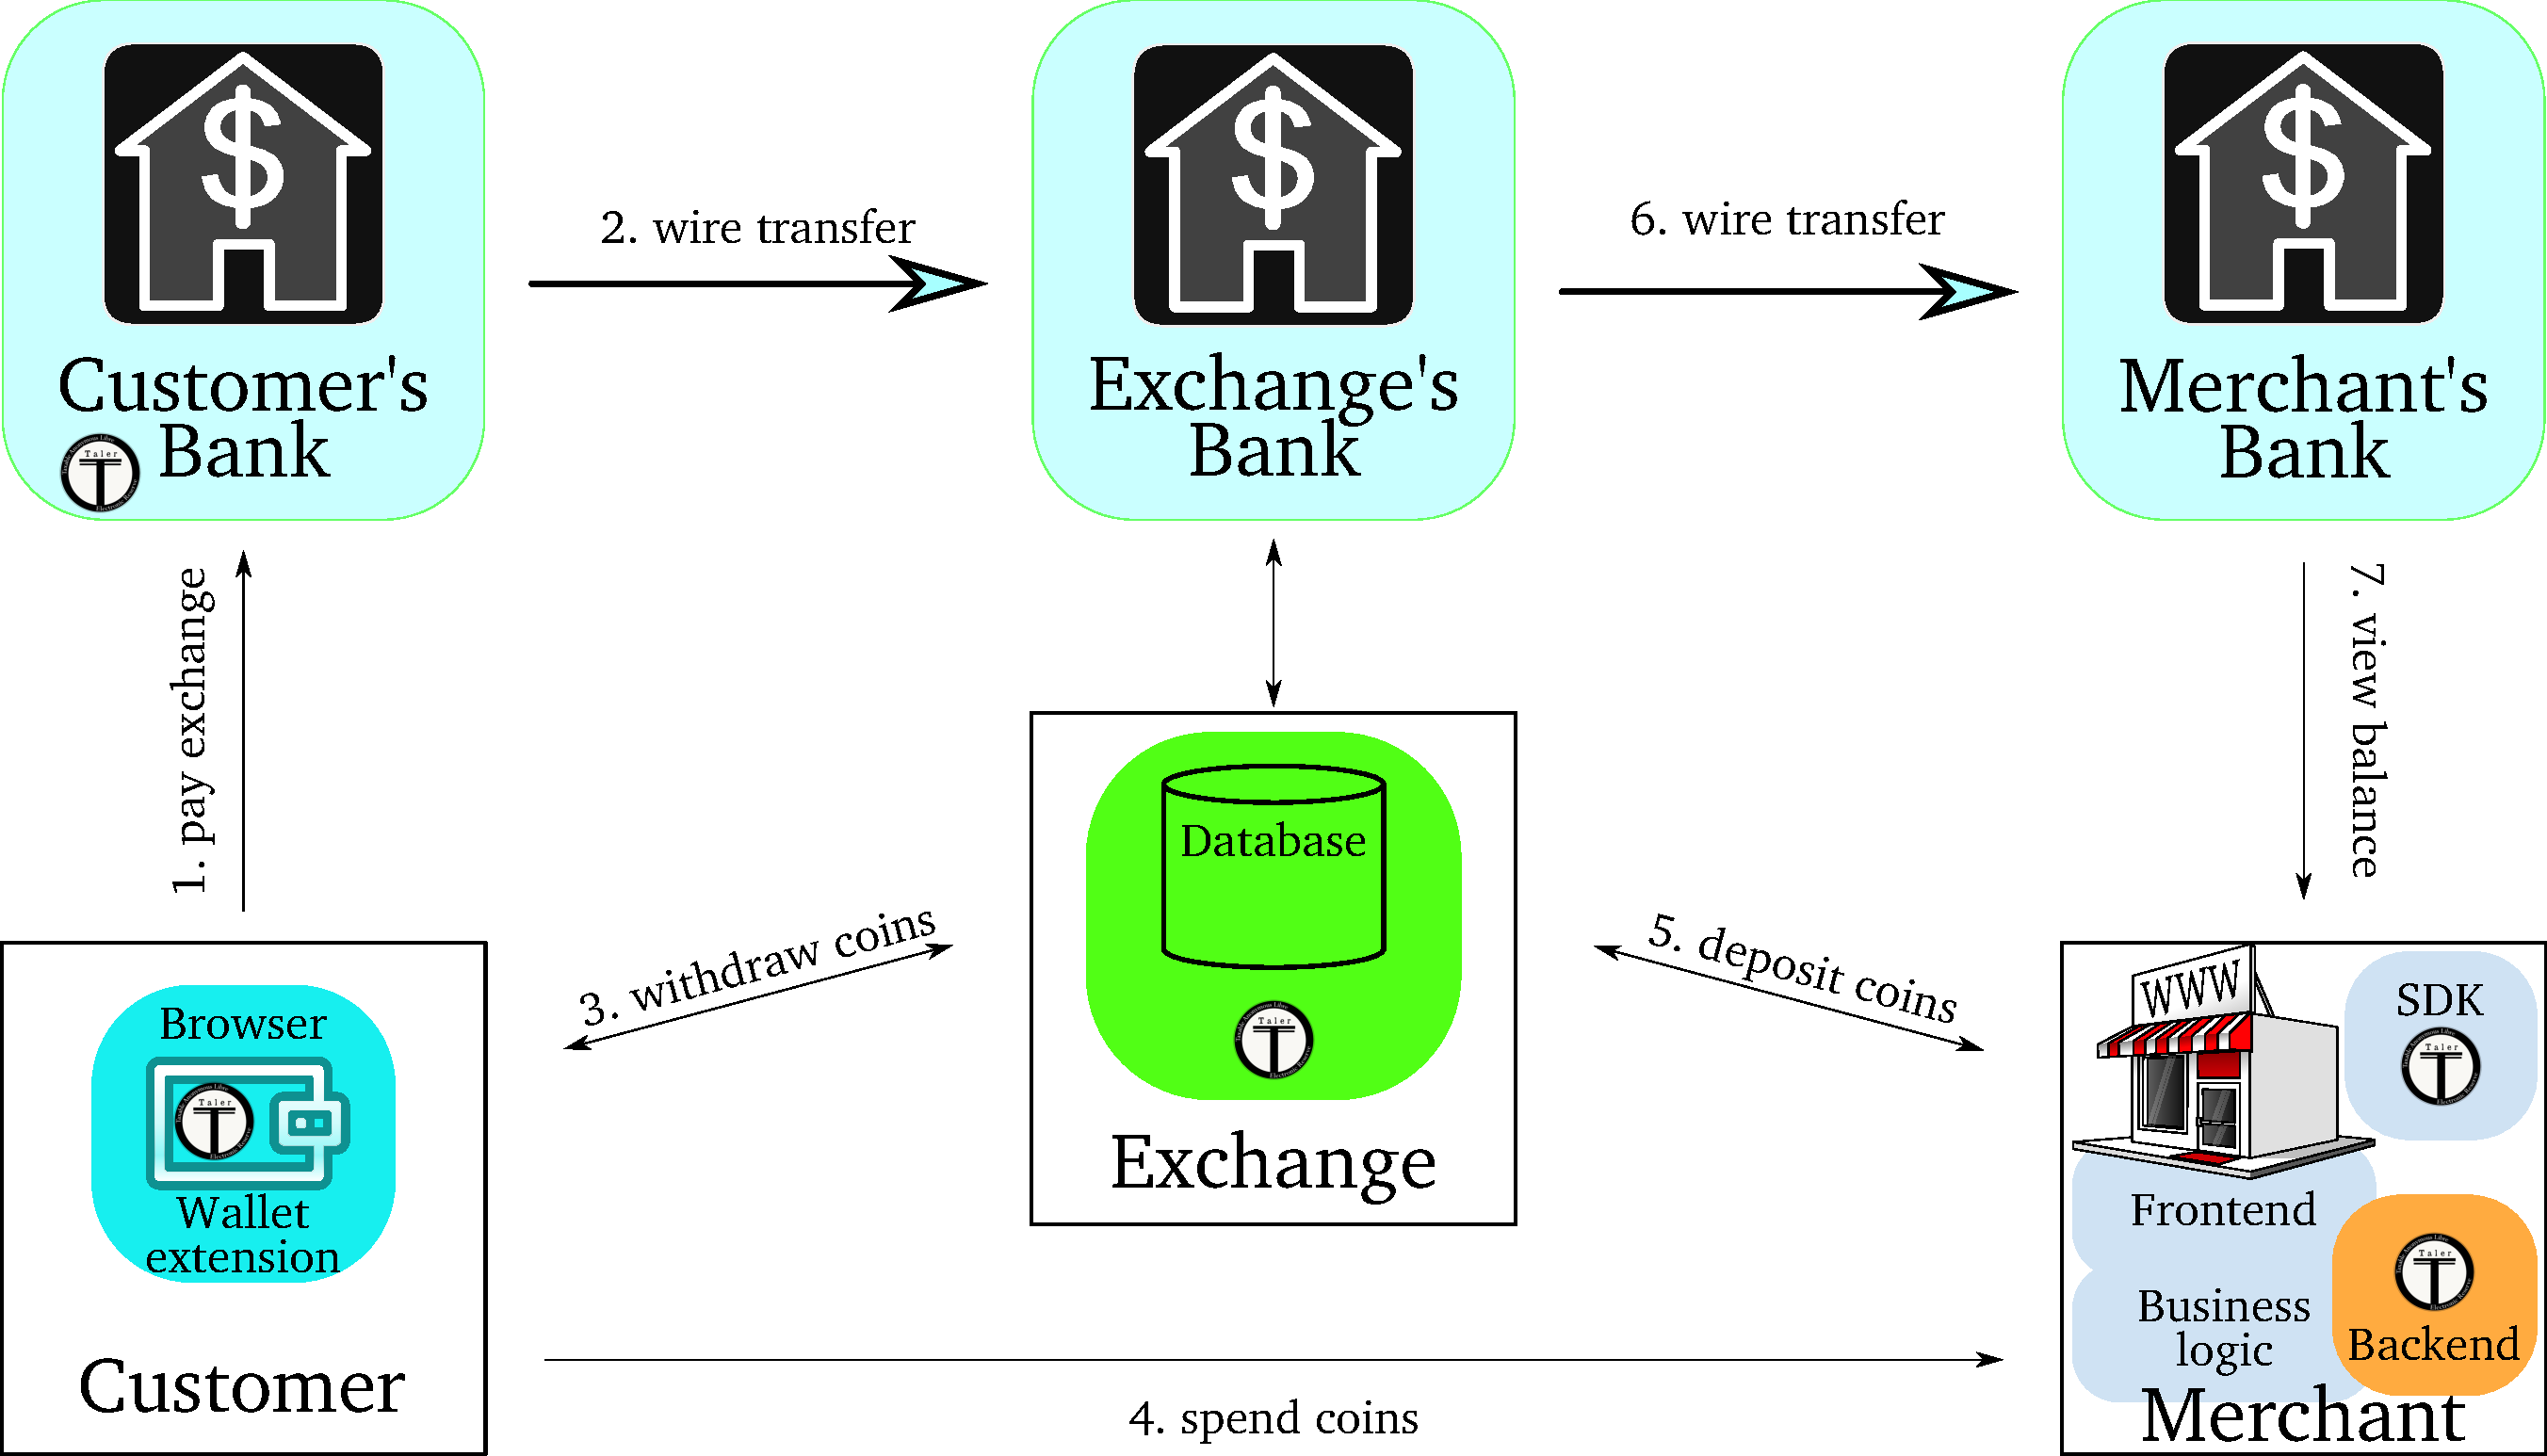
\includegraphics[width=\columnwidth]{taler-arch-full.pdf}
  \caption[Components of GNU Taler in the context of a banking system.]{The different components of the Taler system in the
    context of a banking system providing money creation,
    wire transfers and authentication. (Auditor omitted.)}
  \label{fig:taler-arch-full}
\end{figure}

As shown in Figure~\ref{fig:taler-arch-full}, the merchant is internally split
into multiple components.  The implementation of the Taler protocol and
cryptographic operations is isolated into a separate component, called the
\emph{merchant backend}, which the merchant accesses through an API or software
development kit (SDK) in the programming language of their choice.

Our implementations of the exchange (70,000 LOC) and merchant backend
(20,000 LOC) are written in C using PostgreSQL as the database and
libgcrypt for cryptographic operations.  The \emph{wallet} (10,000
LOC) is implemented in TypeScript as a cross-browser extension using
the WebExtensions API, which is available for a majority of widely
used browsers.  It also uses libgcrypt (compiled to JavaScript) for
cryptographic operations as the required primitives are not yet
natively supported by web browsers.  Sample merchant websites (1,000
LOC) and an example bank (2,000 LOC) with tight Taler integration are
provided in Python.

The code is available at \url{https://git.taler.net/} and a demo
is publicly available at \url{https://demo.taler.net/}.

\section{Overview}

We provide a high-level overview over the implementation,
before discussing the respective components in detail.

\subsection{Taler APIs}
The components of Taler communicate over an HTTP-based, RESTful\footnote{
Some REST purists might disagree, because the Taler APIs do not follow
all REST principles religiously.  In particular, the HATEOAS principle is not followed.
} \cite{fielding2000architectural}
API.  All request payloads and responses are JSON \cite{rfc8259} documents.

Binary data (such as key material, signatures and hashes) is encoded as a
base32-crockford \cite{crockford_base32} string. Base32-crockford is a simple,
case-insensitive encoding of binary data into a subset of the ASCII alphabet
that encodes 5 bits per character.  While this is not the most space-efficient
encoding, it is relatively resilient against human transcription errors.

Financial amounts are treated as fixed-point decimal numbers.  The
implementation internally uses a pair of integers $(v,f)$ with value part $0
\le v \le 2^{52}$ and fractional part $0 \le f < 10^8$ to represent the amount
$a = v + f\cdot 10^{-8}$.  This representation was chosen as the smallest
representable amount is equal to one Satoshi (the smallest representable amount
in Bitcoin), and the largest possible value part (besides being large enough
for typical financial applications) is still accurately representable in 64-bit
IEEE 754 floating point numbers.  These constraints are useful as some
languages such as JavaScript\footnote{Big integers are currently in the process
of being added to the JavaScript language standard.} provide IEEE 753 floating
point numbers as the only numeric type.  More importantly, fixed-point decimal
numbers allow exact representation of decimal values (say \EUR{0.10}), which
is not possible with floating point numbers but essential in financial applications.

Signatures are made over custom binary representations of the respective
values, prefixed with a 64-bit tag consisting of the size of the message (32
bits) and an integer tag (32 bits) uniquely identifying the purpose of the message.
To sign a free-form JSON object, a canonical representation as a string is
created by removing all white space and sorting objects' fields.

In the future, more space-efficient representations (such as BSON\footnote{http://bsonspec.org/} or CBOR \cite{rfc7049})
could be used.  The representation can be negotiated between client and server
in a backwards-compatible way with the HTTP ``Accept'' header.

% signatures!

\subsection{Cryptographic Algorithms}
The following cryptographic primitives are used by Taler:
\begin{itemize}
  \item SHA512 \cite{rfc4634} as a cryptographic hash function
  \item Ed25519 \cite{bernstein2006curve25519} for non-blind signing operations
  \item Curve25519 \cite{bernstein2006curve25519} for the refreshing operation
  \item HKDF \cite{rfc5869} as a key derivation function for the refreshing operation
  \item FDH-RSA blind signatures \cite{bellare2003onemore}
\end{itemize}

We chose these primitives as they are simple, cheap enough and relatively well
studied.  Note that other signature schemes that have the syntax and properties
described in Section~\ref{sec:crypto:instantiation}, such as
\cite{boldyreva2003threshold}, could be used instead of FDH-RSA.  

\subsection{Entities and Public Key Infrastructure}

\begin{figure}
    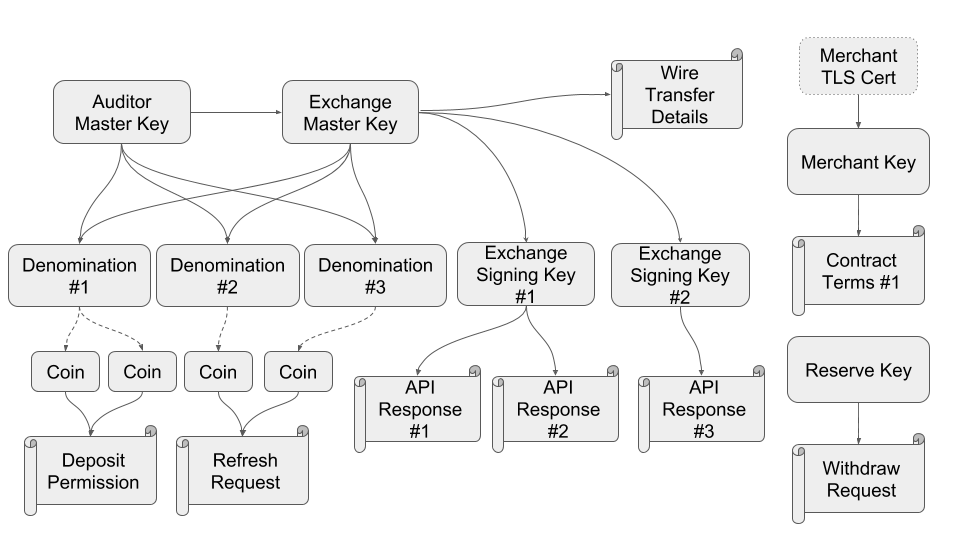
\includegraphics[width=\textwidth]{diagrams/taler-diagram-signatures.png}
    \caption[Entities/PKI in Taler]{Entities/PKI in Taler. Solid arrows denote signatures, dotted arrows denote blind signatures.}
\end{figure}

The public key infrastructure (PKI) used by Taler is orthogonal to the PKI used
by TLS \cite{rfc5246}.  While TLS is used as the transport layer for Taler API
messages, we do not rely on TLS for authenticity or integrity of API queries
and responses.  We do rely on TLS for the confidentiality of digital business
contracts and the authenticity, integrity and confidentiality of digital
product delivery.  For the anonymity properties to hold, the customer must
access the merchant and exchange through an anonymity layer (approximated
by practical implementations like Tor \cite{dingledine2004tor}).

In the case of merchants, we cannot use a trusted auditor or exchange as a
trust anchor, since merchants are not required to register within our PKI to
accept Taler payments.  Here we rely on TLS instead:  The merchant is required
to include their Taler-specific merchant public key in their TLS certificate.
If a merchant fails to do this, the wallet will show a warning when asking the
user to confirm a payment.

\subsubsection{Auditor}
Auditors serve as trust anchors for Taler, and are identified by a single Ed25519 public key.
Wallet implementations come with a pre-defined list of trusted auditors, similar to the certificate
store of browsers or operating systems.

\subsubsection{Exchange}
An exchange is identified by a long term Ed25519 master key and the exchange's
base URL.  The master key is used as an offline signing key, typically stored
on an air-gapped machine.  API requests to the exchange are made by appending
the name of the endpoint to the base URL.

The exchange uses the master key to sign the following data offline:
\begin{itemize}
  \item The exchange's online Ed25519 signing keys.  The online signing keys
    are used to sign API responses from the exchange.  Each signing key has a
    validity period.
  \item The denominations offered by the exchange (explained further in Section~\ref{sec:implementation:denoms}).
  \item The bank accounts supported by the exchange (for withdrawals and deposits) and associated fees.
\end{itemize}

% FIXME: maybe put this later?
The \texttt{<base-url>/keys} HTTP endpoint of the exchange is used by wallets
and merchants to obtain the exchange's signing keys, currently offered
denominations and other details.  In order to reduce traffic, clients can also
request only signing keys and denominations that were created after a specific
time.  The response to \texttt{/keys} is signed by a currently active signing
key, so that customers would have proof in case the exchange gave different sets of
denomination keys to different customers in an attempt to deanonymize them.


\begin{figure}
  \begin{multicols}{2}
  \lstinputlisting[language=C,basicstyle=\ttfamily\tiny,numbers=left]{taler/snippet-keys.txt}
  \end{multicols}
  \caption{Example response for /keys}
\end{figure}


\subsubsection{Coins and Denominations}\label{sec:implementation:denoms}

Denominations are the RSA public keys used to blindly sign coins of a fixed amount, together with information about their
validity and associated fees.  The following information is signed by the exchanges master key for every denomination:
\begin{itemize}
  \item The RSA public key.
  \item The start date, after which coins of this denomination can be withdrawn and deposited.
  \item The withdraw expiration date, after which coins cannot be withdrawn anymore, must be after the start date.
  \item The deposit expiration date, after which coins cannot be deposited anymore, must be after the withdraw expiration date.
  \item The legal expiration date, after which the exchange can delete all records about operations with coins of this denominations,
    must be (typically quite a long time!) after the deposit expiration date.
  \item The fees for a withdraw, deposit, refresh and refund operation with this coin, respectively.
\end{itemize}

\begin{figure}
    \centering
    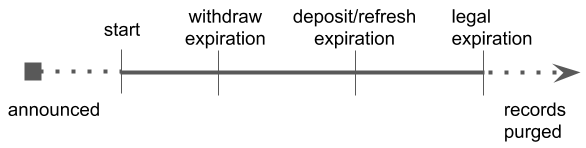
\includegraphics[width=0.7\textwidth]{diagrams/taler-diagram-denom-expiration.png}
    \caption{A denomination's lifetime.}
\end{figure}

An exchange can be audited by zero, one or multiple auditors.  An auditor must
monitor all denominations currently offered by the exchange, and an audit of a
subset of denominations is not intended in the current design.  To allow
customers of an exchange to confirm that it is audited properly, the auditor
signs an auditing request from the exchange, containing basic information about
the exchange as well as all keys offered during the auditing period.  In
addition to the full auditing request, the auditor also signs an individual
certificate for each denomination individually, allowing clients of the
exchange to incrementally verify newly offered denominations.

\subsubsection{Merchant}
The merchant has one Ed25519 key pair that is used to sign responses to the
customer and authenticate some requests to the exchange.  Depending on the
legislation that applies to a particular GNU Taler deployment, merchants might
not need to establish an a priori relationship with the exchange, but instead
send their bank account information during or after the first deposit of a
payment from a customer.

% FIXME: we never write here that the merchant accepts payments from all trusted auditors/exchanges
% automatically
% FIXME: citation for this?
% FIXME: are there jurisdictions where KYC would apply to the exchange's customer?
In some jurisdictions, exchanges are required to follow know-your-customer
(KYC) regulations and to verify the identity of merchants \cite{arner2018identity} using that particular
exchange for deposits.  Typically, the identity of a merchant only has to be
verified if a merchant exceeds a certain threshold of transactions in a given
time span.  As the KYC registration process can be costly to the exchange, this
requirement is somewhat at odds with merchants accepting payments from all
exchanges audited by a trusted auditor, since KYC registration needs to be done
at every exchange separately.  It is, however, unavoidable to run a legally
compliant payment system.

A merchant is typically configured with a set of trusted auditors and
exchanges, and consequently accepts payments with coins of denominations from a
trusted exchange and denominations audited by a trusted auditor.

In order to make the deployment of Taler easier and more secure, the parts that
deal with the merchant's private key and cryptographic operations are isolated
into a separate service (the merchant backend) with a well-defined RESTful HTTP API.
This concept is similar to payment gateways used commonly for credit card
payments.  The merchant backend can be deployed on-premise by the online shop,
or run by a third party provider that is fully trusted by the merchant.

\subsubsection{Bank}
Since the banks are third parties that are not directly part of Taler, they do
not participate directly in Taler's PKI.

\subsubsection{Customer}
Customers are not registered with an exchange, instead they use the private
keys of reserves that they own to authenticate with the exchange.  The exchange
knows the reserve's public key from the subject/instruction data of the wire
transfer.  Wire transfers that do not contain a valid public key are
automatically reversed.


\subsection{Payments}

\newlength{\maxheight}
\setlength{\maxheight}{\heightof{\small W}}
\newcommand{\bffmt}[1]{%
  \footnotesize
  \centering
  \raisebox{0pt}[\maxheight][0pt]{#1}%
}

\begin{figure}
\centering
\begin{bytefield}[bitwidth=0.2em,bitheight=3ex,boxformatting=\bffmt]{128}
  \bitheader{0,31,63,95,127} \\
  \bitbox{32}{size} & \bitbox{32}{purpose} & \bitbox{64}{timestamp} \\
  \wordbox{2}{merchant public key} \\
  \wordbox{4}{contract terms hash} \\
  \bitbox{64}{deposit deadline} & \bitbox{64}{refund deadline} \\
  \wordbox{4}{KYC / account info hash}
\end{bytefield}
\caption{The contract header that is signed by the merchant.}
\end{figure}

\begin{figure}
\centering
\begin{bytefield}[bitwidth=0.2em,bitheight=3ex,boxformatting=\bffmt]{128}
  \bitheader{0,31,63,95,127} \\
  \bitbox{32}{size} & \bitbox{32}{purpose} & \bitbox{64}{timestamp} \\
  \wordbox{4}{contract header hash} \\
  \wordbox{2}{coin public key} \\
  \bitbox[lrt]{128}{contributed amount} \\
  \bitbox[lrb]{64}{} & \bitbox[ltr]{64}{} \\
  \bitbox[lrb]{128}{deposit fee} \\
\end{bytefield}
\caption{The deposit permission signed by the customer's wallet.}
\end{figure}


Payments in Taler are based on \emph{contract terms}, a JSON object that
describes the subject and modalities of a business transaction.  The
cryptographic hash of such a contract terms object can be used as a globally
unique identifier for the business transaction.  Merchants must sign the
contract terms before sending them to the customer, allowing a customer to
prove in case of a dispute the obligations of the merchant resulting from the
payment.

Unless a third party needs to get involved in a dispute, it is sufficient (and
desirable for data minimization) that only the merchant and the customer know
the full content of the contract terms.  The exchange, however,  must still
know the parts of the contract terms that specify payment modalities, such as
the refund policy, micropayment aggregation deadline and the merchant's KYC
registration data (typically a hash to prove the KYC enrollment of the
merchant).

Thus, the merchant's signature is made over the \emph{contract header},
which contains the contract terms hash, as well as the payment modalities.

In addition to the data provided by the merchant, the contract terms contain a
\emph{claim\_pub} field whose value is provided by the customer.
This field is an Ed25519 public key, and the customer can use the corresponding
private key to prove that they have indeed obtained the individual contract
terms from the merchant, and did not copy contract terms that the merchant gave
to another customer.  Note that this key is not a permanent identity of the
customer, but should be freshly generated for each payment.

The signed contract header is created by the merchant's backend from an
\emph{order}, which is the ``blueprint'' for the contract terms.  The order is
generated by the merchant's frontend and contains a subset of the data
contained in the contract terms.  Missing data (in particular the merchant's
bank account information, public key and accepted auditors/exchanges) and
the claim public key obtained from the customer is automatically added by the merchant
backend.  This allows applications to process payments without having to
specify Taler-internal details.  In fact, the smallest possible order only
needs to contain two fields:  the amount to be paid and a human-readable
summary of the payment's subject.

An order contains an \emph{order ID}, which is an identifier that is unique
within a given merchant and can be a human-friendly identifier such as a
booking number.  If the order ID is not manually provided, it is automatically
filled in by the merchant backend.  It can be used to refer to the payment
associated with the order without knowing the contract terms hash, which is
only available once the customer has provided their claim public key.

To initiate a payment, the merchant sends the customer an \emph{unclaimed}
contract terms URL.  The customer can download and thereby claim ownership of
the contract by appending their claim public key $p$ as a query parameter to the unclaimed
contract terms URL and making an HTTP \texttt{GET} request to the resulting URL.
The customer must then verify that the resulting contract terms are signed
correctly by the merchant and that the contract terms contain their claim public key $p$.
A malicious customer could try to claim other customers' contracts by guessing
contract term URLs and appending their own claim public key.  For products that have
limited availability, the unclaimed contract URL must have enough entropy so
that malicious customers are not able to guess them and claim them before the
honest customer.\footnote{Note that this URL cannot be protected by a session
cookie, as it might be requested from a different session context than the
user's browser, namely in the wallet.}

% FIXME: put this in a sidebox?
To give an example, an online shop for concert tickets might allow users to put
themselves on a waiting list, and will send them an email once a ticket
becomes available.  The contract terms URL that allows the customer to purchase
the ticket (once they have visited a link in this email), should contain an
unguessable nonce, as otherwise an attacker might be able to predict the URL
and claim the contract for the concert ticket before the customer's wallet can.

In order to settle the payment, the customer must sign a \emph{deposit
permission} for each coin that comprises the payment.  The deposit permission
is a message signed by the coin's private key, containing
\begin{itemize}
  \item the amount contributed by this coin to the payment,
  \item the merchant's public key
  \item the contract header together with the merchant's signature on it,
  \item the time at which the deposit permission was signed.
\end{itemize}

After constructing the deposit permissions for a contract, the customer sends
them to the merchant by doing an HTTP \texttt{POST} request to the
\texttt{pay\_url} indicated by the merchant in the contract terms.  The
merchant individually \emph{deposits} each deposit permission with the
exchange.

The merchant responds with a payment confirmation to the customer after it has
successfully deposited the customer's coins with the exchange.  The payment
confirmation can be used by the customer to prove that they completed the
payment before the payment deadline indicated in the contract terms.

Note that the depositing multiple coins with the exchange deliberately does not
have transactional semantics.  Instead, each coin is deposited in an individual
transaction.  This allows the exchange to be horizontally scaled (as discussed
in Section~\ref{sec:implementation-improvements}) more easily, as deposit
transaction might otherwise have to span multiple database shards.

The lack of transactional semantics, however, means that it must be possible to
recover from partially completed payments.  There are several cases: If one of
the coins that the customer submitted as payment to the merchant is invalid
(e.g., because the wallet's state was restored from a backup), the customer can
re-try the partially completed payment and provide a different coin instead.
If that is not possible or desired by the customer, the merchant may voluntarily give a
refund on the coins that have been previously deposited.  The reference
implementation of the merchant backend offers refunds for partially completed
payments automatically.

% FIXME: explain why!
If refunds were disabled for the payment, the merchant does not cooperate in
giving refunds for a partially completed payment, or becomes unresponsive after
partially depositing the customer's coin, the customer has two options: They
can either complete the deposits on the merchant's behalf, and then use the
deposit permissions to prove (either to the merchant or to a court) that they
completed the payment.

% FIXME: put this in info box?
Another possibility would be to allow customers to request refunds for partially
completed payments themselves, directly from the exchange.
This requires that the merchant additionally
includes the amount to be paid for the contract in the contract header, as the
exchange needs to know that amount to decide if a payment with multiple coins
is complete.  We do not implement this approach, since it implies that the
exchange always learns the exact prices of products that the merchant sells, as
opposed to just the merchant's total revenue.

The customer could also reveal the contract terms to the exchange to prove that
a payment is incomplete, but this is undesirable for privacy reasons, as the
exchange should not learn about the full details of the business agreement
between customer and merchant.

\subsection{Resource-based Web Payments}
In order to integrate natively with the concepts and architecture of the web,
Taler supports paying for a web resource in the form of a URL.  In fact all
Taler contract terms contain a \emph{fulfillment URL}, which identifies the
resource that is being paid for.  If the customer is not paying for a digital
product (such as an movie, song or article), the fulfillment URL can point to a
confirmation page that shows further information, such as a receipt for a
donation or shipment tracking information for a physical purchase.  A
fulfillment URL does not necessarily refer to a single item, but could also
represent a collection such as a shopping basket.

The following steps illustrate a typical payment with the online shop
\nolinkurl{alice-shop.example.com}.

\newcommand{\contl}[0]{\mbox{\textcolor{blue}{$\hookrightarrow$}\space}}

\lstdefinelanguage{none}{
  identifierstyle=
}
\lstdefinestyle{myhttp}{
  breaklines=true,
  breakindent=3em,
  escapechar=*,
  postbreak=\contl,
  basicstyle=\ttfamily,
  showspaces=true,
}

\begin{enumerate}
  \item The user opens the shop's page and navigates to a paid resource, such
    as \nolinkurl{https://alice-shop.example.com/essay-24.pdf}.
  \item The shop sends a response with HTTP status ``402 Payment Required''
    with the headers (\contl marks a continued line)
\begin{lstlisting}[style=myhttp]
Taler-Contract-Url: https://alice-shop.example.com/*\break\contl*contract?product=essay-24.pdf
Taler-Resource-Url: https://alice-shop.example.com/*\break\contl*essay-24.pdf
\end{lstlisting}
  \item Since the user's wallet does not yet contain contract terms with the
    fulfillment URL \nolinkurl{https://alice-shop.example.com/esasy-24.pdf}
    that matches the resources URL, it claims the contract by generating a
    claim key pair $(s, p)$  and requesting the contract URL with the claim
    public key $p$ as additional parameter:
    \nolinkurl{https://alice-shop.example.com/contract?product=essay-24.pdf\&claim_pub=}$p$.
  \item The wallet displays the contract terms to the customer and asks them to
    accept or decline.  If the customer accepted the contract, the wallet sends
    a payment to the merchant.  After the merchant received a valid payment,
    it marks the corresponding order as paid.
  \item The wallet constructs the extended fulfillment URL by adding the order
    id from the contract as an additional parameter and navigates the browser
    to the resulting URL
    \nolinkurl{https://alice-shop.example.com/esasy-24.pdf?order\_id=...}.
  \item The shop receives the request to the extended fulfillment URL and
    checks if the payment corresponding to the order ID was completed.  In case
    the payment was successful, it serves the purchased content.
\end{enumerate}

To avoid checking the status of the payment every time, the merchant can
instead set a session cookie (signed/encrypted by the merchant) in the user's
browser which indicates that \texttt{essay-24.pdf} has been purchased.

The resource-based payment mechanism must also handle the situation where a
customer navigates again to a resource that they already paid for, without
directly navigating to the extended fulfillment URL.  In case no session cookie
was set for the purchase or the cookie was deleted / has expired, the customer would
be prompted for a payment again.  To avoid this, the wallet tries to find an
existing contract whose plain fulfillment URL matches the resource URL
specified in the merchant's HTTP 402 response.  If such an existing payment was
found, the wallet instead redirects the user to the extended fulfillment URL
for this contract, instead of downloading the new contract terms and prompting
for payment.

In the example given above, the URL that triggers the payment is the same as the fulfillment URL.
This may not always the case in practice.  When the merchant backend is hosted by a third
party, say \nolinkurl{https://bob.example.com/}, the page that triggers the payment
even has a different origin, i.e., the scheme, host or port may differ \cite{rfc6454}.

This cross-origin operation presents a potential privacy risk if not
implemented carefully.
To check whether a user has already paid for a particular
resource with URL $u$, an arbitrary website could send an HTTP 402 response with
the ``Taler-Resource-Url'' header set to $u$ and the ``Taler-Contract-Url''
set to a URL pointing to the attacker's server.  If the user paid for $u$, the
wallet will navigate to the extended fulfillment URL corresponding to $u$.
Otherwise, the wallet will try to download a contract from the URL given by the
attacker.  In order to prevent this attack on privacy, the wallet must only
redirect to $u$ if the origin of the page responding with HTTP 402 is the same
origin as either the $u$ or the pay URL.\footnote{This type of countermeasure is well
known in browsers as the same origin policy, as also outlined in \cite{rfc6454}.}

\subsubsection{Loose Browser Integration}\label{sec:loose-browser-integration}

The payment process we just described does not directly work in browsers that do not
have native Taler integration, as the browser (or at least a browser extension)
would have to handle the HTTP status code 402 and handle the Taler-specific headers correctly.
We now define a fallback, which is transparently implemented in the reference merchant backend.

In addition to indicating that a payment is required for a resource in the HTTP status code and header,
the merchant includes a fallback URL in the body of the ``402 Payment Required'' response.  This URL must have the custom URL scheme
\texttt{taler}, and contains the contract terms URL (and other Taler-specific settings normally specified in headers)
as parameters.  The above payment would include a link (labled, e.g., ``Pay with GNU Taler'') to the following URL, encoding
the same information as the headers:
\begin{lstlisting}[style=myhttp]
taler:pay?*\break\contl*contract_url=*\break\contl*https%3A%2F%2Falice-shop.example.com%2Fcontract%3Fproduct%3Dessay-24.pdf*\break\contl*&resource_url=*\break\contl*https%3A%2F%2Falice-shop.example.com%2Fessay-24.pdf
\end{lstlisting}

This fallback can be disabled for requests from user agents that are known to
natively support GNU Taler.

GNU Taler wallet applications register themselves as a handler for the
\texttt{taler} URI scheme, and thus following a \texttt{taler:pay} link opens
the dedicated wallet, even if GNU Taler is not supported by the browser or a
browser extension.  Registration a custom protocol handler for a URI scheme is
possible on all modern platforms with web browsers that we are aware of.

Note that wallets communicating with the merchant do so from a different
browsing context, and thus the merchant backend cannot rely on cookies that
were set in the customer's browser when using the shop page.

We chose HTTP headers as the primary means of signaling to the wallet (instead
of relying on, e.g., a new content media type), as it allows the fallback content
to be an HTML page that can be rendered by all browsers. Furthermore,
current browser extension mechanism allow intercepting headers synchronously
before the rendering of the page is started, avoiding visible flickering caused by
intermediate page loads.

\subsection{Session-bound Payments and Sharing}
As we described the payment protocol so far, an extended fulfillment URL
is
not bound to a browser session.  When sharing an extended fulfillment
URL, another user would get access to the same content.  This might be appropriate
for some types of fulfillment pages (such as a donation receipt), but is generally not
appropriate when digital content is sold.  Even though it is trivial to share digital content
unless digital restrictions management (DRM) is employed, the ability to share
links might set the bar for sharing too low.

While the validity of a fulfillment URL could be limited to a certain time,
browser session or IP address, this would be too restrictive for scenarios where
the user wants to purchase permanent access to the content.

As a compromise, Taler provides \emph{session-bound} payments.  For
session-bound payments, the seller's website assigns the user a random session
ID, for example, via a session cookie.  The extended fulfillment URL for
session-bound payments is constructed by additionally specifying the URL
parameter \texttt{session\_sig}, which contains proof that the user completed
(or re-played) the payment under their current session ID.

To initiate a session-bound payment, the HTTP 402 response must additionally
contain the ``Taler-Session-Id'' header, which will cause the wallet to
additionally obtain a signature on the session ID from the merchant's pay URL,
by additionally sending the session ID when executing (or re-playing) the
payment.
As an optimization, instead of re-playing the full payment, the wallet can also
send the session ID together with the payment receipt it obtained from the
completed payment with different session ID.

Before serving paid content to the user, the merchant simply checks if the
session signature matches the assigned session and contract terms.  To simplify
the implementation of the frontend, this signature check can be implemented as
a request to the GNU Taler backend.  Using session signatures instead of storing
all completed session-bound payments in the merchant's database saves storage.

While the coins used for the payment or the payment receipt could be shared
with other wallets, it is a higher barrier than just sharing a URL.  Furthermore, the
merchant could restrict the rate at which new sessions can be created for the
same contract terms and restrict a session to one IP address, limiting sharing.

For the situation where a user accesses a session-bound paid resource and
neither has a corresponding contract in their wallet nor does the merchant
provide a contract URL to buy access to the resource, the merchant can specify
an \emph{offer URL} in the ``Taler-Offer-Url'' header.  If the wallet is not
able to take any other steps to complete the payment, it will redirect the user
to the offer URL.  As the name suggests, the offer URL can point to a page with
alternative offers for the resource, or some other explanation as to why the
resource is not available anymore.

\subsection{Embedded Content}
So far we only considered paying for a single, top-level resource,
namely the fulfillment URL.  In practice, however, websites are composed of
many subresources such as embedded images and videos.

We describe two techniques to ``paywall'' subresources behind a GNU Taler
payment.  Many other approaches and variations are possible.
\begin{enumerate}
  \item Visiting the fulfillment URL can set a session cookie.  When a
    subresource is requested, the server will check that the customer has the
    correct session cookie set.
  \item When serving the fulfillment page, the merchant can add an additional
    authentication token to the URLs of subresources.  When the subresource is
    requested, the validity of the authentication token is checked.  If the
    merchant itself (instead of a Content Delivery Network that supports token
    authentication) is serving the paid subresource, the order ID and session
    signature can also be used as the authentication token.
\end{enumerate}

It would technically be possible to allow contract terms to refer to multiple
resources that are being purchased by including a list or pattern that defines
a set of URLs.  The browser would then automatically include information to
identify the completed payment in the request for the subresource.  We
deliberately do not implement this approach, as it would require deeper
integration in the browser than possible on many platforms.  If not restricted
carefully, this feature could also be used as an additional method to track the
user across the merchant's website.

\subsection{Contract Terms}
The contract terms, only seen by the customer and the merchant (except when a tax audit of the merchant is requested)
contain the following information:
\begin{itemize}
  \item The total amount to be paid,
  \item the \texttt{pay\_url}, an HTTP endpoint that receives the payment,
  \item the deadline until the merchant accepts the payment (repeated in the signed contract header),
  \item the deadline for refunds (repeated in the signed contract header),
  \item the claim public key provided by the customer, used to prove they have claimed the contract terms,
  \item the order ID, which is a short, human-friendly identifier for the contract terms within
    the merchant,
  \item the \texttt{fulfillment\_url}, which identifies the resources that is being paid for,
  \item a human-readable summary and product list,
  \item the fees covered by the merchant (if the fees for the payment exceed this value, the
    customer must explicitly pay the additional fees),
  \item depending on the underlying payment system, KYC registration information
    or other payment-related data that needs to be passed on to the exchange (repeated in the signed contract header),
  \item the list of exchanges and auditors that the merchants accepts for the payment,
  \item information about the merchant, including the merchant public key and contact information.
\end{itemize}


\subsection{Refunds}
By signing a \emph{refund permission}, the merchant can ``undo'' a deposit on a
coin, either fully or partially.  The customer can then spend (or refresh) the
refunded value of the coin again.  A refund is only possible before the refund
deadline (specified in the contract header).  After the refund deadline has
passed (and before the deposit deadline) the exchange makes a bank transfer the
merchant with the aggregated value from deposits, a refund after this point
would require a bank transfer back from the merchant to the exchange.

Each individual refund on each coin incurs fees; the
refund fee is subtracted from the amount given back to the customer and kept by
the exchange.

Typically a refund serves either one of the following purposes:
\begin{itemize}
  \item An automatic refund is given to the customer when a payment only
    partially succeeded.  This can happen when a customer's wallet accidentally
    double-spends, which is possible even with non-malicious customers and caused by data
    loss or delayed/failed synchronization between the same user's wallet on
    multiple devices.  In these cases, the user can choose to re-try the
    payment with different, unspent coins (if available) or to ask for a refund
    from the merchant.
  \item A voluntary refund can be given at the discretion of the merchant,
    for example, when the customer is not happy with their purchase.
\end{itemize}
Refunds require a signature by the merchant, but no consent from the customer.

A customer is notified of a refund with the HTTP 402 Payment Required status
code and the ``Taler-Refund'' header.  The value of the refund header is a
URL. An HTTP \texttt{GET} request on that URL will return a list of refund confirmations that the
merchant received from the exchange.

\subsection{Tipping}
Tipping in Taler uses the ``withdraw loophole'' (see \ref{taler:design:tipping}) to allow the
merchant\footnote{We still use the term ``merchant'', since donations use the same software component
as the merchant, but ``donor'' would be more accurate.} to donate small amounts (without any associated contract terms or legal
obligations) into the user's wallet.

To be able to give tips, the merchant must create a reserve with an exchange.  The reserve private key
is used to sign blinded coins generated by the user that is being given the tip.

The merchant triggers the wallet by returning an HTTP 402 Payment Required
response that includes the ``Taler-Tip'' header. The value of the tip header (called the
tip token) contains
\begin{itemize}
  \item the amount of the tip,
  \item the exchange to use,
  \item a URL to redirect after processing the tip,
  \item a deadline for picking up the tip,
  \item a merchant-internal unique ID for the tip, and
  \item the \emph{pickup URL} for the tip.
\end{itemize}
Upon receiving the tip token, the wallet creates coin planchets that sum up to at most
the amount specified in the tip token, with denominations offered by the exchange specified in the tip token.

The list of planchets is then sent to the merchant via an HTTP \texttt{POST}
request to the tip-pickup URL.  The merchant creates a withdrawal confirmation
signature for each planchet, using the private key of the tipping reserve, and
responds to the HTTP \texttt{POST} request with the resulting list of
signatures.  The user then uses these signatures in the normal withdrawal
protocol with the exchange to obtain coins ``paid for'' by the merchant, but
anonymized and only spendable by the customer.


\section{Bank Integration}
In order to use Taler for real-world payments, it must be integrated with the
existing banking system.  Banks can choose to tightly integrate with Taler and
offer the ability to withdraw coins on their website.  Even existing banks can
be used to withdraw coins via a manual bank transfer to the exchange, with the
only requirement that the 52 character alphanumeric, case-insensitive encoding
of the reserve public key can be included in the transaction without
modification other than case folding and white space
normalization.\footnote{Some banking systems specify that the subject of the
can be changed, and provide an additional machine-readable ``instruction''
field.  }

\subsection{Wire Method Identifiers}\label{implementation:wire-method-identifiers}
We introduce a new URI scheme \texttt{payto}, which is used in Taler to
identify target accounts across a wide variety of payment systems with uniform
syntax.

In in its simplest form, a \texttt{payto} URI identifies one account of a particular payment system:

\begin{center}
  \texttt{'payto://' TYPE '/' ACCOUNT }
\end{center}

When opening a \texttt{payto} URI, the default action is to open an application
that can handle payments with the given type of payment system, with the target
account pre-filled.  In its extended form, a \texttt{payto} URL can also specify
additional information for a payment in the query parameters of the URI.

In the generic syntax for URIs, the payment system type corresponds to the
authority, the account corresponds to the path, and additional parameters for
the payment correspond to the query parameters.  Conforming to the generic URI
syntax makes parsing of \texttt{payto} URIs trivial with existing parsers.

Formally, a \texttt{payto} URI is an encoding of a partially filled out pro
forma invoice.  The full specification of the \texttt{payto} URI is RFC XXXX. % FIXME!

In the implementation of Taler, \texttt{payto} URIs are used in various places:
\begin{enumerate}
  \item The exchange lists the different ways it can accept money as \texttt{payto} URIs.
    If the exchange uses payment methods that do not have tight Taler integration.
  \item In order to withdraw money from an exchange that uses a bank account type that
    does not typically have tight Taler integration, the wallet can generate a link and a QR code
    that already contains the reserve public key.  When scanning the QR code with a mobile device that
    has an appropriate banking app installed, a bank transfer form can be pre-filled and the user only has to confirm the
    transfer to the exchange.
  \item The merchant specifies the account it wishes to be paid on as a \texttt{payto} URI, both in
    the configuration of the merchant backend as well as in communication with the exchange.
\end{enumerate}

A major advantage of encoding payment targets as URIs is that URI schemes can be registered
with an application on most platforms, and will be ``clickable'' in most applications and open the right
application when scanned as a QR code.  This is especially useful for the first use case listed above; the other use cases
could be covered by defining a media type instead \cite{rfc6838}.

% FIXME: put into side box
As an example, the following QR code would open a banking application that supports SEPA payments,
pre-filled with a 15\EUR{} donation to the bank account of GNUnet:

\begin{center}
\qrcode[hyperlink,height=5em]{payto://sepa/DE67830654080004822650?amount=EUR:15}
\end{center}

\subsection{Demo Bank}
For demonstration purposes and integration testing, we use our toy bank
implementation\footnote{\url{https://git.taler.net/bank.git}}, which might be
used in the future for regional currencies or accounting systems (e.g., for a
company cafeteria).  The payment type identifier is \texttt{taler-bank}.  The
authority part encodes the base URL of the bank, and the path must be the
decimal representation of a single integer between $1$ and $2^{52}$, denoting
the internal demo bank account number.

\subsection{EBICS and SEPA}
The Electronic Banking Internet Communication Standard\footnote{\url{http://www.ebics.org}} (EBICS) is a standard
for communicating with banks, and is widely used in Germany, France and
Switzerland, which are part of the Single European Payment Area (SEPA).  EBICS
itself is just a container format.  A commonly supported payload for EBICS is
ISO 2022, which defines messages for banking-related business processes.

Integration of GNU Taler with EBICS is currently under development, and would
allow Taler to be easily deployed in many European countries, provided that the
exchange provider can obtain the required banking license.

\subsection{Blockchain Integration}
Blockchains such as Bitcoin could also be used as the underlying financial
system for GNU Taler, provided that merchants and customers trust the exchange to be honest.

With blockchains that allow more complex smart contracts, the auditing
functionality could be implemented by the blockchain itself.  In particular,
the exchange can be incentivized to operate correctly by requiring an initial
safety deposit to the auditing smart contract, which is distributed to
defrauded participants if misbehavior of the exchange is detected.

\section{Exchange}

\begin{figure}
    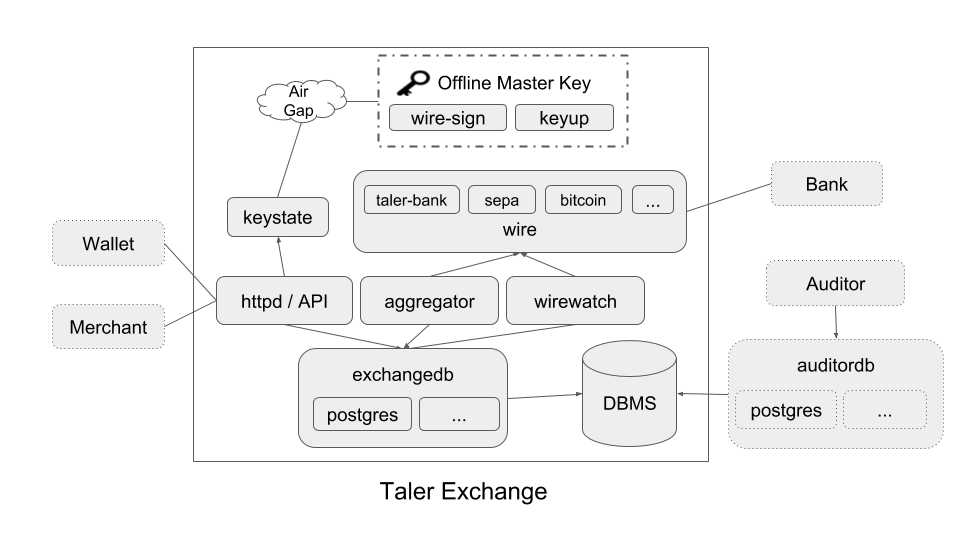
\includegraphics[width=\textwidth]{diagrams/taler-diagram-exchange.png}
    \caption{Architecture of the exchange reference implementation}
\end{figure}

The exchange consists of three independent processes:
\begin{itemize}
  \item The \texttt{taler-exchange-httpd} process handles HTTP requests from clients,
  mainly merchants and wallets.
  \item The \texttt{taler-exchange-wirewatch} process watches for wire transfers
  to the exchange's bank account and updates reserves based on that.
  \item The \texttt{taler-exchange-aggregator} process aggregates outgoing transactions
  to merchants.
\end{itemize}
All three processes exchange data via the same database.  Only
\texttt{taler-exchange-httpd} needs access to the exchanges online signing keys
and denomination keys.

The database is accessed via a Taler-specific database abstraction layer.
Different databases can be supported via plugins; at the time of writing this,
only a PostgreSQL plugin has been implemented.

Wire plugins are used as an abstraction to access the account layer that Taler
runs on.  Specifically, the \textit{wirewatch} process uses the plugin to monitor
incoming transfers, and the aggregator process uses the wire plugin to make
wire transfers to merchants.

The following APIs are offered by the exchange:
\begin{description}
  \item[Announcing keys, bank accounts and other public information]  The
    exchange offers the list of denomination keys, signing keys, auditors,
    supported bank accounts, revoked keys and other general information needed
    to use the exchange's services via the \texttt{/keys} and \texttt{/wire}
    APIs.
  \item[Obtaining entropy] As we cannot be sure that all client-devices have
    an adequate random number generator, the exchange offers the \texttt{/seed}
    endpoint to download some high-entropy value.  Clients should mix this
    seed with their own, locally-generated entropy into an entropy pool.
  \item[Reserve status and withdrawal] After having wired money to the exchange,
    the status of the reserve can be checked via the \texttt{/reserve/\$RESERVE\_PUB/status} API.  Since
    the wire transfer usually takes some time to arrive at the exchange, wallets should periodically
    poll this API, and initiate a withdrawal with \texttt{/reserve/\$RESERVE\_PUB/withdraw} once the exchange received the funds.
  \item[Deposits and tracking]  Merchants transmit deposit permissions they have received from customers
    to the exchange via the \texttt{/coins/\$COIN\_PUB/deposit} API.  Since multiple deposits are aggregated into one wire transfer,
    the merchant additionally can use the exchange's \texttt{/transfers/\$WTID} API that returns the list of deposits for a wire transfer
    identifier (WTID) included in the wire transfer to the merchant, as well as the \texttt{/deposits/\$H\_WIRE/\$MERCHANT\_PUB/\$H\_CONTRACT\_TERMS/\$COIN\_PUB} API to look up
    which wire transfer included the payment for a given deposit.
  \item[Refresh] Refreshing consists of two stages. First, using \texttt{/coins/\$COIN\_PUB/melt} an old, possibly dirty coin is melted and thus devaluted. The committment made by the wallet during the melt and the resulting $\gamma$-challenge from the exchange are associated with a {\em refresh session}.  Then, using \texttt{/refreshes/\$RCH/reveal} the wallet can answer the challenge and obtain fresh coins as change.  Finally, \texttt{/coins/\$COIN\_PUB/link} provides the link deterrent against refresh abuse.
  \item[Refunds] The refund API (\texttt{/coins/\$COIN\_PUB/refund}) can ``undo'' a deposit if the merchant gave their signature, and the aggregation deadline
    for the payment has not occurred yet.
  \item[Recoup]  The recoup API (\texttt{/coins/\$COIN\_PUB/recoup}) allows customers to be compensated
    for coins whose denomination key has been revoked.  Customers must send either a full withdrawal transcript that
    includes their private blinding factor, or a refresh transcript (of a refresh that had the revoked denominations as one of the targets)
    that includes blinding factors.  In the former case, the reserve is credited, in the latter case, the source coin of the
    refresh is refunded and can be refreshed again.
\end{description}

New denomination and signing keys are generated and signed with the exchange's master
secret key using the \texttt{taler-exchange-keyup} utility, according to a key schedule
defined in the exchange's configuration.  This process should be done on an air-gapped
offline machine that has access to the exchange's master signing key.

Generating new keys with \texttt{taler-exchange-keyup} also generates an
auditing request file, which the exchange should send its auditors.  The auditors then
certify these keys with the \texttt{taler-auditor-sign} tool.

\begin{figure}
    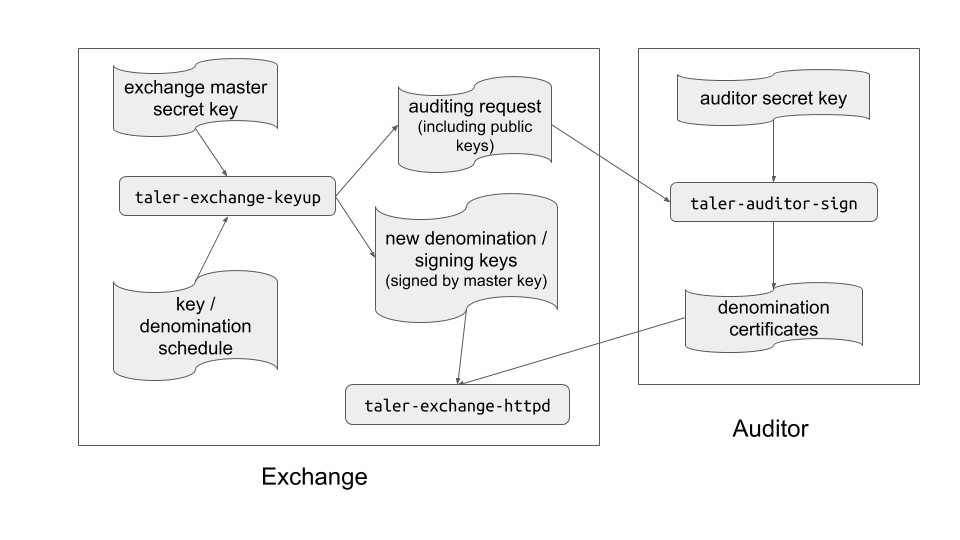
\includegraphics[width=\textwidth]{diagrams/taler-diagram-keyup.png}
    \caption{Data flow for updating the exchange's keys.}
    \label{figure:keyup}
\end{figure}

This process is illustrated in Figure~\ref{figure:keyup}.


\section{Auditor}

The auditor consists of several main components:
\begin{itemize}
 \item the \texttt{taler-auditor-dbinit} tool to setup,
   upgrade or garbage-collect an auditor's database,
 \item the \texttt{taler-auditor-exchange} tool to add an
   exchange to the list of audited exchanges,
 \item the \texttt{taler-auditor-sign} tool to sign an exchange's
   keys to affirm that the auditor is auditing this exchange,
 \item an HTTP service (\texttt{taler-auditor-httpd}) which
   receives deposit confirmations from merchants, and
 \item the \texttt{taler-auditor} script which must be regularly
   run to generate audit reports.
\end{itemize}

\subsection{Database synchronization}

FIXME: describe issue of how to synchronize exchange and auditor
databases, and how we solved it (once we did solve it!) here.

\subsection{The \texttt{taler-auditor} tool}

The \texttt{taler-auditor} script uses several helper processes.  These helper
processes access the exchange's database, either directly (for
exchange-internal auditing as part if its operational security) or over a
replica (in the case of external auditors).

The \texttt{taler-auditor} script ultimately generates a report with the
following information:
\begin{itemize}
  \item Do the operations stored in a reserve's history match the reserve's balance?
  \item Did the exchange record outgoing transactions to the right merchant for
    deposits after the deadline for the payment was reached?
  \item Do operations recorded on coins (deposit, refresh, refund) match the remaining
    value on the coin?
  \item Do operations respect the expiration of denominations?
  \item For a denomination, is the number of pairwise different coin public
    keys recorded in deposit/refresh operations smaller or equal to the number
    of blind signatures recorded in withdraw/refresh operations?
    If this invariant is violated, the corresponding denomination must be revoked.
    %\item Are signatures made by the exchange correct? (no, apparently we don't store signatures)
  \item What is the income if the exchange from different fees?
\end{itemize}

\subsubsection{Report generation}

The \texttt{taler-auditor} script invokes its helper processes, each of
which generates a JSON file with the key findings. The master script then
uses Jinja2 templating to fill a LaTeX template with the key findings, and
runs \texttt{pdflatex} to generate the final PDF.

It is also possible to run the helper processes manually, and given that only
one of them requires read-only access to the bank account of the exchange,
this may be useful to improve parallelism or enhance privilege
separation. Thus, \texttt{taler-auditor} is really only a convenience script.

\subsubsection{Incremental processing}

The operation of all auditor helper processes is incremental.  There is a separate
database to checkpoint the auditing progress and to store intermediate results
for the incremental computation.  Most database tables used by the exchange are
append-only:  rows are only added but never removed or changed.  Tables that
are destructively modified by the exchange only store cached computations based
on the append-only tables.  Each append-only table has a monotonically
increasing row ID.  Thus, the auditor's checkpoint simply consists of the set of
row IDs that were last seen.

\subsubsection{The \texttt{taler-helper-auditor-aggregation}}

This tool checks that the exchange properly aggregates
individual deposits into wire transfers
(see Figure~\ref{fig:deposit:states}).  

The list of invariants checked by this tool thus includes:
\begin{itemize}
\item That the fees charged by the exchange are those
  the exchange provided to the auditor earlier, and that the
  fee calculations (deposit fee, refund fee, wire fee)
  are correct.  Refunds are relevant because refunded amounts
  are not included in the aggregate balance.
\item The sanity of fees, as fees may not exceed the contribution
  of a coin (so the deposit fee cannot be larger than the
  deposited value, and the wire fee cannot exceed the
  wired amount).  Similarly, a coin cannot receive refunds
  that exceed the deposited value of the coin, and the
  deposit value must not exceed the coin's denomination value.
\item That the start and end dates for the wire
  fee structure are sane, that is cover the timeframe without
  overlap or gaps.
\item That denomination signatures on the coins are valid
  and match denomination keys known to the auditor.
\item That the target account of the outgoing aggregate wire
  transfer is well-formed and matches the account specified
  in the deposit.
\item That coins that have been claimed in an aggregation have
  a supporting history.
\item That coins which should be aggregated are listed in an
  aggregation list, and that the timestamps match the
  expected dates.
\end{itemize}


\subsubsection{The \texttt{taler-helper-auditor-coins}}

This helper focuses on checking the history of individual coins (as described
in Figure~\ref{fig:coin:states}), ensuring that the coin is not double-spent
(or over-spent) and that refreshes, refunds and recoups are processed
properly.

Additionally, this tool includes checks for denomination key abuse by
verifying that the value and number of coins deposited in any denomination
does not exceed the value and number of coins issued in that denomination.

Finally, the auditor will also complain if the exchange processes
denominations that it did not properly report (with fee structure) to the
auditor.

The list of invariants checked by this tool thus includes:
\begin{itemize}
\item Testing for an
  emergency on denominations because the value or number
  of coins deposited exceeds the value or number of coins
  issued; if this happens, the exchange should revoke the
  respective denomination.
\item Checking for arithmetic inconsistencies from exchanges
  not properly calculating balances or fees during the
  various coin operations (withdraw, deposit, melt, refund);
\item That signatures are correct for denomination key revocation,
  coin denominations,
  and coin operations (deposit, melt, refund, recoup)
\item That denomination keys are known to the auditor.
\item That denomination keys were actually revoked if a recoup
  is granted.
\item Whether there exists refresh sessions from coins that
  have been melted but not (yet) revealed
  (this can be harmless and no fault of the exchange, but
  could also be indicative of an exchange failing to process
  certain requests in a timely fashion).
\item That the refund deadline is not after
  the wire deadline (while harmless, such a deposit
  makes inconsistent requirements and should have been
  rejected by the exchange).
\end{itemize}


\subsubsection{The \texttt{taler-helper-auditor-deposits}}

This tool verifies that the deposit confirmations reported by merchants
directly to the auditor are also included in the database we got from the
exchange.  This is to ensure that the exchange cannot defraud merchants by
simply not reporting deposits to the auditor or an
exchange signing key being compromised (as described in
Section~\label{sec:signkey:compromise}).

\subsubsection{The \texttt{taler-helper-auditor-reserves}}

This figure checks the exchange's processing of the
balance of an individual reserve, as described
in Figure~\ref{fig:reserve:states}.

The list of invariants checked by this tool thus includes:
\begin{itemize}
\item Correctness of the signatures that legitimized
  withdraw and recoup operations.
\item Correct calculation of the reserve balance given
  the history of operations (incoming wire transfers,
  withdraws, recoups and closing operations)
  involving the reserve.
\item That the exchange closed reserves when required,
  and that the exchange wired the funds back to the
  correct (originating) wire account.
\item Knowledge of the auditor of the denomination keys
  involved in withdraw operations and of the
  applicable closing fee.
\item That denomination keys were valid for use in a
  withdraw operation at the reported time of withdrawal.
\item That denomination keys were eligible for recoup
  at the time of a recoup.
\end{itemize}


\subsubsection{The \texttt{taler-helper-auditor-wire}}

This helper process checks that the incoming and outgoing transfers recorded
in the exchange's database match wire transfers of the underlying bank
account.  To access the transaction history (typically recorded by the bank),
the wire auditor helper is special in that it must be provided the necessary
credentials to access the exchange's bank account.  In a production setting,
this will typically require the configuration and operation of a Nexus
instance (of LibEuFin) at the auditor.

The actual logic of the wire auditor is pretty boring: it goes over all bank
transactions that are in the exchange's database, and verifies that they are
present in the records from the bank, and then it goes over all bank
transactions reported by the bank, and again checks that they are also in the
exchange's database. This applies for both incoming and outgoing wire
transfers.  The tool reports any inconsistencies, be they in terms of wire
transfer subject, bank accounts involved, amount that was transferred, or
timestamp.

For incoming wire transfers, this check protects against the following
failures: An exchange reporting the wrong amount may wrongfully allow or
refuse the withdrawal of coins from a reserve. The wrong wire transfer subject
might allow the wrong wallet to withdraw, and reject the rightful owner.  The
wrong bank account could result in the wrong recipient receiving funds if the
reserve is closed. Timestamp differences are usually pretty harmless, and
small differences may even occur due to rounding or clock synchronization
issues. However, they are still reported as they may be indicative of other
problems.

For outgoing wire transfers, the implications arising from an exchange making
the wrong wire transfers should be obvious.

The list of invariants checked by this tool thus includes:
\begin{itemize}
\item The exchange correctly listing all incoming wire transfers.
\item The bank/Nexus having correctly suppressed incoming wire
  transfers with non-unique wire transfer subjects, and having
  assigned each wire transfer a unique row ID/offset.
\item The exchange correctly listing all outgoing wire transfers
  including having the appropriate justifications (aggregation
  or reserve closure) for the respective amounts and target accounts.
\item Wire transfers that the exchange has failed to execute that
  were due. Note that small delays here can be normal as
  wire transfers may be in flight.
\end{itemize}


\subsection{The Auditor's HTTP service}

The auditor exposes a web server with the \texttt{taler-auditor-httpd}
process.  Currently, it shows a website that allows the customer to add the
auditor to the list of trusted auditors in their wallet.

It also exposes an endpoint for merchants to submit deposit confirmations.
These merchant-submitted deposit confirmations are checked against the deposit
permissions in the exchange's database to detect compromised signing keys or
missing writes, as described in
Section~\ref{sec:compromised-signing-key-detection}.

In the future, we plan for the auditor to expose additional endpoints where
wallets and merchant backends can submit (cryptographic) proofs of
missbehavior from an exchange. The goal would be to automatically verify the
proofs, take corrective action by including the information in the audit
report and possibly even compensating the victim.


\section{Merchant Backend}

\begin{figure}
    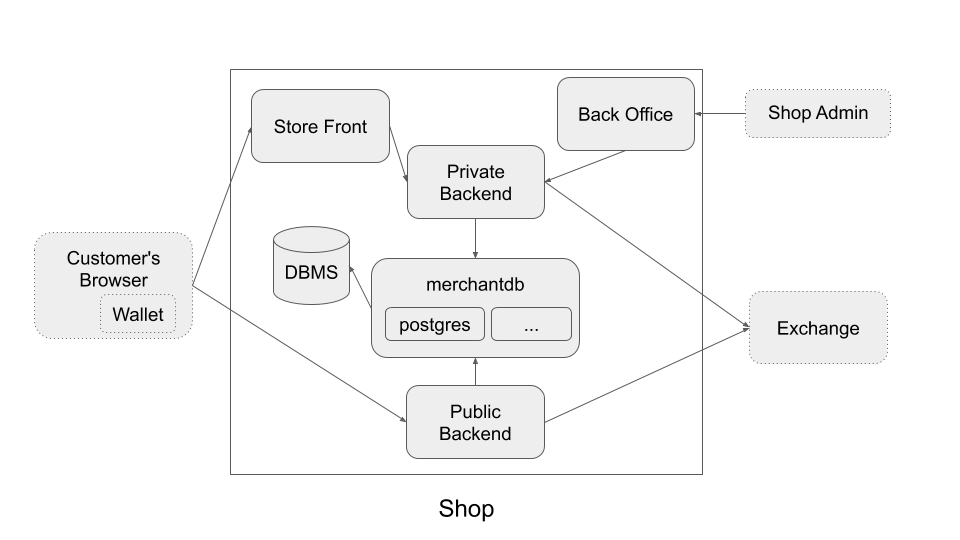
\includegraphics[width=\textwidth]{diagrams/taler-diagram-merchant.png}
    \caption{Architecture of the merchant reference implementation}
\end{figure}

The Taler merchant backend is a component that abstracts away the details of
processing Taler payments and provides a simple HTTP API.  The merchant backend
handles cryptographic operations (signature verification, signing), secret
management and communication with the exchange.

The backend API\footnote{See \url{https://docs.taler.net/api/} for the full documentation}
is divided into two types of HTTP endpoints:
\begin{enumerate}
  \item Functionality that is accessed internally by the merchant.  These APIs typically
    require authentication and/or are only accessible from within the private
    network of the merchant.
  \item Functionality that is exposed publicly on the Internet and accessed by the customer's wallet and browser.
    % FIXME: talk about proxying
\end{enumerate}

A typical merchant has a \emph{storefront} component that customers visit with
their browser, as well as a \emph{back office} component that allows the
merchant to view information about payments that customers made and that integrates
with other components such as order processing and shipping.

\subsection{Processing payments}\label{sec:processing-payments}

To process a payment, the storefront first instructs the backend to create an
\emph{order}.  The order contains information relevant to the purchase, and is
in fact a subset of the information contained in the contract terms.  The
backend automatically adds missing information to the order details provided by
the storefront.  The full contract terms can only be signed once the customer
provides the claim public key for the contract.

Each order is uniquely identified by an order ID, which can be chosen by the
storefront or automatically generated by the backend.

The order ID can be used to query the status of the payment.  If the customer
did not pay for an order ID yet, the response from the backend includes a
payment redirect URL.  The storefront can redirect the customer to this
payment redirect URL; visiting the URL will trigger the customer's
browser/wallet to prompt for a payment.

To simplify the implementation of the storefront, the merchant backend can
serve a page to the customer's browser that triggers the payment via the HTTP
402 status code and the corresponding headers, and provides a fallback (in the
form of a \texttt{taler:pay} link) for loosely integrated browsers.
When checking the status of a payment that is not settled yet, the response from the merchant backend
will contains a payment redirect URL.  The storefront redirects the browser to this URL,
which is served by the merchant backend and triggers the payment.

The code snippet shown in Figure~\ref{fig:merchant-donations-code} implements
the core functionality of a merchant frontend that prompts the customer for a
donation (upon visiting \texttt{/donate} with the right query parameters) and
shows a donation receipt on the fulfillment page with URL \texttt{/receipt}.
The code snippet is written in Python and uses the Flask library\footnote{\url{http://flask.pocoo.org/}} to process HTTP requests.
The helper functions \texttt{backend\_post}
and \texttt{backend\_get} make an HTTP \texttt{POST}/\texttt{GET} request to the merchant backend, respectively,
with the given request body / query parameters.

\begin{figure}
\lstinputlisting[language=Python,basicstyle=\footnotesize]{snippets/donations.py}
\caption[Code snippet for merchant frontend]{Code snippet with core functionality of a merchant frontend to accept donations.}
\label{fig:merchant-donations-code}
\end{figure}


\subsection{Back Office APIs}

The back office API allows the merchant to query information about the history
and status of payments, as well as correlate wire transfers to the merchant's
bank account with the respective GNU Taler payment.  This API is necessary to
allow integration with other parts of the merchant's e-commerce infrastructure.

%\subsection{Instances}
%Merchant instances allow one deployment of the merchant backend to host more
%than one logical merchant.  

\subsection{Example Merchant Frontends}

We implemented the following applications using the merchant backend API.

\begin{description}
  \item[Blog Merchant] The blog merchant's landing page has a list of article titles with a teaser.
    When following the link to the article, the customer is asked to pay to view the article.
  \item[Donations]  The donations frontend allows the customer to select a project to donate to.
    The fulfillment page shows a donation receipt.
  \item[Codeless Payments]  The codeless payment frontend is a prototype for a
    user interface that allows merchants to sell products on their website
    without having to write code to integrate with the merchant backend.
    Instead, the merchant uses a web interface to manage products and their
    available stock.  The codeless payment frontend then creates an HTML snippet with a payment
    button that the merchant can copy-and-paste integrate into their storefront.
  \item[Survey]  The survey frontend showcases the tipping functionality of GNU Taler.
    The user fills out a survey and receives a tip for completing it.
  \item[Back office] The example back-office application shows the history and
    status of payments processed by the merchant.
\end{description}

The code for these examples is available at \url{https://git.taler.net/} in the
repositories \texttt{blog}, \texttt{donations}, \texttt{codeless}, \texttt{survey}
and \texttt{backoffice} respectively.


\section{Wallet}

\begin{figure}
    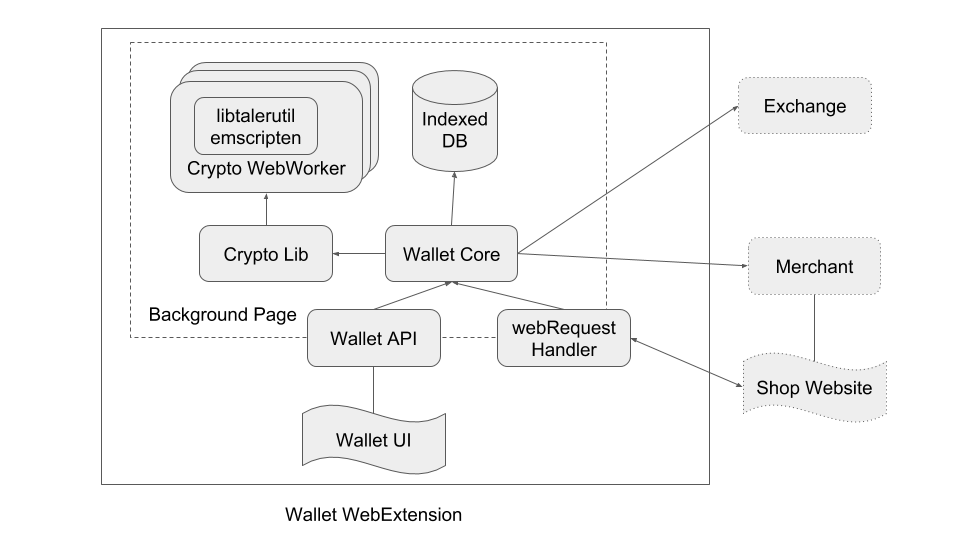
\includegraphics[width=\textwidth]{diagrams/taler-diagram-wallet.png}
    \caption{Architecture of the wallet reference implementation}
\end{figure}

The wallet manages the customer's reserves and coins, lets the customer view
and pay for contracts from merchants.  It can be seen in operation in
Section~\ref{sec:intro:ux}.

The reference implementation of the GNU Taler wallet is written in the
TypeScript language against the WebExtension API%
\footnote{\url{https://developer.mozilla.org/en-US/docs/Mozilla/Add-ons/WebExtensions}}, a cross-browser mechanism for
browser extensions.  The reference wallet is a ``tightly integrated'' wallet, as it directly hooks into
the browser to process responses with the HTTP status code ``402 Payment Required''.

Many cryptographic operations needed to implement the wallet are not commonly
available in a browser environment.  We cross-compile the GNU Taler utility
library written in C as well as its dependencies (such as libgcrypt) to asm.js
(and WebAssembly on supported platforms) using the LLVM-based emscripten
toolchain \cite{zakai2011emscripten}.

Cryptographic operations run in an isolated process implemented as a
WebWorker.\footnote{\url{https://html.spec.whatwg.org/}}  This design allows
the relatively slow cryptographic operations to run concurrently in the
background in multiple threads.  Since the crypto WebWorkers are started on-demand,
the wallet only uses minimal resources when not actively used.

\subsection{Optimizations}\label{sec:wallet-optimizations}
To improve the perceived performance of cryptographic operations,
the wallet optimistically creates signatures in the background
while the user is looking at the ``confirm payment'' dialog.  If the user does
not accept the contract, these signatures are thrown away instead of being sent
to the merchant.  This effectively hides the latency of the
most expensive cryptographic operations, as they are done while the user
consciously needs to make a decision on whether to proceed with a payment.


\subsection{Coin Selection}
The wallet hides the implementation details of fractionally spending different
denomination from the user, and automatically selects which denominations to
use for withdrawing a given amount, as well as which existing coins to
(partially) spend for a payment.

Denominations for withdrawal are greedily selected, starting with the largest
denomination that fits into the remaining amount to withdraw.  Coin selection
for spending proceeds similarly, but first checks if there is a single coin
that can be partially spent to cover the whole amount.  After each payment, the
wallet automatically refreshes coins with a remaining amount large enough to be
refreshed.  We discuss a simple simulation of the current coin selection algorithm
in Section~\ref{sec:coins-per-transaction}.

A more advanced coin selection would also consider the fee structure of the
exchange, minimizing the number of coins as well as the fees incurred by the
various operations.  The wallet could additionally learn typical amounts that
the user spends, and adjust withdrawn denominations accordingly to further
minimize costs.  An opposing concern to the financial cost is the anonymity of
customers, which is improved when the spending behavior of wallets is as
similar as possible.

% FIXME: what about anonymity effects of coin selection?

\subsection{Wallet Detection}
When websites such as merchants or banks try to signal the Taler wallet---for example,
to request a payment or trigger reserve creation---it is possible that the
customer simply has no Taler wallet installed.  To accommodate for this situation in a
user-friendly way, the HTTP response containing signaling to wallet should
contain as response body an HTML page with (1) a \texttt{taler:} link to
manually open loosely integrated wallets and (2) instructions on how to install
a Taler wallet if the user does not already have one.

It might seem useful to dynamically update page content depending on whether
the Taler wallet is installed, for example, to hide or show a ``Pay with Taler''
or ``Withdraw to Taler wallet'' option.  This functionality cannot be provided
in general, as only the definitive presence of a wallet can be detected, but
not its absence when the wallet is only loosely integrated in the user's
browser via a handler for the \texttt{taler:} URI scheme.

We nevertheless consider the ability to know whether a customer has definitely
installed a Taler wallet useful (if only for the user to confirm that the
installation was successful), and expose two APIs to query this.  The first one
is JavaScript-based and allows to register a callback for the when
presence/absence of the wallet is detected.  The second method works without
any JavaScript on the merchant's page, and uses CSS~\cite{sheets1998level} to dynamically show/hide
element on the page marked with the special \texttt{taler-installed-show} and
\texttt{taler-installed-hide} CSS classes, whose visibility is changed when
a wallet browser extension is loaded.

Browser fingerprinting \cite{mulazzani2013fast} is a concern with any
additional APIs made available to websites, either by the browser itself or by
browser extensions.  Since a website can simply try to trigger a payment to
determine whether a tightly integrated Taler wallet is installed, one bit of
additional fingerprinting information is already available through the usage of
Taler.  The dynamic detection methods do not, however, expose any information
that is not already available to websites by signaling the wallet through HTTP
headers.

\subsection{Backup and Synchronization}
While users can manually import and export the state of the wallet, at the time
of writing this, automatic backup and synchronization between wallets is not
implemented yet.  We discuss the challenges with implementing backup and
synchronization in a privacy-preserving manner in
Chapter~\ref{sec:future-work-backup-sync}.


\subsection{Wallet Liquidation}
If a customer wishes to stop using GNU Taler, they can deposit the remaining
coins in their wallet back to their own bank account.  We call this process
\emph{liquidation}.

In deployments with relatively lenient KYC regulation, the normal deposit
functionality used by merchants is used for wallet liquidation.  The wallet
simply acts as a merchant for one transaction, and asks the exchange to deposit
the coins into the customer's bank account.

However in deployments with strict KYC regulations, the customer would first
have to register and complete a KYC registration procedure with the exchange.
To avoid this, liquidation can be implemented as a modified deposit, which
restricts the payment to the bank account that was used to create a reserve of
the customer.

The exchange cannot verify that a coin that is being liquidated actually
originated the reserve that the customer claims it originated from, unless the
user reveals the protocol transcripts for withdrawal and refresh operations on
that coin, violating their privacy.  Instead, each reserve tracks the amount
that was liquidated into it, and the exchange rejects a liquidation request if
the liquidated amount exceeds the amount that was put into the reserve.  Note
that liquidation does not refill the funds of a reserve, but instead triggers a
bank transfer of the liquidated amount to the bank account that
created the reserve.


\subsection{Wallet Signaling}
We now define more precisely the algorithm that the wallet executes when a
website signals to that wallet that an operation related to payments should be
triggered, either by opening a \texttt{taler:pay} URL or by responding
with HTTP 402 and at least one Taler-specific header.

% FIXME:  need to specify what happens when gateway_origin="", for example when triggered
% via URL
The steps to process a payment trigger are as follows.  The algorithm takes the
following parameters: \texttt{current\_url} (the URL of the page that
raises the 402 status or \texttt{null} if triggered by a \texttt{taler:pay} URL),
\texttt{contract\_url}, \texttt{resource\_url}, \texttt{session\_id},
\texttt{offer\_url}, \texttt{refund\_url}, \texttt{tip\_token} (from the
``Taler-\dots'' headers or \emph{taler:pay} URL parameters respectively)
\begin{enumerate}
  \item If \texttt{resource\_url} a non-empty string, set \texttt{target\_url} to \texttt{resource\_url},
    otherwise set \texttt{target\_url} to \texttt{current\_url}.
  \item If \texttt{target\_url} is empty, stop.
  \item If there is an existing payment $p$ whose
    fulfillment URL equals \texttt{target\_url} and either \texttt{current\_url} is \texttt{null}
    or \texttt{current\_url} has the same origin as
    either the fulfillment URL or payment URL in the contract terms, then:
    \begin{enumerate}[label*=\arabic*.]
      \item If \texttt{session\_id} is non-empty and the last session ID for payment $p$ was recorded
        in the wallet with session signature $sig$, construct a fulfillment instance URL from $sig$ 
        and the order ID of $p$.
      \item Otherwise, construct an extended fulfillment URL from the order ID of $p$.
      \item Navigate to the extended fulfillment URL constructed in the previous step and stop.
    \end{enumerate}
  \item If \texttt{contract\_url} is a non-empty URL, execute the steps for
    processing a contract URL (with \texttt{session\_id}) and stop.
  \item If \texttt{offer\_url} is a non-empty URL, navigate to it and stop.
  \item If \texttt{refund\_url} is a non-empty URL, process the refund and stop.
  \item If \texttt{tip\_url} is a non-empty URL, process the tip and stop.
\end{enumerate}

For interactive web applications that request payments, such as games or single
page apps (SPAs), the payments initiated by navigating to a page with HTTP
status code 402 are not appropriate, since the state of the web application is
destroyed by the navigation.  Instead the wallet can offer a JavaScript-based
API, exposed as a single function with a subset of the parameters of the
402-based payment: \texttt{contract\_url}, \texttt{resource\_url},
\texttt{session\_id} \texttt{refund\_url}, \texttt{offer\_url},
\texttt{tip\_token}.  Instead of navigating away, the result of the operation
is returned as a JavaScript promise (either a payment receipt, refund
confirmation, tip success status or error).  If user input is required (e.g., to
ask for a confirmation for a payment), the page's status must not be destroyed.
Instead, an overlay or separate tab/window displays the prompt to the user.
% FIXME:  should be specify the full algorithm for JS payments?

% FIXME talk about clickjacking



\newcommand\inecc{\in \mathbb{Z}_{|\mathbb{E}|}}
\newcommand\inept{\in {\mathbb{E}}}
\newcommand\inrsa{\in \mathbb{Z}_{|\mathrm{dom}(\FDH_K)|}}

\section{Cryptographic Protocols}

\def\HKDF{\textrm{HKDF}}
\def\KDF{\textrm{KDF}}
\def\FDH{\textrm{FDH}}
\newcommand{\iseq}{\stackrel{?}{=}}
\newcommand{\iseqv}{\stackrel{?}{\equiv}}
\newcommand{\pccheck}{\mathbf{check}\ }

In this section, we describe the main cryptographic protocols for Taler in more
detail.  The more abstract, high-level protocols from
Section~\ref{sec:crypto:instantiation} are instantiated and and embedded in
concrete protocol diagrams that can hopefully serve as a reference for
implementors.

For ease of presentation, we do not provide a bit-level description of the
cryptographic protocol.  Some details from the implementation are left out,
such as fees, additional timestamps in messages and checks for the expiration
of denominations. Furthermore, we do not specify the exact responses in the
error cases, which in the actual implementation should include signatures that
could be used during a legal dispute.  Similarly, the actual implementation
contains some additional signatures on messages sent that allow to prove to a
third party that a participant did not follow the protocol.

As we are dealing with financial transactions, we explicitly describe whenever
entities need to safely write data to persistent storage.  As long as the data
persists, the protocol can be safely resumed at any step.  Persisting data is
cumulative, that is an additional persist operation does not erase the
previously stored information.

The implementation also records additional entries in the exchange's database
that are needed for auditing.

\subsection{Preliminaries}
In our protocol definitions, we write $\mathbf{check}\ \mathrm{COND}$ to abort
the protocol with an error if the condition $\mathrm{COND}$ is false.

We use the following algorithms:
\begin{itemize}
\item $\algo{Ed25519.Keygen}() \mapsto \langle \V{sk}, \V{pk} \rangle$
    to generate an Ed25519 key pair.
 \item $\algo{Ed25519.GetPub}(\V{sk}) \mapsto \V{pk}$ to derive the public key from
    an Ed25519 public key.
 \item $\algo{Ed25519.Sign}(\V{sk}, m) \mapsto \sigma$ to create a signature $\sigma$
    on message $m$ using secret key $\V{sk}$.
 \item $\algo{Ed25519.Verify}(\V{pk}, \sigma, m) \mapsto b$ to check if $\sigma$ is
   a valid signature from $\V{pk}$ on message $m$.
 \item $\mathrm{HKDF}(n, k, s) \mapsto m$ is the HMAC-based key derivation function \cite{rfc5869},
   producing an output $m$ of $n$ bits from the input key material $k$ and salt $s$.
\end{itemize}

We write $\mathbb{Z}^*_N$ for the multiplicative group of integers modulo $N$.
Given an $r \in \mathbb{Z}^*_N$, we write $r^{-1}$ for the multiplicative
inverse modulo $N$ of $r$.

We write $H(m)$ for the SHA-512 hash of a bit string.

We write $\FDH(N,m)$ for the full domain hash that maps the bit string $m$ to
an element of $\mathbb{Z}^*_N$.  Specifically, $\FDH(N,m)$ is computed by
first computing $H(m)$. Let $b := \lceil \log_2 N\rceil$.  The full domain
hash is then computed by iteratively computing a HKDF to obtain $b$ bits of
output until the $b$-bit value is below $N$.  The inputs to the HKDF are a
``secret key'', a fixed context plus a 16-bit counter (in big endian) as a
context chunk that is incremented until the computation succeeds.  For the
source key material, we use a binary encoding of the public RSA key with
modulus $N$.\footnote{So technically, it is $\FDH(N,e,m)$, but we use the
  simplified notation $\FDH(N,m)$.}  Here, the public RSA key is encoded by
first expressing the number of bits of the modulus and the public exponent as
16-bit numbers in big endian, followed by the two numbers (again in unsigned
big endian encoding).\footnote{See
  \texttt{GNUNET\_CRYPTO\_rsa\_public\_key\_encode()}.}  For the context, the
C-string ``RSA-FDA FTpsW!'' (without 0-termination) is used.  For the KDF, we
instantiate the HKDF described in RFC 5869~\cite{rfc5869} using HMAC-SHA512 as
XTR and HMAC-SHA256 as PRF*.\footnote{As suggested in
  \url{http://eprint.iacr.org/2010/264.pdf}} Let the result of the first
successful iteration of the HKDF function be $r$ with $0 \le r < N$.  Then, to
protect against a malicious exchange when blinding values, the $FDH(N,m)$
function checks that $\gcd(r,n) = 1$. If not, the $\FDH(n,m)$ calculation
fails because $n$ is determined to be malicious.

The expression $x \randsel X$ denotes uniform random selection of an element
$x$ from set $X$.  We use $\algo{SelectSeeded}(s, X) \mapsto x$ for pseudo-random uniform
selection of an element $x$ from set $X$ and seed $s$.  Here, the result is deterministic for fixed inputs $s$ and $X$.

The exchange's denomination signing key pairs $\{\langle \V{skD}_i, \V{pkD}_i \rangle \}$ are RSA keys pairs,
and thus $\V{pkD}_i = \langle e_i, N_i \rangle$, $\V{skD_i} = d_i$.  We write $D(\V{pkD}_i)$ for the
financial value of the denomination $\V{pkD}_i$.

% FIXME: explain RSA keys of exchange


\subsection{Withdrawing}
The withdrawal protocol is defined in Figure~\ref{fig:withdraw-protocol}.
The following additional algorithms are used, which we only define informally here:
\begin{itemize}
  \item $\algo{CreateBalance}(W_p, v) \mapsto \bot$ is used by the exchange,
    and has the side-effect of creating a reserve record with balance $v$
    and reserve public key (effectively the identifier of the reserve) $W_p$.
  \item $\algo{GetWithdrawR}(\rho) \mapsto \{\bot,\overline{\sigma}_C\}$
    is used by the exchange, and checks
    if there is an existing withdraw request $\rho$.  If the existing request
    exists, the existing blind signature $\overline{\sigma}_C$ over
    coin $C$ is returned.  On a fresh request, $\bot$ is
    returned.
  \item $\algo{BalanceSufficient}(W_s,\V{pkD}_t) \mapsto b$ is used by the exchange, and
    returns true if the balance in the reserve identified by $W_s$ is sufficient to
    withdraw at least one coin if denomination $\V{pkD}_t$.
  \item $\algo{DecreaseBalance}(W_s,\V{pkD}_t) \mapsto \bot$ is used by the exchange, and
    decreases the amount left in the reserve identified by $W_s$ by the amount $D(\V{pkD}_t)$
    that the denomination $\V{pkD}_t$ represents.
\end{itemize}

\begin{figure}
\centering
\fbox{%
\pseudocode[codesize=\small]{%
\textbf{Customer} \< \< \textbf{Exchange} \\
  \text{Knows } \{ \langle e_i,N_i \rangle \} = \{\V{pkD}_i\} \< \< \text{Knows } \{ \langle \V{skD}_i, \V{pkD}_i \rangle \} \pclb
\pcintertext[dotted]{Create Reserve} 
\langle w_s, W_p \rangle \leftarrow \algo{Ed25519.Keygen}() \< \< \\
\text{Persist reserve } \langle w_s,v \rangle \< \< \\
  \< \sendmessageright{top={Bank transfer}, bottom={(subject: $W_p$, amount: $v$)},style=dashed} \< \\
  \< \< \algo{CreateBalance}(W_p, v) \pclb
\pcintertext[dotted]{Prepare Withdraw}
\text{Choose $t$ with $\V{pkD}_t \in \{\V{pkD}_i\}$} \< \< \\
\langle c_s, C_p \rangle \leftarrow \algo{Ed25519.Keygen}() \< \< \\
  r \randsel \mathbb{Z}^*_N \< \< \\
  \text{Persist planchet } \langle c_s, r \rangle \< \< \pclb
\pcintertext[dotted]{Execute Withdraw}
\overline{m} := \FDH(N_t, C_p) \cdot r^{e_t} \bmod N_t \< \< \\
\rho_W := \langle \V{pkD}_t, \overline{m} \rangle \< \< \\
\sigma_W := \algo{Ed25519.Sign}(w_s, \rho_W) \< \< \\
\< \sendmessageright*{\rho := \langle W_p, \sigma_W, \rho_W \rangle} \< \\
  \< \< \pccheck \V{pkD}_t \in  \{ \V{pkD}_i \} \\
\< \< \pccheck \algo{Ed25519.Verify}(W_p,\rho_W,\sigma_W) \\
\< \< x \leftarrow \algo{GetWithdraw}(\rho) \\
\< \< \pcif x \iseq \bot \\
\< \< \t \pccheck \algo{BalanceSufficient}(W_p,\V{pkD}_t) \\
\< \< \t \algo{DecreaseBalance}(W_p, \V{pkD}_t) \\
\< \< \t \text{Persist withdrawal $\rho$} \\
\< \< \t \overline{\sigma}_C := (\overline{m})^{\V{skD}_t} \bmod N_t \\
\< \< \pcelse \\
\< \< \t \overline{\sigma}_C := x \\
\< \sendmessageleft*{\overline{\sigma}_C} \< \\
\sigma_C := r^{-1}\overline{\sigma}_C \< \< \\
\pccheck \sigma_C^{e_t} \iseqv_{N_t} \FDH(N_t, C_p) \< \< \\
\text{Persist coin $\langle \V{pkD}_t, c_s, C_p, \sigma_C \rangle$}  \< \< \\
}
}
\caption[Withdraw protocol diagram.]{Withdrawal protocol diagram.}
\label{fig:withdraw-protocol}
\end{figure}

\subsection{Payment transactions}
The payment protocol is defined in two parts.  First, the spend protocol in
Figure~\ref{fig:payment-spend} defines the interaction between a merchant and
a customer.  The customer obtains the contract terms (as $\rho_P$) from the
merchant, and sends the merchant deposit permissions as a payment.  The deposit protocol
in Figure~\ref{fig:payment-deposit} defines how subsequently the merchant sends the
deposit permissions to the exchange to detect double-spending and ultimately
to receive a bank transfer from the exchange.

Note that in practice the customer can also execute the deposit
protocol on behalf of the merchant. This is useful in situations where
the customer has network connectivity but the merchant does not. It
also allows the customer to complete a payment before the payment
deadline if a merchant unexpectedly becomes unresponsive, allowing the
customer to later prove that they paid on time.

We limit the description to one exchange here, but in practice, the merchant
communicates to the customer the exchanges that it supports, in addition to the
account information $A_M$ that might differ between exchanges.

We use the following algorithms, defined informally here:
\begin{itemize}
 \item $\algo{SelectPayCoins}(v, E_M) \mapsto \{ \langle \V{coin}_i, f_i \rangle \}$ selects
   fresh coins (signed with denomination keys from exchange $E_M$)
   to pay for the amount $v$.  The result is a set of coins
   together with the fraction of each coin that must be spent such that
   the amounts contributed by all coins sum up to $v$.
 \item $\algo{MarkDirty}(\V{coin}, f) \mapsto \bot$ subtracts the fraction $f$ from the
   available amount left on a coin, and marks the coin as dirty (to trigger refreshing
   in case $f$ is below the denomination value).  Thus, assuming the coin has
   any residual value, the customer's wallet will do a refresh on $\V{coin}$
   and not use it for further payments.  This provides unlinkability of transactions
   made with change arising from paying with fractions of a coin's denomination.
 \item $\algo{Deposit}(E_M, D_i) \mapsto b$ executes the second part of the payment protocol
   (i.e., the deposit) with exchange $E_M$, using deposit permission $D_i$.
 \item $\algo{GetDeposit}(C_p, h) \mapsto \{\bot,\rho_{(D,i)}\}$ checks in the exchange's database
    for an existing processed deposit permission on coin $C_p$ for the contract
    identified by $h$.  The algorithm returns the existing deposit permission $\rho_{(D,i)}$, or $\bot$ if a
    matching deposit permission is not recorded.
 \item $\algo{IsOverspending}(C_p, \V{pkD}, f) \mapsto b$ checks in the exchange's database
   if there if at least the fraction $f$ of the coin $C_p$ of denomination $\V{pkD}$ is still available
   for use, based on existing spend/withdraw records of the exchange.
 \item $\algo{MarkFractionalSpend}(C_p, f) \mapsto \bot$ adds a spending
   record to the exchanges database, indicating
   that fraction $f$ of coin $C_p$ has been spent (in addition to
   existing spending/refreshing records).
 \item $\algo{ScheduleBankTransfer}(A_M, f, \V{pkD}, h_c) \mapsto \bot$
   schedules a bank transfer from the exchange to
   the account identified by $A_M$, for subject $h_c$ and for the amount $f\cdot D(\V{pkD})$.
   % NOTE: actual implementation avoids multiplication (messy!) and would
   % simply require f \le D(\V{pkD})!
\end{itemize}


\begin{figure}
\centering
\fbox{%
\pseudocode[codesize=\footnotesize]{%
\textbf{Customer} \< \< \textbf{Merchant} \\
\text{Knows } \V{pkM} \< \< \text{Knows } \langle \V{pkM}, \V{skM} \rangle \\
\< \sendmessageright{top={Select product/service},style=dashed} \< \\
\< \< \text{Determine:} \\
\< \< \text{$\bullet$ } v \text{ (price) } \\
\< \< \text{$\bullet$ } E_M \text{ (exchange) } \\
\< \< \text{$\bullet$ } A_M \text{ (acct.) } \\
\< \< \text{$\bullet$ } \V{info} \text{ (free-form details) } \\
\< \sendmessageleft{top={Request payment},style=dashed} \< \\
\langle p_s, P_p \rangle \leftarrow \algo{Ed25519.Keygen}() \< \< \\
\text{Persist ownership identifier } p_s \< \< \\
\< \sendmessageright*{P_p} \< \\
  \< \< \rho_P := \langle E_M, A_M, \V{pkM}, H(\langle v, \V{info}\rangle), P_p \rangle \\
\< \< \sigma_P := \V{Ed25519.Sign}(\V{skM}, \rho_P) \\
\< \sendmessageleft*{\rho_P, \sigma_P, v, \V{info}} \< \\
  \langle M, A_M, \V{pkM}, h', P_p' \rangle := \rho_P \< \< \\
\pccheck \algo{Ed25519.Verify}(pkM, \sigma_P, \rho_P) \< \< \\
\pccheck P_p' \iseq P_p \< \< \\
\pccheck h' \iseq H(\langle v, \V{info} \rangle ) \< \< \\
\V{cf} \leftarrow \algo{SelectPayCoins}(v, E_M) \< \< \\
\pcfor \langle \V{coin_i,f_i} \rangle \in \V{cf} \< \< \\
\t \algo{MarkDirty}(\V{coin}_i, f_i) \< \< \\
\t \langle c_s, C_p, \V{pkD}, \sigma_C \rangle := \V{coin}_i \< \< \\
  \t \rho_{(D,i)} := \langle C_p, \V{pkD}, \sigma_C, f_i, H(\rho_P), A_M, \V{pkM} \rangle \< \< \\
\t \sigma_{(D,i)} := \V{Ed25519.Sign}(c_s, \rho_{(D,i)}) \< \< \\
  \text{Persist } \langle \sigma_P, \V{cf}, \rho_P, \rho_{(D,i)}, \sigma_{(D,i)}, v, \V{info} \rangle \< \<\\
\< \sendmessageright*{ \mathcal{D} := \{\langle \rho_{(D,i)}, \sigma_{(D,i)}\rangle \}} \< \\
\< \< \pcfor D_i \in \mathcal{D} \\
\< \< \t \pccheck \algo{Deposit}(E_M, D_i) \\
}
}
\caption[Spend protocol diagram.]{Spend Protocol executed between customer and merchant for the purchase
  of an article of price $v$ using coins from exchange $E_M$. The merchant has
  provided his account details to the exchange under an identifier $A_M$.
  The customer can identify themselves as the one who received the offer
  using $p_s$.
  %This prevents multiple customers from legitimately paying for the
  %same article and potentially exhausting stocks.
}
\label{fig:payment-spend}
\end{figure}

\begin{figure}
\centering
\fbox{%
\pseudocode[codesize=\small]{%
\textbf{Customer/Merchant} \< \< \textbf{Exchange} \\
\text{Knows } \V{pkESig} \< \< \text{Knows } \V{skESig}, \V{pkESig}, \{ \V{pkD}_i \} \\
\text{Knows } D_i = \langle \rho_{(D,i)}, \sigma_{(D,i)} \rangle \< \< \\
\< \sendmessageright*{ D_i } \< \\
\< \< \langle \rho_{(D,i)}, \sigma_{(D,i)} \rangle := D_i \\
  \< \< \langle C_p, \V{pkD}, \sigma_C, f_i, h, A_M, \V{pkM} \rangle := \rho_{(D,i)} \\
\< \< \pccheck \V{pkD} \in \{ \V{pkD}_i \} \\
\< \< \langle e, N \rangle := \V{pkD} \\
\< \< \pccheck \algo{Ed25519.Verify}(C_p, \sigma_{(D,i)}, \rho_{(D,i)}) \\
\< \< x \leftarrow \algo{GetDeposit}(C_p, h) \\
\< \< \pcif x \iseq \bot  \\
\< \< \t \pccheck \sigma_C^{e} \iseqv_N \FDH(N, C_p) \\
\< \< \t \pccheck \neg\algo{IsOverspending}(C_p, \V{pkD}, f) \\
\< \< \t \text{Persist deposit-record } D_i \\
\< \< \t \algo{MarkFractionalSpend}(C_p, f) \\
\< \< \t \algo{ScheduleBankTransfer}(A_M, f, \V{pkD}, h_c) \\
\< \< \pcelse \\
\< \< \t \pccheck x \iseq \rho_{(D,i)} \\
\< \< \sigma_{DC} \leftarrow \algo{Ed25519.Sign}(\V{pkESig}, \rho_{(D,i)}) \\
\< \sendmessageleft*{ \sigma_{DC} } \< \\
\pccheck \algo{Ed25519.Verify} \\{}\qquad(\V{pkESig}, \sigma_{DC}, \rho_{(D,i)}) \< \< \\
}
}
\caption[Deposit protocol diagram.]{Deposit Protocol run for each deposited coin $D_i \in {\cal D}$ with the
  exchange that signed the coin.}
\label{fig:payment-deposit}
\end{figure}


\subsection{Refreshing and Linking}
The refresh protocol is defined in Figures~\ref{fig:refresh-part1} and
\ref{fig:refresh-part2}.  The refresh protocol allows the customer to
obtain change for the remaining fraction of the value of a coin.  The
change is generated as a fresh coin that is unlinkable to the dirty
coin to anyone except for the owner of the dirty coin.

A na\"ive implementation of a refresh protocol that just gives the customer a
new coin could be used for peer-to-peer transactions that hides income from tax
authorities.  Thus, (with probability $(1-1/\kappa)$) the refresh protocol
records information that allows the owner of the original coin to obtain the
refreshed coin from the original coin via the linking protocol (illustrated in
Figure~\ref{fig:link}).

We use the following algorithms, defined informally here:
\begin{itemize}
  \item \algo{RefreshDerive} is defined in Figure~\ref{fig:refresh-derive}.
  \item $\algo{GetOldRefresh}(\rho_{RC}) \mapsto \{\bot,\gamma\}$ returns the past
    choice of $\gamma$ if $\rho_{RC}$ is a refresh commit message that has been seen before,
    and $\bot$ otherwise.
  \item $\algo{IsConsistentChallenge}(\rho_{RC}, \gamma) \mapsto \{ \bot,\top \}$ returns
    $\top$ if no refresh-challenge has been persisted for the refresh operation by commitment
    $\rho_{RC}$ or $\gamma$ is consistent with the persisted (and thus previously received) challenge;
    returns $\bot$ otherwise.
  \item $\algo{LookupLink}(C_p) \mapsto \{ \langle \rho_{L}^{(i)}, \sigma_L^{(i)},
  \overline{\sigma}_C^{(i)} \rangle \}$ looks up refresh records on coin with public key $C_p$ in
    the exchange's database and returns the linking message $\rho_L^{(i)}$, linking
    signature $\sigma_L^{(i)}$ and blinded signature $\overline{\sigma}_C^{(i)}$ for each refresh
    record $i$.
\end{itemize}


\begin{figure}
\centering
\fbox{%
\procedure[codesize=\small]{$\algo{RefreshDerive}(s, \langle e, N \rangle, C_p)$}{%
t := \HKDF(256, s, \texttt{"t"}) \\
T := \algo{Curve25519.GetPub}(t) \\
x := \textrm{ECDH-EC}(t, C_p)  \\
r := \algo{SelectSeeded}(x, \mathbb{Z}^*_{N})  \\
c_s := \HKDF(256, x, \texttt{"c"}) \\
C_p := \algo{Ed25519.GetPub}(c_s)  \\
\overline{m} := r^{e}\cdot C_p \mod N \\
\pcreturn \langle t, T, x, c_s, C_p, \overline{m} \rangle
}
}
\caption[RefreshDerive algorithm]{The RefreshDerive algorithm running with the seed $s$ on dirty coin $C_p$ to
   generate a fresh coin to be later signed with denomination key $pkD := \langle e,N\rangle$.}
\label{fig:refresh-derive}
\end{figure}


\begin{figure}
\centerline{
\fbox{%
\pseudocode[codesize=\footnotesize]{%
\textbf{Customer} \< \< \textbf{Exchange} \\
\text{Knows } \{ \V{pkD}_i \} \< \< \text{Knows } \{\langle  \V{skD}_i, \V{pkD}_i \rangle \}  \\
\text{Knows } \V{coin}_0 = \langle \V{pkD}_0, c_s^{(0)}, C_p^{(0)}, \sigma_{C}^{(0)} \rangle \< \<  \\
\text{Select } \langle N_t, e_t \rangle := \V{pkD}_t \in \{ \V{pkD}_i \} \< \<  \\
\pcfor i = 1,\dots,\kappa \< \<  \\
\t s_i \randsel \{0,1\}^{256} \< \<  \\
\t X_i := \algo{RefreshDerive}(s_i, \V{pkD}_t, C_p^{(0)}) \< \< \\
\t (t_i, T_i, x_i, c_s^{(i)}, C_p^{(i)}, \overline{m}_i) := X_i \< \< \\
h_T := H(T_1,\dots,T_\kappa)  \< \< \\
h_{\overline{m}} := H(\overline{m}_1,\dots,\overline{m}_\kappa) \< \< \\
h_C := H(h_t, h_{\overline{m}})  \< \< \\
\rho_{RC} := \langle h_C, \V{pkD}_t, \V{pkD}_0, C_p^{(0)}, \sigma_{C}^{(0)} \rangle \< \< \\
\sigma_{RC} := \algo{Ed25519.Sign}(c_s^{(0)}, \rho_{RC}) \< \< \\
\text{Persist refresh-request } \langle \rho_{RC}, \sigma_{RC} \rangle \< \< \\
\< \sendmessageright*{ \rho_{RC}, \sigma_{RC} }  \< \\
\< \<  (h_C, \V{pkD}_t, \V{pkD}_0, C_p^{(0)}, \sigma_{C}^{(0)}) := \rho_{RC} \\
\< \< \pccheck \algo{Ed25519.Verify}(C_p^{(0)}, \sigma_{RC}, \rho_{RC}) \\
\< \< x \leftarrow \algo{GetOldRefresh}(\rho_{RC}) \\
\< \< \pcif x \iseq \bot \\
\< \< \t v := D(\V{pkD}_t) \\
\< \< \t \langle e_0, N_0 \rangle := \V{pkD}_0 \\
\< \< \t \pccheck \neg\algo{IsOverspending}(C_p^{(0)}, \V{pkD}_0, v) \\
\< \< \t \pccheck \V{pkD}_t \in \{ \V{pkD}_i \} \\
\< \< \t \pccheck \FDH(N_0, C_p^{(0)}) \iseqv_{N_0} (\sigma_0^{(0)})^{e_0} \\
\< \< \t \algo{MarkFractionalSpend}(C_p^{(0)}, v) \\
\< \< \t \gamma \randsel \{1,\dots,\kappa\} \\
\< \< \t \text{Persist refresh-record } \langle \rho_{RC},\gamma \rangle \\
\< \< \pcelse \\
\< \< \t \gamma := x \\
\< \sendmessageleft*{ \gamma } \< \pclb
\pcintertext[dotted]{(Continued in Figure~\ref{fig:refresh-part2})}
}}}
\caption{Refresh Protocol (Commit Phase)}
\label{fig:refresh-part1}
\end{figure}

\begin{figure}
\centerline{
\fbox{%
\pseudocode[codesize=\footnotesize]{%
\textbf{Customer} \< \< \textbf{Exchange} \pclb
\pcintertext[dotted]{(Continuation of \ref{fig:refresh-part1})} \\
\< \sendmessageleft*{ \gamma } \< \\
\pccheck \algo{IsConsistentChallenge}(\rho_{RC}, \gamma) \< \< \\
\text{Persist refresh-challenge $\langle \rho_{RC}, \gamma  \rangle$}  \< \< \\
S := \langle s_1,\dots,s_{\gamma-1},s_{\gamma+1},\dots,s_\kappa \rangle \< \< \\
\rho_{L} = \langle C_p^{(0)}, \V{pkD}_t, T_\gamma, \overline{m}_\gamma \rangle \< \< \\
\rho_{RR} = \langle T_\gamma, \overline{m}_\gamma, S \rangle \< \< \\
\sigma_{L} = \algo{Ed25519.Sign}(c_s^{(0)}, \rho_{L}) \< \< \\ 
\< \sendmessageright*{ \rho_{RR}, \rho_{L}, \sigma_{L} } \< \\
\< \< \langle T'_\gamma, \overline{m}'_\gamma, S \rangle := \rho_{RR} \\
\< \< \langle s_1,\dots,s_{\gamma-1},s_{\gamma+1},\dots,s_\kappa \rangle ) := S \\
\< \< \pccheck \algo{Ed25519.Verify}(C_p^{(0)}, \sigma_L, \rho_L) \\
\< \< \pcfor i = 1,\dots,\gamma-1,\gamma+1,\dots,\kappa \\
\< \< \t X_i := \algo{RefreshDerive}(s_i, \V{pkD}_t, C_p^{(0)}) \\
\< \< \t \langle t_i, T_i, x_i, c_s^{(i)}, C_p^{(i)}, \overline{m}_i \rangle := X_i \\
\< \< h_T' = H(T_1,\dots,T_{\gamma-1},T'_{\gamma},T_{\gamma+1},\dots,T_\kappa) \\
\< \< h_{\overline{m}}' = H(\overline{m}_1,\dots,\overline{m}_{\gamma-1},\overline{m}'_{\gamma},\overline{m}_{\gamma+1},\dots,\overline{m}_\kappa) \\
\< \< h_C' = H(h_T', h_{\overline{m}}') \\
\< \< \pccheck h_C \iseq h_C' \\
\< \< \overline{\sigma}_C^{(\gamma)} := \overline{m}^{skD_t} \\
\< \sendmessageleft*{\overline{\sigma}_C^{(\gamma)}} \< \\
\sigma_C^{(\gamma)} := r^{-1}\overline{\sigma}_C^{(\gamma)} \< \< \\
\pccheck (\sigma_C^{(\gamma)})^{e_t} \iseqv_{N_t} C_p^{(\gamma)} \< \< \\
\text{Persist coin $\langle \V{pkD}_t, c_s^{(\gamma)}, C_p^{(\gamma)}, \sigma_C^{(\gamma)} \rangle$}  \< \< \\
}}}
\caption{Refresh Protocol (Reveal Phase)}
\label{fig:refresh-part2}
\end{figure}

\begin{figure}
\centering
\fbox{%
\pseudocode[codesize=\footnotesize]{%
\textbf{Customer} \< \< \textbf{Exchange} \\
\text{Knows } \V{coin}_0 = \langle \V{pkD}_0, c_s^{(0)}, C_p^{(0)}, \sigma_{C}^{(0)} \rangle \< \<  \\
\< \sendmessageright*{C_p^{(0)}} \< \\
\< \< L := \algo{LookupLink}(C_p^{(0)}) \\
\< \sendmessageleft*{L} \< \\
\pcfor \langle \rho_{L}^{(i)}, \overline{\sigma}_L^{(i)}, \sigma_C^{(i)} \rangle \in L \< \< \\
\t \langle \hat{C}_p^{(i)}, \V{pkD}_t^{(i)}, T_\gamma^{(i)}, \overline{m}_\gamma^{(i)} \rangle := \rho_L^{(i)} \< \< \\
\t \langle e_t^{(i)}, N_t^{(i)} \rangle := \V{pkD}_t^{(i)} \< \< \\
\t \pccheck \hat{C}_p^{(i)} \iseq  C_p^{(0)} \< \< \\
\t \pccheck \algo{Ed25519.Verify}(C_p^{(0)}, \rho_{L}^{(i)}, \sigma_L^{(i)})\< \< \\
\t x_i := \algo{ECDH}(c_s^{(0)}, T_\gamma^{(i)}) \< \< \\
\t r_i := \algo{SelectSeeded}(x_i, \mathbb{Z}^*_{N_t})  \\
\t c_s^{(i)} := \HKDF(256, x_i, \texttt{"c"}) \\
\t C_p^{(i)} := \algo{Ed25519.GetPub}(c_s^{(i)})  \\
\t \sigma_C^{(i)} := (r_i)^{-1} \cdot \overline{m}_\gamma^{(i)} \\
\t \pccheck (\sigma_C^{(i)})^{e_t^{(i)}} \iseqv_{N_t^{(i)}} C_p^{(i)} \\
\t \text{(Re-)obtain coin } \langle \V{pkD}_t^{(i)}, c_s^{(i)}, C_p^{(i)}, \sigma_C^{(i)} \rangle
}
}
\caption{Linking protocol}
\label{fig:link}
\end{figure}

\clearpage

\subsection{Refunds}
The refund protocol is defined in Figure~\ref{fig:refund}.  The customer
requests from the merchant that a deposit should be ``reversed'', and if the
merchants allows the refund, it authorizes the exchange to apply the refund and
sends the refund confirmation back to the customer.  Note that in practice,
refunds are only possible before the refund deadline, which is not considered
here.

We use the following algorithms, defined informally here:
\begin{itemize}
 \item $\algo{ShouldRefund}(\rho_P, m) \mapsto \{ \top, \bot \}$ is used by the merchant to
   check whether a refund with reason $m$ should be given for the purchase identified by the
    contract terms $\rho_P$.  The decision is made according to the merchant's business rules.
  \item $\algo{LookupDeposits}(\rho_P, m) \mapsto \{ \langle \rho_{(D,i)},
    \sigma_{(D,i)} \rangle \}$ is used by the merchant to retrieve deposit
    permissions that were previously sent by the customer and already deposited
    with the exchange.
  \item $\algo{RefundDeposit}(C_p, h, f, \V{pkM})$ is used by the exchange to
    modify its database.  It (partially) reverses the amount $f$ of a deposit
    of coin $C_p$ to the merchant $\V{pkM}$ for the contract identified by $h$.
    The procedure is idempotent, and subsequent invocations with a larger $f$
    increase the refund.
\end{itemize}

\begin{figure}
\centerline{
\fbox{%
\pseudocode[codesize=\footnotesize]{%
\< \< \pclb
\pcintertext[dotted]{Request refund} \\
\textbf{Customer} \< \< \textbf{Merchant} \\
\text{Knows } \V{pkM}, \V{pkESig} \< \< \text{Knows } \langle \V{pkM}, \V{skM} \rangle, \V{pkESig} \\
\< \sendmessageright{top={Ask for refund},bottom={(Payment $\rho_P$, reason $m$)},style=dashed} \< \\
\< \< \pccheck \algo{ShouldRefund}(\rho_P,m) \pclb
\pcintertext[dotted]{Execute refund} \\
\textbf{Exchange} \< \< \textbf{Merchant} \\
\text{Knows } \langle \V{skESig}, \V{pkESig} \rangle \< \<  \\
  \< \< \pcfor \langle \rho_{(D,i)}, \cdot  \rangle \in \algo{LookupDeposits}(\rho_P) \\
  \< \< \t \rho_{(X,i)} := \langle \mathtt{"refund"}, \rho_D \rangle \\
  \< \< \t \sigma_{(X,i)} :=  \algo{Ed25519.Sign}(\V{skM}, \rho_{(X,i)}) \\
  \< \sendmessageleft*{X := \{ \rho_{(X,i)}, \sigma_{(X,i)} \} } \< \\
\pcfor \langle \rho_{(X,i)}, \sigma_{(X,i)}  \rangle \in X \< \< \\
\t \pccheck \langle \mathtt{"refund"}, \rho_D \rangle := \rho_X \< \< \\
\t \pccheck \langle C_p, \V{pkD}, \sigma_C, f, h, A_M, \V{pkM} \rangle := \rho_D \\
\t \pccheck \algo{Ed25519.Verify}(\V{pkM}, \rho_X, \sigma_X) \< \< \\
\t \algo{RefundDeposit}(C_p, h, f, \V{pkM}) \< \< \\
\t \rho_{(XC,i)} := \langle \mathtt{"refunded"}, \rho_D \rangle \< \< \\
\t \sigma_{(XC,i)} :=  \algo{Ed25519.Sign}(\V{skESig}, \rho_{(XC,i)}) \< \< \\
\< \sendmessageright*{XC := \{ \rho_{(XC,i)}, \sigma_{(XC,i)} \} } \< \pclb
\pcintertext[dotted]{Confirm refund} \\
\textbf{Customer} \< \< \textbf{Merchant} \\
\< \sendmessageleft*{XC} \< \\
\pcfor \langle \rho_{(XC,i)}, \sigma_{(XC,i)}  \rangle \in XC \< \< \\
  \t \pccheck \algo{Ed25519.Verify}(\V{pkESig}, \rho_{(XC,i)}, \sigma_{(XC,i)}) \< \< \\
}
}
}
\caption{Refund protocol}
\label{fig:refund}
\end{figure}

\clearpage
\section{Experimental results}
We now evaluate the performance of the core components of the reference
implementation of GNU Taler.  No separate benchmarks are provided for the
merchant backend, as the work done by the merchant per transaction is
relatively negligible compared to the work done by the exchange, and one exchange needs
to provide service many merchants and all of their customers.  Thus, the exchange
is the bottleneck for the performance of the system.

We provide a microbenchmark for the performance of cryptographic operations in
the wallet (Table~\ref{table:wallet-benchmark}.  Even on a low-end smartphone
device, the most expensive cryptographic operations remain well under
$150ms$, a threshold for user-interface latency under which user happiness and
productivity is considered to be unaffected \cite{tolia2006quantifying}.

\begin{table}
  \centering
  \begin{subtable}[t]{0.4\linewidth}
  \centering{
  \begin{tabular}{lr}
  \toprule
  Operation & Time (ms) \\
  \midrule
    eddsa create &	9.69 \\
    eddsa sign &	22.31 \\
    eddsa verify &	19.28 \\
    hash big &	0.05 \\
    hash small &	0.13 \\
    rsa 2048 blind &	3.35 \\
    rsa 2048 unblind &	4.94 \\
    rsa 2048 verify &	1.97 \\
    rsa 4096 blind &	10.38 \\
    rsa 4096 unblind &	16.13 \\
    rsa 4096 verify &	6.57 \\
  \bottomrule
  \end{tabular}}
  \caption{Wallet microbenchmark on a Laptop (Intel i7-4600U) with Firefox}
  \end{subtable}
  \qquad
  \begin{subtable}[t]{0.4\linewidth}
  \centering{
  \begin{tabular}{lr}
  \toprule
  Operation & Time (ms) \\
  \midrule
    eddsa create &	34.80 \\
    eddsa sign &	78.55 \\
    eddsa verify &	72.50 \\
    hash big &	0.51 \\
    hash small &	1.37 \\
    rsa 2048 blind &	14.35 \\
    rsa 2048 unblind &	19.78 \\
    rsa 2048 verify &	9.10 \\
    rsa 4096 blind &	47.86 \\
    rsa 4096 unblind &	69.91 \\
    rsa 4096 verify &	29.02 \\
  \bottomrule
  \end{tabular}}
  \caption{Wallet microbenchmark on Android Moto G3 with Firefox}
  \end{subtable}
  \caption{Wallet microbenchmarks}
  \label{table:wallet-benchmark}
\end{table}


We implemented a benchmarking tool that starts a single (multi-threaded)
exchange and a bank process for the taler-test wire transfer protocol. It then
generates workload on the exchange with a configurable number of concurrent
clients and operations.  The benchmarking tool is able to run the exchange on a
different machine (via SSH\footnote{\url{https://www.openssh.com/}}) than the benchmark driver, mock bank and clients.
At the end, the benchmark outputs the number of deposited coins per second and
latency statistics.

\subsection{Hardware Setup}
We used two server machines (\texttt{firefly} and \texttt{gv}) with the following
hardware specifications for our tests:
\begin{itemize}
  \item \texttt{firefly} has a 96-core AMD EPYC 7451 CPU and 256GiB DDR4\@2667 MHz RAM.
  \item \texttt{gv} has a 16-core Intel(R) Xeon X5550 (2.67GHz) CPU and 128GiB DDR3\@1333 MHz RAM.
\end{itemize}

We used $2048$-bit RSA denomination keys for all of our exchange benchmarks.  We
used a  development version of the exchange (with git commit hash
5fbda29b76c24d\dots).  PostgreSQL version 11.3 was used as the database.
As our server machines have only slower hard-disk drives instead of faster solid-state drives,
we ran the benchmarks with an in-memory database.


\subsection{Coins Per Transaction}\label{sec:coins-per-transaction}
The transaction rate is an important characteristic of a payment system.  Since
GNU Taler internally operates on the level of coins instead of transactions, we
need to define what actually consititutes one transaction in our measurements.
This includes both how many coins are used per transaction on average, as well
as how often refresh operations are run.

We ran a simple simulation to determine rather conservative upper bounds for
the parameters that characterize the average transaction.  

In the simulation, thirteen denominations of values $2^0,\dots,2^{12}$ are
available.  Customers repeatedly select a random value to be spent between $4$ and $5000$.
When customers do not have enough coins for a transaction, they withdraw a
uniform random amount between the minimum amount to complete the transaction
and $10000$.  The denominations selected for withdrawal are chosen by greedy
selection of the largest possible denomination.  When spending, the customer
first tries to use one coin, namely the smallest coin larger than the
requested amount.  If no such coin exists in the customer's wallet, the
customer pays with multiple coins, spending smallest coins first.

Choosing a random uniform amount for withdrawal could be considered
unrealistic, as customers in practice likely would select from a fixed list of
common withdrawal amounts, just like most ATMs operate.
Thus, we also implemented a variation of the simulation that withdraws a constant
amount of $1250$ (i.e., $1/4$ of the maximum transaction value) if it is sufficient
for the transaction, and the exact required amount otherwise.

We obtained the following results for the number of average operations
executed for one ``business transaction'':

\begin{table}[H]
\centering
\begin{tabular}{lSS}
  \toprule
  & {random withdraw} & {constant withdraw} \\
  \midrule
  \#spend operations & 8.3 & 7.0 \\
  \#refresh operations & 1.3 & 0.51 \\
  \#refresh output coins & 4.2 & 3.62 \\
  \bottomrule
\end{tabular}
\end{table}

Based on these results, we chose the parameters for our benchmark: for every
spend operation we run a refresh operation with probability $1/10$, where each
refresh operation produces $4$ output coins.  In order to arrive at the
transaction rate, the rate of spend operations should be divided by $10$.

Note that this is a rather conservative analysis.  In practice, the coin
selection for withdrawal/spending can use more sophisticated optimization
algorithms, rather than using greedy selection.  Furthermore, we expect that the
amounts paid in real-world transactions will have more predictable
distributions, and thus the offered denominations can be adjusted to typical
amounts.

\subsubsection{Baseline Sequential Resource Usage}
To obtain a baseline for the resource usage of the exchange, we ran the benchmark on
\texttt{firefly} with a single client that executes sequential requests to
withdraw and spend $10000$ coins, with $10\%$ refresh probability.

% FIXME: talk about TFO, compression and keep-alive

Table~\ref{table:benchmark:ops-baseline} shows the time used for cryptographic
operations, together with the number of times they are executed by the clients
(plus the mock bank and benchmark setup) and exchange, respectively.  Note that
while we measured the wall-clock time for these operations, the averages should
correspond to the actual CPU time required for the respective operations, as
the benchmark with one client runs significantly fewer processes/threads than
the number of available CPUs on our machine.

The benchmark completed in $15.10$ minutes on $\texttt{firefly}$. We obtained the total CPU usage of
the benchmark testbed and exchange.  The refresh operations are rather slow in comparison
to spends and deposits, as the benchmark with a refresh probability of $0\%$ only took $8.84$
minutes to complete.

\begin{table}
  \centering
  \begin{tabular}{lSSS}
  \toprule
  Operation & {Time/Op (\si{\micro\second})} & {Count (exchange)} & {Count (clients)} \\
  \midrule
ecdh eddsa                  & 1338.62   &  2430   & 3645   \\ 
ecdhe key create            & 1825.38   &  0      & 3645   \\ 
ecdhe key get public        & 1272.64   &  2430   & 4860   \\ 
eddsa ecdh                  & 1301.78   &  0      & 4860   \\ 
eddsa key create            & 1896.27   &  0      & 12180  \\ 
eddsa key get public        & 1729.69   &  9720   & 80340  \\ 
eddsa sign                  & 5182.33   &  13393  & 25608  \\ 
eddsa verify                & 3976.96   &  25586  & 25627  \\ 
hash                        & 1.41   &  165608 & 169445 \\ 
hash context finish         & 0.28  &  1215   & 1227   \\ 
hash context read           & 0.81  &  25515  & 25655  \\ 
hash context start          & 11.38   &  1215   & 1227   \\ 
hkdf                        & 40.61   &  65057  & 193506 \\ 
rsa blind                   & 695.25   &  9720   & 31633  \\ 
rsa private key get public  & 5.30       &  0      & 40     \\ 
rsa sign blinded            & 5284.88   &  17053  & 0      \\ 
rsa unblind                 & 1348.62   &  0      & 21898  \\ 
rsa verify                  & 421.19   &  13393  & 29216  \\ 
  \bottomrule
  \end{tabular}
  \caption{Cryptographic operations in the benchmark with one client and $10000$ operations.}
  \label{table:benchmark:ops-baseline}
\end{table}


\begin{table}
  \centering
  \begin{tabular}{lSSS}
  \toprule
    \textbf{Relation} &
    {\textbf{Table (\si{\mebi\byte})}} &
    {\textbf{Indexes (\si{\mebi\byte})}} &
    {\textbf{Total (\si{\mebi\byte})}} \\
  \midrule
  denominations          & 0.02 & 0.03 & 0.05 \\
  reserves\_in            & 0.01 & 0.08 & 0.09 \\
  reserves               & 0.02 & 0.25 & 0.27 \\
  refresh\_commitments    & 0.36 & 0.28 & 0.64 \\
  refresh\_transfer\_keys  & 0.38 & 0.34 & 0.73 \\
  refresh\_revealed\_coins & 4.19 & 0.91 & 5.14 \\
  known\_coins           &     7.37 & 0.70 & 8.07 \\
  deposits              &     4.85 &     6.80 &    11.66 \\
  reserves\_out          &     8.95 &     4.48 &    13.43 \\
  \midrule
    \emph{Sum} & 26.14 & 13.88 & 40.02 \\
  \bottomrule
  \end{tabular}
  \caption{Space usage by database table for $10000$ deposits with $10\%$ refresh probability.}
  \label{table:exchange-db-size}
\end{table}

The size of the exchange's database after the experiment (starting from an empty database)
is shown in Table~\ref{table:exchange-db-size}.
We measured the size of tables and indexes using the \texttt{pg\_relation\_size} /
\texttt{pg\_indexes\_size} functions of PostgreSQL.

We observe that even though the refresh operations account for about half of
the time taken by the benchmark, they contribute to only $\approx 16\%$ of the
database's size.  The computational costs for refresh are higher than the
storage costs (compared to other operations), as the database stores only needs
to store one commitment, one transfer key and the blinded coins that are
actually signed.

In our sequential baseline benchmark run, only one reserve was used to withdraw
coins, and thus the tables that store the reserves are very small.  In
practice, information for multiple reserves would be tracked for each active
cutomers.

The TCP/IP network traffic between the exchange, clients and the mock bank was
$\SI{57.95}{\mebi\byte}$, measured by the Linux kernel's statistics for
transmitted/received bytes on the relevant network interface.  As expected, the
traffic is larger than the size of the database, since some data (such as
signatures) is only verified/generated and not stored in the database.

\subsection{Transaction Rate and Scalability}
Figure~\ref{fig:benchmark-throughput} shows the mean time taken to process one
coin for different numbers of parallel clients.  With increasing parallelism,
the throughput continues to rise roughly until after the number of parallel
clients saturates the number of available CPU cores (96).  There is no
significant decrease in throughput even when the system is under rather high
load, as clients whose requests cannot be handled in parallel are either
waiting in the exchange's listen backlog or waiting in a retry timeout
(with randomized, truncated, exponential back-off) after being refused when the
exchange's listen backlog is full.


Figure~\ref{fig:benchmark-cpu} shows the CPU time (sum of user and system time)
of both the exchange and the whole benchmark testbed (including the exchange)
in relation to the wall-clock time the benchmark took to complete.
We can see that the gap between the wall-clock time and CPU time used by the
benchmark grows with an increase in the number of parallel clients.  This can
be explained by the CPU usage of the database (whose CPU usage is not measured
as part of the benchmark).  With a growing number of parallel transactions, the
database runs into an increasing number of failed commits due to read/write
conflicts, leading to retries of the corresponding transactions.

To estimate the time taken up by cryptographic operations in the exchange, we
first measured a baseline with a single client, where the wall-clock time for
cryptographic operations is very close to the actual CPU time, as virtually no
context switching occurs.  We then extrapolated these timings to experiment
runs with parallelism by counting the number of times each operation is
executed and multiplying with the baseline.  As seen in the dot-and-dash line
in Figure~\ref{fig:benchmark-cpu}, by our extrapolation slightly more than half
of the time is spent in cryptographic routines.

We furthermore observe in Figure~\ref{fig:benchmark-cpu} that under full load,
less than $1/3$ of the CPU time is spent by the exchange.  A majority of the
CPU time in the benchmark is used by the simulation of clients.
As we did not have a machine available that is powerful enough to generate
traffic that can saturate a single exchange running on \texttt{firefly}, we
estimate the throughput that would be possible if the machine only ran the
exchange.  The highest rate of spends was $780$ per second.  Thus, the
theoretically achievable transaction rate on our single test machine (and a
dedicated machine for the database) would be $780 \cdot 3 / 10 = 234$ transactions
per second under the relatively pessimistic assumptions we made about what
consitutes a transaction.

If a GNU Taler deployment was used to pay for items of fixed price (e.g., online
news articles), the overhead of multiple coins and refresh operations (which
accounts for $\approx 50\%$ of spent time as measured earlier) and multiple
coins per payment would vanish, giving an estimated maximum transaction rate of
$742 \cdot 2 = 1484$ transactions per second.

\begin{figure}
  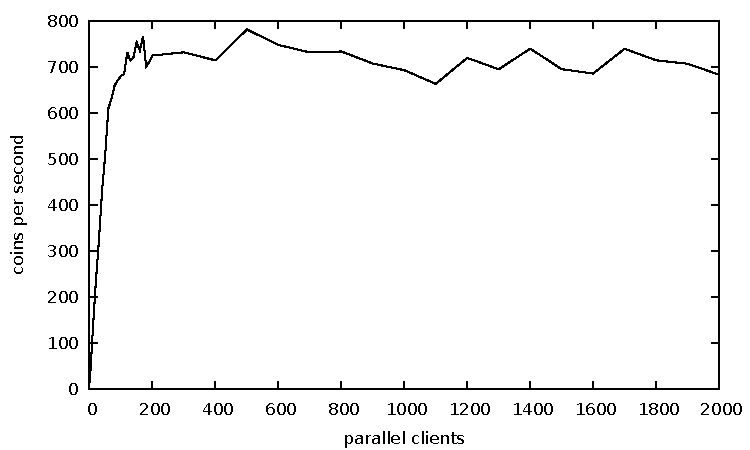
\includegraphics[width=\textwidth]{plots/speed.pdf}
  \caption[Coin throughput.]{Coin throughput in relation to number of parallel clients, with $1000$ coins per client per experiment run.}
  \label{fig:benchmark-throughput}
\end{figure}

\begin{figure}
  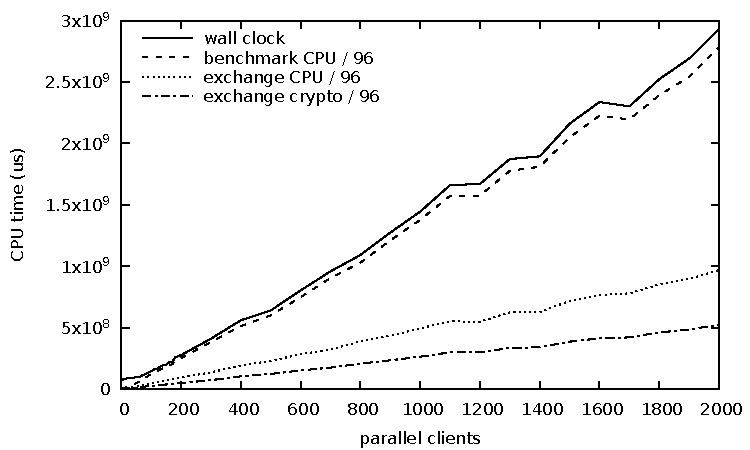
\includegraphics[width=\textwidth]{plots/cpu.pdf}
  \caption[Comparison of components' CPU usage for the benchmark.]{Comparison of real time, the CPU time for the exchange and the whole benchmark.}
  \label{fig:benchmark-cpu}
\end{figure}

\subsection{Latency}
We connected \texttt{firefly} and \texttt{gv} directly with a patch cable, and
introduced artificial network latency by configuring the Linux packet scheduler
with the \texttt{tc} tool.  The goal of this experiment was to observe the
network latency characteristics of the implementation.  Note that we do not consider
the overhead of TLS in our experiments, as we assume that TLS traffic is
already terminated before it reaches the exchange service, and exchanges can be
operated securely even without TLS.

The comparison between no additional delay and a \SI{100}{\milli\second} delay
is shown in Table~\ref{table:latency}.  TCP Fast Open~\cite{rfc7413} was
enabled on both \texttt{gv} and \texttt{firefly}.  Since for all operations
except \texttt{/refresh/reveal}, both request and response fit into one TCP
segment, these operations complete within one round-trip time.  This explains the
additional delay of $\approx \SI{200}{\milli\second}$ when the artificial delay
is introduced.  Without TCP Fast Open, we would observe an extra round trip for
the SYN and SYN/ACK packages without any payload.  The \texttt{/refresh/reveal}
operation takes an extra roundtrip due to the relatively large size of the
request (as show in Table~\ref{table:api-size}), which exceeds the MTU of 1500
for the link between \texttt{gv} and \texttt{firefly}, and thus does not fit
into the first TCP Fast Open packet.

Figure~\ref{fig:latencies} shows the latency for the exchange's HTTP endpoints
in relation to different network delays.  As expected, the additional delay
grows linearly for a single client.  We note that in larger benchmarks with
multiple parallel clients, the effect of additional delay would likely not just
be linear, due to timeouts raised by clients.

\newcommand{\specialcell}[2][c]{%
  \begin{tabular}[#1]{@{}c@{}}#2\end{tabular}}

\begin{table}
  \centering
  \begin{tabular}{lSSSS}
  \toprule
    Endpoint &
    {\specialcell[c]{Base latency\\(\si{\milli\second})}} &
    {\specialcell[c]{Latency with\\\SI{100}{\milli\second} delay\\(\si{\milli\second})}} \\
  \midrule
    \texttt{/keys}                &  1.14   &    201.25   \\ 
    \texttt{/reserve/withdraw}    &  22.68  &    222.46   \\ 
    \texttt{/deposit}             &  22.36  &   223.22    \\
    \texttt{/refresh/melt}        &  20.71  &    223.9    \\ 
    \texttt{/refresh/reveal}      &  63.64  &   466.30    \\
  \bottomrule
  \end{tabular}
  \caption{Effects of \SI{100}{\milli\second} symmetric network delay on total latency.}
  \label{table:latency}
\end{table}

\begin{table}
  \centering
  \begin{tabular}{lSSSS}
  \toprule
    Endpoint &
    {\specialcell[c]{Request size\\2048-bit RSA\\(\si{\kilo\byte})}} &
    {\specialcell[c]{Response size\\2048-bit RSA\\(\si{\kilo\byte})}} &
    {\specialcell[c]{Request size\\1024-bit RSA\\(\si{\kilo\byte})}} &
    {\specialcell[c]{Response size\\1024-bit RSA\\(\si{\kilo\byte})}} \\
  \midrule
    \texttt{/keys}                 & 0.14  & 3.75 & 0.14 & 3.43  \\ 
    \texttt{/reserve/withdraw}     & 0.73   & 0.71 & 0.60 & 0.49 \\ 
    \texttt{/deposit}              & 1.40   & 0.34 & 1.14 & 0.24  \\
    \texttt{/refresh/melt}         & 1.06   & 0.35 & 0.85 & 0.35  \\ 
    \texttt{/refresh/reveal}       & 1.67   & 2.11 & 1.16 & 1.23 \\
  \bottomrule
  \end{tabular}
  \caption[Request and response sizes for the exchange's API.]{Request and response sizes for the exchange's API.
  In addition to the sizes for 2048-bit RSA keys (used throughout the benchmark), the sizes for 1024-bit RSA keys are also provided.}
  \label{table:api-size}
\end{table}

\begin{figure}
  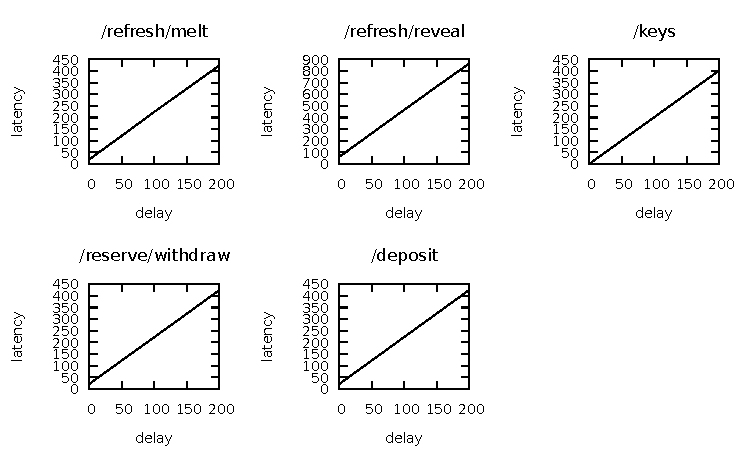
\includegraphics[width=\textwidth]{plots/latencies.pdf}
  \caption[Effect of artificial network delay on exchange's latency.]{Effect of artificial network delay on exchange's latency.}
  \label{fig:latencies}
\end{figure}

% Missing benchmarks:
% overall Taler tx/s
% db io+tx/s
% If I have time:
% traffic/storage depending on key size?


\section{Current Limitations and Future Improvements}\label{sec:implementation-improvements}
Currently the auditor does not support taking samples of deposit confirmations that
merchants receive.  The API and user interface to receive and process proofs
of misbehavior of the exchange/merchant generated by the wallet is not implemented yet.

As a real-world deployment of electronic cash has rather high requirements for
the operational security, the usage of hardware security modules for generation
of signatures should be considered.  Currently, a single process has access to
all key material.  For a lower-cost improvement that decreases the performance
of the system, a threshold signature scheme could be used.

The current implementation is focused on web payments.  To use GNU Taler for
payments in brick-and-mortar stores, hardware wallets and smartphone apps for
devices with near-field-communication (NFC) must be developed.  In some
scenarios, either the customer or the merchant might not have an Internet
connection, and this must be considered in the protocol design.  In typical
western brick-and-mortar stores, it is currently more likely that the merchant
has Internet connectivity, and thus the protocol must allow operations of the
wallet (such as refreshing) to be securely routed over the merchant's
connection.  In other scenarios, typically in developing countries, the
merchant (for example, a street vendor) might not have Internet connection.  If
the vendor has a smartphone, the connection to the merchant can be routed
through the customer.  In other cases, street vendors only have a ``dumb
phone'' that can receive text messages, and the payment goes through a provider
trusted by the merchant that sends text messages as confirmation for payments.
All these possibilities must be considered both from the perspective of the procotol and APIs
as well as the user experience.

% FIXME: explain that exchange does threading

Our experiments were only done with single exchange process and a single
database on the same machine.  There are various ways to horizontally scale the
exchange:
\begin{itemize}
  \item Multiple exchange processes can be run on multiple machines and access
    the database that runs a separate machine.  Requests are directed to the
    machines running the exchange process via a load balancer.  In this
    scenario, the throughput of the database is likely to be the bottleneck.
  \item To avoid having the database as a bottleneck, the contents can be
    partitioned into shards.  For this technique to be effective, data in the
    shards should not have any dependencies in other shards. A natural way to
    do sharding for the Taler exchange is to give each shard the sole
    responsibility for a subset of all available denominations.
  \item If the transaction volume on one denomination is too high to handle for
    a single shard, transactions can be further partitioned based on the coin's
    public key.  Each would maintain the database of spent/refreshed coins for
    a subset of all possible coin public keys.  This approach has been
    suggested for a centrally-banked cryprocurrency by Danezis and Meiklejohn
    \cite{danezis2016rscoin}.
\end{itemize}

% paranoid wallet (permissions!)

% FIXME: I want to mention PADs for auditing/transparency somewhere, just
% because they're cool


% FIXME:  coin locking not implemented!

\chapter{Future Work}\label{chapter:future-work}
We now discuss future work that builds upon the results presented so far.


\subsection*{Standard Model}
Our current instantiation of the Taler protocol relies heavily on hash
functions.  Since the result by Canetti and others \cite{canetti2004random}
about the theoretical impossibility of securely instantiating protocols that
rely on the random oracle assumption for their security, a vast amount of
literature has been devoted to find instantiations of interesting protocols in
the standard model \cite{koblitz2015random}.  The Taler protocol syntax could
likely be also instantiated securely in the standard model, based existing on
blind signature schemes in the standard model.  The trade-off however is that
while removing the random oracle assumption, typically other less well known
assumptions must be made.

\subsection*{Post-Quantum security}
The possibility of post-quantum computers breaking the security of established
cryptographic primitives has lately received a lot of attention from
cryptographers.  While currently most schemes with post-quantum security are impractical,
it might be worthwhile to further investigate their application to e-cash, based
on existing work such as \cite{zhang2018new}.

\subsection*{Applications to network incentives}
Some peer-to-peer networking protocols (such as onion routing
\cite{dingledine2004tor}) do not have inherent incentives and rely on
volunteers to provide infrastructure.  In future work, we want to look at
adding incentives in the form of Taler payments to a peer-to-peer networking
platform such as GNUnet.

\subsection*{Smart(er) Contracts and Auctions}
Contract terms in Taler are relatively limited.  There are some interesting
secure multiparty computations, such as privacy-preserving auctions
\cite{brandt2006obtain} that could be offered by exchanges as a fixed smart
contract.  This would allow a full privacy-preserving auction platform, as
current auction protocols only output the winner of a privacy-preserving
auction but do not address the required anonymous payments.


\subsection*{Backup and Sync}\label{sec:future-work-backup-sync}
Synchronization of wallets between multiple devices is a useful feature, but a
na\"ive implementation endangers privacy.  A carefully designed protocol for
backup and synchronization must make sure that the hosting service for the
wallet's data cannot collaborate with the exchange and merchants to deanonymize
users or transactions.  Thus when spending coins for a payment, devices should
not have to synchronously talk to their backup/sync provider.  This creates the
challenge of allocating the total available balance to individual devices in a
way that fits the customer's spending pattern, and only require synchronous
communication at fixed intervals or when really necessary to re-allocate coins.

Another possible approach might be to use Private Information Retrieval (PIR)
\cite{goldberg2007improving} to access backup and synchronization information.


\subsection*{Machine-Verified Proofs}
We currently model only a subset of the GNU Taler protocol formally, and proofs
are handwritten and verified by humans.  A tool such as CryptoVerif
\cite{blanchet2007cryptoverif} can allow a higher coverage and computer-checked
proofs, and would allow protocol changes to be validated in shorter time.

\subsection*{Coin Restrictions / ``Taler for Children''}
By designating certain denominations for different purposes, GNU Taler could be
used to implement a very simple form of anonymous credentials
\cite{paquin2011u,camenisch2004signature}, which then could be used to
implement a Taler wallet specifically aimed at children, in order to teach them
responsible and autonomous spending behavior, while granting them privacy and
at the same time preventing them from making age-inappropriate purchases
online, as the discretion of parents.

%\subsection*{gnunet-blockchain / deployment of the full stack payment system}
%=> no, talk more about integration with real banks, KYC
%
%\subsection*{P2P payments}
%
%\subsection*{NFC Wallet}
%
%\subsection*{large, scaleable deployment}
%I.e. sharding, db replication, load balancer(s)
%
%\subsection*{Hardware security module for exchange}
%
%\subsection*{Bitcoin/Blockchain integration}
%
%\subsection*{UX study and improvements}
%(including tracking/planning of spending)
%
%\subsection*{News Distribution}

\chapter{Conclusion}\label{chapter:conclusion}

% sources and inspirations
% https://www.bis.org/publ/arpdf/ar2018e5.pdf
% https://www.bis.org/publ/qtrpdf/r_qt1709f.pdf
% http://andolfatto.blogspot.com/2015/02/fedcoin-on-desirability-of-government.html

% mention eKrona/Riksbank

% bessere ueberleitung
% effizienz!
% freie software / commons
% scalability of blockchains
% expand on some ideas such as naiveity of blockchains
% 3 areas for currencies


% einleitung: we introduced two systems that solve/address core problems for
% banking (consensus, transactions, ...) "geld ist kein selbstzweck"
% reason for having money is: ...

% central banks are the only tool that we know that works

% geld ist politisch, macht, verantwortung, gesellschaften aufbauen oder ruinieren
% apolitical solution impossible

This book presented GNU Taler, an efficient protocol for
value-based electronic payment systems with focus on security and
privacy.  While we believe our approach to be socially and economically beneficial, a
technological impact analysis is in order prior to adopting new
systems that have broad economic and socio-political implications.

Currencies serve three key functions in society:~\cite{mankiw2010macroeconomics}
\begin{enumerate}
\item As a unit for measurement of value,
\item a medium of exchange, and
\item a store of value.
\end{enumerate}
How do the various methods measure up to these requirements?

\section{Cryptocurrencies vs. Central-Bank-Issued Currencies}

\begin{figure}
\centering
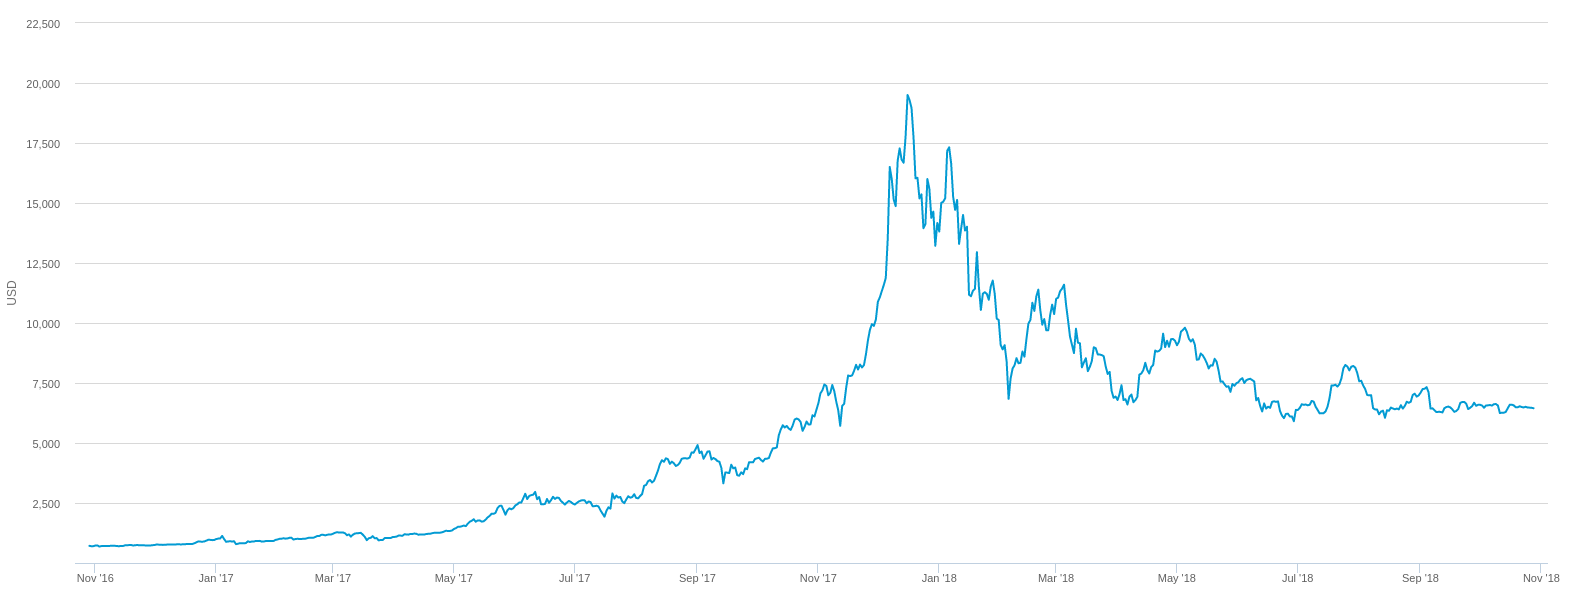
\includegraphics[width=\textwidth]{diagrams/bitcoin-market-price.png}
  \caption[Historical market price of Bitcoin.]{Historical market price (in
  USD) of Bitcoin across major exchanges (Source:~\url{https://blockchain.com}).}
\label{fig:volatility}
\end{figure}

Cryptocurrencies generally fail to achieve the required stability to serve as a
reasonable unit of measurement (Figure~\ref{fig:volatility}).  The volatility
of cyptocurrencies is caused by a combination of a lack of institutions that
could intervene to dampen fluctuations and a comparatively limited liquidity
in the respective
markets.  The latter is exacerbated by the limited ability of decentralized
cryptocurrencies to handle large transaction volumes, despite their extreme
levels of resource consumption.  As a result, the utility of decentralized
cryptocurrencies is limited to highly speculative investments and to the
facilitation of criminal transactions.

With respect to privacy, completely decentralized cryptocurrencies
provide either too much or too little anonymity.  Transparent
cryptocurrencies create the spectre of discriminatory pricing, while
especially for privacy-enhanced cryptocurrencies the lack of
regulation creates an attractive environment for fraud and criminal
activity from tax evasion to financing of terrorism.

These problems are easily addressed by combining the register (or
ledger) with a central bank providing a regulatory framework and
monetary policy, including anti-money-laundering and
know-your-customer enforcement.  

\section{Electronic Payments}

Day-to-day payments using registers are expensive and inconvenient.
Using a register requires users to {\em identify} themselves to {\em
  authorize} transactions, and the use of register-based banking
systems tends to be more expensive than the direct exchange of
physical cash.  However, with the ongoing digitalization of daily life
where a significant number of transactions is realized over networks,
some form of electronic payments remain inevitable.

The current alternative to (centrally banked) electronic cash are a
payment systems under full control of oligopoly companies such as
Google, Apple, Facebook or Visa.  The resulting oligopolies are
anti-competitive. In addition to excessive fees, they sometimes even
refuse to process payments with certain types of legal businesses,
which then are often ruined due to lack of alternatives.  Combining
payment services with companies where the core business model is
advertising is also particularly damaging for privacy.  Finally, the
sheer size of these companies creates systemic risks, just as their
global scale creates challenges for regulation.

As GNU Taler is free software, even without backing by a central bank,
Taler would not suffer from these drawbacks arising from the use of
proprietary technology.

Furthermore, Taler-style electronic cash comes
with some unique benefits:
\begin{itemize}
  \item improved income transparency compared to cash and traditional
    Chaum-style e-cash,
  \item anonymity for payers,
  \item avoidance of enticement towards consumer debt --- especially
    compared to credit cards, and
  \item support of new business models and Internet security
    mechanisms which require (anonymous) micro-transactions.
\end{itemize}

Central banks are carefully considering what might be the right
technology to implement an electronic version of their centrally
banked currency, and with Taler we hope to address most of their concerns.
Nevertheless, all electronic payment systems, including Taler even
when backed by central-bank-issued currencies, come with their own
inherent set of risks:~\cite{riksbank2017riksbank}

\begin{itemize}
  \item increased risk of a bank run: in a banking crisis,
    as it is easier to withdraw large amounts of digital
    cash quickly --- even from remote locations;
  \item increased volatility due to foreign holdings that would
    not be as easily possible with physical cash;
  \item increased risk of theft and disruption: while physical
    cash can also be stolen (and likely with much less effort), it is
    difficult to transport in volume~\cite{force2015money}, the
    risk is increased with computers because attacks scale \cite{hammer2018billion}, and
    generally many small incidents are socially preferable over a
    tiny number of very large-scale incidents; and
  \item unavailability in crisis situations without electricity and Internet
    connectivity.
\end{itemize}


We believe that in the case of Taler, some of the risks mentioned
above can be mitigated:
\begin{itemize}
 \item Volatility due to foreign holdings and the resulting increased
   risk of bank runs can be reduced by putting limits on the amount of
   electronic coins that customers can withdraw.  Limiting the
   validity periods of coins is another method that can help
   disincentivize the use of Taler as a value store.
 \item The use of open standards and reference implementations enables
   white-hat security research around GNU Taler, which together with
   good operational security procedures and the possibility of
   competing providers should reduce the risks from attacks.
 \item GNU Taler can co-exist with physical cash, and might even
   help revive the use of cash if it succeeds in reducing credit
   card use online thereby eliminating a key reason for people to
   have credit cards.
\end{itemize}

Unlike cryptocurrencies, Taler does not prescribe a solution for monetary
policy or just taxation, as we believe these issues need to be subject to
continuous political debate and cannot be ``solved'' by simplistic algorithms.
What we offer to society is an open and free (as in free speech) system with
mechanisms to audit merchants' income, instead of proprietary systems
controlled by a few oligopoly companies.



\printbibliography[heading=bibintoc]

\end{document}
